% This must be in the first 5 lines to tell arXiv to use pdfLaTeX, which is strongly recommended.
\pdfoutput=1
% In particular, the hyperref package requires pdfLaTeX in order to break URLs across lines.

\documentclass[11pt]{article}

% Change "review" to "final" to generate the final (sometimes called camera-ready) version.
% Change to "preprint" to generate a non-anonymous version with page numbers.
\usepackage[final]{acl}

% Standard package includes
\usepackage{times}
\usepackage{latexsym}
\usepackage{url}

% For proper rendering and hyphenation of words containing Latin characters (including in bib files)
\usepackage[T1]{fontenc}
% For Vietnamese characters
% \usepackage[T5]{fontenc}
% See https://www.latex-project.org/help/documentation/encguide.pdf for other character sets

% This assumes your files are encoded as UTF8
\usepackage[utf8]{inputenc}

% This is not strictly necessary, and may be commented out,
% but it will improve the layout of the manuscript,
% and will typically save some space.
\usepackage{microtype}

% This is also not strictly necessary, and may be commented out.
% However, it will improve the aesthetics of text in
% the typewriter font.
\usepackage{inconsolata}

%Including images in your LaTeX document requires adding
%additional package(s)
\usepackage{graphicx}

% Standard package includes
\usepackage{times}
\usepackage{booktabs}
\usepackage{latexsym}
\usepackage{algorithm}
\usepackage{multirow, multicol}

%\usepackage{algorithmic}
\usepackage{bbm}
\usepackage{algpseudocode}
\usepackage{amsmath}
\usepackage{soul}
\usepackage{pifont}
\usepackage{paralist}
\usepackage[most]{tcolorbox}
\definecolor{green1}{RGB}{215, 255, 215}  % Medium light green
\definecolor{green2}{RGB}{138, 209, 138}  % Medium green

\newcommand{\sa}[1]{\textcolor{red}{\{#1 -- SA\}}}
\newcommand{\mo}[1]{\textcolor{red}{#1 -- MC}}

\newcommand{\skp}[1]{\textcolor{blue}{#1 -- SKP}}
\newcommand{\sv}[1]{\textcolor{blue}{#1 -- SV}}
\newcommand{\dd}[1]{\textcolor{blue}{#1 -- DD}}


\algnewcommand\algorithmicinput{\textbf{Input:}}
\algnewcommand\INPUT{\item[\algorithmicinput]}

\algnewcommand\algorithmicrepresentation{\textbf{Representation:}}
\algnewcommand\REPRESENTATION{\item[\algorithmicrepresentation]}

\algnewcommand\algorithmicoutput{\textbf{Output:}}
\algnewcommand\OUTPUT{\item[\algorithmicoutput]}


\usepackage{tikz}
\newcommand*\circled[1]{\tikz[baseline=(char.base)]{
        \node[shape=circle,draw,inner sep=1pt] (char) {#1};}}


\usepackage{graphicx}
\usepackage{amssymb}
\usepackage{inconsolata}

% If the title and author information does not fit in the area allocated, uncomment the following
%
%\setlength\titlebox{<dim>}
%
% and set <dim> to something 5cm or larger.

\title{SMAB: MAB based word Sensitivity Estimation Framework and its Applications in Adversarial Text Generation}

% Author information can be set in various styles:
% For several authors from the same institution:
% \author{Author 1 \and ... \and Author n \\
%         Address line \\ ... \\ Address line}
% if the names do not fit well on one line use
%         Author 1 \\ {\bf Author 2} \\ ... \\ {\bf Author n} \\
% For authors from different institutions:
% \author{Author 1 \\ Address line \\  ... \\ Address line
%         \And  ... \And
%         Author n \\ Address line \\ ... \\ Address line}
% To start a separate ``row'' of authors use \AND, as in
% \author{Author 1 \\ Address line \\  ... \\ Address line
%         \AND
%         Author 2 \\ Address line \\ ... \\ Address line \And
%         Author 3 \\ Address line \\ ... \\ Address line}

% \author{First Author \\
%   Affiliation / Address line 1 \\
%   Affiliation / Address line 2 \\
%   Affiliation / Address line 3 \\
%   \texttt{email@domain} \\\And
%   Second Author \\
%   Affiliation / Address line 1 \\
%   Affiliation / Address line 2 \\
%   Affiliation / Address line 3 \\
%   \texttt{email@domain} \\}

\author{
\textbf{Saurabh Kumar Pandey\textsuperscript{1*}},
  \textbf{Sachin Vashistha\textsuperscript{2*}},
  \textbf{Debrup Das\textsuperscript{3}},
\\
  \textbf{Somak Aditya\textsuperscript{2}},
  \textbf{Monojit Choudhury\textsuperscript{1}}
  \\ 
  \texttt{saurabh2000.iitkgp@gmail.com, sachinvashistha6916@gmail.com,}
\\
  \texttt{saditya@cse.iitkgp.ac.in, monojit.choudhury@mbzuai.ac.ae}
   \\
  \textsuperscript{1}MBZUAI, 
  \\
  \textsuperscript{2}Indian Institute of Technology, Kharagpur
  \\
  \textsuperscript{3}University of Massachusetts Amherst 
%  \textsuperscript{5}Affiliation 5
%\\
}

%\author{
%  \textbf{First Author\textsuperscript{1}},
%  \textbf{Second Author\textsuperscript{1,2}},
%  \textbf{Third T. Author\textsuperscript{1}},
%  \textbf{Fourth Author\textsuperscript{1}},
%\\
%  \textbf{Fifth Author\textsuperscript{1,2}},
%  \textbf{Sixth Author\textsuperscript{1}},
%  \textbf{Seventh Author\textsuperscript{1}},
%  \textbf{Eighth Author \textsuperscript{1,2,3,4}},
%\\
%  \textbf{Ninth Author\textsuperscript{1}},
%  \textbf{Tenth Author\textsuperscript{1}},
%  \textbf{Eleventh E. Author\textsuperscript{1,2,3,4,5}},
%  \textbf{Twelfth Author\textsuperscript{1}},
%\\
%  \textbf{Thirteenth Author\textsuperscript{3}},
%  \textbf{Fourteenth F. Author\textsuperscript{2,4}},
%  \textbf{Fifteenth Author\textsuperscript{1}},
%  \textbf{Sixteenth Author\textsuperscript{1}},
%\\
%  \textbf{Seventeenth S. Author\textsuperscript{4,5}},
%  \textbf{Eighteenth Author\textsuperscript{3,4}},
%  \textbf{Nineteenth N. Author\textsuperscript{2,5}},
%  \textbf{Twentieth Author\textsuperscript{1}}
%\\
%\\
%  \textsuperscript{1}Affiliation 1,
%  \textsuperscript{2}Affiliation 2,
%  \textsuperscript{3}Affiliation 3,
%  \textsuperscript{4}Affiliation 4,
%  \textsuperscript{5}Affiliation 5
%\\
%  \small{
%    \textbf{Correspondence:} \href{mailto:email@domain}{email@domain}
%  }
%}

\begin{document}
\maketitle

\setlength{\abovedisplayskip}{1pt}
\setlength{\belowdisplayskip}{1pt}

\begin{abstract}
\begin{abstract}  
Test time scaling is currently one of the most active research areas that shows promise after training time scaling has reached its limits.
Deep-thinking (DT) models are a class of recurrent models that can perform easy-to-hard generalization by assigning more compute to harder test samples.
However, due to their inability to determine the complexity of a test sample, DT models have to use a large amount of computation for both easy and hard test samples.
Excessive test time computation is wasteful and can cause the ``overthinking'' problem where more test time computation leads to worse results.
In this paper, we introduce a test time training method for determining the optimal amount of computation needed for each sample during test time.
We also propose Conv-LiGRU, a novel recurrent architecture for efficient and robust visual reasoning. 
Extensive experiments demonstrate that Conv-LiGRU is more stable than DT, effectively mitigates the ``overthinking'' phenomenon, and achieves superior accuracy.
\end{abstract}  
\let\thefootnote\relax\footnotetext[1]{* indicates equal contribution, Order chosen at random}
\end{abstract}

% \iftaclpubformat

\section{Introduction}
\section{Introduction}
\label{sec:introduction}
The business processes of organizations are experiencing ever-increasing complexity due to the large amount of data, high number of users, and high-tech devices involved \cite{martin2021pmopportunitieschallenges, beerepoot2023biggestbpmproblems}. This complexity may cause business processes to deviate from normal control flow due to unforeseen and disruptive anomalies \cite{adams2023proceddsriftdetection}. These control-flow anomalies manifest as unknown, skipped, and wrongly-ordered activities in the traces of event logs monitored from the execution of business processes \cite{ko2023adsystematicreview}. For the sake of clarity, let us consider an illustrative example of such anomalies. Figure \ref{FP_ANOMALIES} shows a so-called event log footprint, which captures the control flow relations of four activities of a hypothetical event log. In particular, this footprint captures the control-flow relations between activities \texttt{a}, \texttt{b}, \texttt{c} and \texttt{d}. These are the causal ($\rightarrow$) relation, concurrent ($\parallel$) relation, and other ($\#$) relations such as exclusivity or non-local dependency \cite{aalst2022pmhandbook}. In addition, on the right are six traces, of which five exhibit skipped, wrongly-ordered and unknown control-flow anomalies. For example, $\langle$\texttt{a b d}$\rangle$ has a skipped activity, which is \texttt{c}. Because of this skipped activity, the control-flow relation \texttt{b}$\,\#\,$\texttt{d} is violated, since \texttt{d} directly follows \texttt{b} in the anomalous trace.
\begin{figure}[!t]
\centering
\includegraphics[width=0.9\columnwidth]{images/FP_ANOMALIES.png}
\caption{An example event log footprint with six traces, of which five exhibit control-flow anomalies.}
\label{FP_ANOMALIES}
\end{figure}

\subsection{Control-flow anomaly detection}
Control-flow anomaly detection techniques aim to characterize the normal control flow from event logs and verify whether these deviations occur in new event logs \cite{ko2023adsystematicreview}. To develop control-flow anomaly detection techniques, \revision{process mining} has seen widespread adoption owing to process discovery and \revision{conformance checking}. On the one hand, process discovery is a set of algorithms that encode control-flow relations as a set of model elements and constraints according to a given modeling formalism \cite{aalst2022pmhandbook}; hereafter, we refer to the Petri net, a widespread modeling formalism. On the other hand, \revision{conformance checking} is an explainable set of algorithms that allows linking any deviations with the reference Petri net and providing the fitness measure, namely a measure of how much the Petri net fits the new event log \cite{aalst2022pmhandbook}. Many control-flow anomaly detection techniques based on \revision{conformance checking} (hereafter, \revision{conformance checking}-based techniques) use the fitness measure to determine whether an event log is anomalous \cite{bezerra2009pmad, bezerra2013adlogspais, myers2018icsadpm, pecchia2020applicationfailuresanalysispm}. 

The scientific literature also includes many \revision{conformance checking}-independent techniques for control-flow anomaly detection that combine specific types of trace encodings with machine/deep learning \cite{ko2023adsystematicreview, tavares2023pmtraceencoding}. Whereas these techniques are very effective, their explainability is challenging due to both the type of trace encoding employed and the machine/deep learning model used \cite{rawal2022trustworthyaiadvances,li2023explainablead}. Hence, in the following, we focus on the shortcomings of \revision{conformance checking}-based techniques to investigate whether it is possible to support the development of competitive control-flow anomaly detection techniques while maintaining the explainable nature of \revision{conformance checking}.
\begin{figure}[!t]
\centering
\includegraphics[width=\columnwidth]{images/HIGH_LEVEL_VIEW.png}
\caption{A high-level view of the proposed framework for combining \revision{process mining}-based feature extraction with dimensionality reduction for control-flow anomaly detection.}
\label{HIGH_LEVEL_VIEW}
\end{figure}

\subsection{Shortcomings of \revision{conformance checking}-based techniques}
Unfortunately, the detection effectiveness of \revision{conformance checking}-based techniques is affected by noisy data and low-quality Petri nets, which may be due to human errors in the modeling process or representational bias of process discovery algorithms \cite{bezerra2013adlogspais, pecchia2020applicationfailuresanalysispm, aalst2016pm}. Specifically, on the one hand, noisy data may introduce infrequent and deceptive control-flow relations that may result in inconsistent fitness measures, whereas, on the other hand, checking event logs against a low-quality Petri net could lead to an unreliable distribution of fitness measures. Nonetheless, such Petri nets can still be used as references to obtain insightful information for \revision{process mining}-based feature extraction, supporting the development of competitive and explainable \revision{conformance checking}-based techniques for control-flow anomaly detection despite the problems above. For example, a few works outline that token-based \revision{conformance checking} can be used for \revision{process mining}-based feature extraction to build tabular data and develop effective \revision{conformance checking}-based techniques for control-flow anomaly detection \cite{singh2022lapmsh, debenedictis2023dtadiiot}. However, to the best of our knowledge, the scientific literature lacks a structured proposal for \revision{process mining}-based feature extraction using the state-of-the-art \revision{conformance checking} variant, namely alignment-based \revision{conformance checking}.

\subsection{Contributions}
We propose a novel \revision{process mining}-based feature extraction approach with alignment-based \revision{conformance checking}. This variant aligns the deviating control flow with a reference Petri net; the resulting alignment can be inspected to extract additional statistics such as the number of times a given activity caused mismatches \cite{aalst2022pmhandbook}. We integrate this approach into a flexible and explainable framework for developing techniques for control-flow anomaly detection. The framework combines \revision{process mining}-based feature extraction and dimensionality reduction to handle high-dimensional feature sets, achieve detection effectiveness, and support explainability. Notably, in addition to our proposed \revision{process mining}-based feature extraction approach, the framework allows employing other approaches, enabling a fair comparison of multiple \revision{conformance checking}-based and \revision{conformance checking}-independent techniques for control-flow anomaly detection. Figure \ref{HIGH_LEVEL_VIEW} shows a high-level view of the framework. Business processes are monitored, and event logs obtained from the database of information systems. Subsequently, \revision{process mining}-based feature extraction is applied to these event logs and tabular data input to dimensionality reduction to identify control-flow anomalies. We apply several \revision{conformance checking}-based and \revision{conformance checking}-independent framework techniques to publicly available datasets, simulated data of a case study from railways, and real-world data of a case study from healthcare. We show that the framework techniques implementing our approach outperform the baseline \revision{conformance checking}-based techniques while maintaining the explainable nature of \revision{conformance checking}.

In summary, the contributions of this paper are as follows.
\begin{itemize}
    \item{
        A novel \revision{process mining}-based feature extraction approach to support the development of competitive and explainable \revision{conformance checking}-based techniques for control-flow anomaly detection.
    }
    \item{
        A flexible and explainable framework for developing techniques for control-flow anomaly detection using \revision{process mining}-based feature extraction and dimensionality reduction.
    }
    \item{
        Application to synthetic and real-world datasets of several \revision{conformance checking}-based and \revision{conformance checking}-independent framework techniques, evaluating their detection effectiveness and explainability.
    }
\end{itemize}

The rest of the paper is organized as follows.
\begin{itemize}
    \item Section \ref{sec:related_work} reviews the existing techniques for control-flow anomaly detection, categorizing them into \revision{conformance checking}-based and \revision{conformance checking}-independent techniques.
    \item Section \ref{sec:abccfe} provides the preliminaries of \revision{process mining} to establish the notation used throughout the paper, and delves into the details of the proposed \revision{process mining}-based feature extraction approach with alignment-based \revision{conformance checking}.
    \item Section \ref{sec:framework} describes the framework for developing \revision{conformance checking}-based and \revision{conformance checking}-independent techniques for control-flow anomaly detection that combine \revision{process mining}-based feature extraction and dimensionality reduction.
    \item Section \ref{sec:evaluation} presents the experiments conducted with multiple framework and baseline techniques using data from publicly available datasets and case studies.
    \item Section \ref{sec:conclusions} draws the conclusions and presents future work.
\end{itemize}

\section{Methodology}
\section{Research Methodology}~\label{sec:Methodology}

In this section, we discuss the process of conducting our systematic review, e.g., our search strategy for data extraction of relevant studies, based on the guidelines of Kitchenham et al.~\cite{kitchenham2022segress} to conduct SLRs and Petersen et al.~\cite{PETERSEN20151} to conduct systematic mapping studies (SMSs) in Software Engineering. In this systematic review, we divide our work into a four-stage procedure, including planning, conducting, building a taxonomy, and reporting the review, illustrated in Fig.~\ref{fig:search}. The four stages are as follows: (1) the \emph{planning} stage involved identifying research questions (RQs) and specifying the detailed research plan for the study; (2) the \emph{conducting} stage involved analyzing and synthesizing the existing primary studies to answer the research questions; (3) the \emph{taxonomy} stage was introduced to optimize the data extraction results and consolidate a taxonomy schema for REDAST methodology; (4) the \emph{reporting} stage involved the reviewing, concluding and reporting the final result of our study.

\begin{figure}[!t]
    \centering
    \includegraphics[width=1\linewidth]{fig/methodology/searching-process.drawio.pdf}
    \caption{Systematic Literature Review Process}
    \label{fig:search}
\end{figure}

\subsection{Research Questions}
In this study, we developed five research questions (RQs) to identify the input and output, analyze technologies, evaluate metrics, identify challenges, and identify potential opportunities. 

\textbf{RQ1. What are the input configurations, formats, and notations used in the requirements in requirements-driven
automated software testing?} In requirements-driven testing, the input is some form of requirements specification -- which can vary significantly. RQ1 maps the input for REDAST and reports on the comparison among different formats for requirements specification.

\textbf{RQ2. What are the frameworks, tools, processing methods, and transformation techniques used in requirements-driven automated software testing studies?} RQ2 explores the technical solutions from requirements to generated artifacts, e.g., rule-based transformation applying natural language processing (NLP) pipelines and deep learning (DL) techniques, where we additionally discuss the potential intermediate representation and additional input for the transformation process.

\textbf{RQ3. What are the test formats and coverage criteria used in the requirements-driven automated software
testing process?} RQ3 focuses on identifying the formulation of generated artifacts (i.e., the final output). We map the adopted test formats and analyze their characteristics in the REDAST process.

\textbf{RQ4. How do existing studies evaluate the generated test artifacts in the requirements-driven automated software testing process?} RQ4 identifies the evaluation datasets, metrics, and case study methodologies in the selected papers. This aims to understand how researchers assess the effectiveness, accuracy, and practical applicability of the generated test artifacts.

\textbf{RQ5. What are the limitations and challenges of existing requirements-driven automated software testing methods in the current era?} RQ5 addresses the limitations and challenges of existing studies while exploring future directions in the current era of technology development. %It particularly highlights the potential benefits of advanced LLMs and examines their capacity to meet the high expectations placed on these cutting-edge language modeling technologies. %\textcolor{blue}{CA: Do we really need to focus on LLMs? TBD.} \textcolor{orange}{FW: About LLMs, I removed the direct emphase in RQ5 but kept the discussion in RQ5 and the solution section. I think that would be more appropriate.}

\subsection{Searching Strategy}

The overview of the search process is exhibited in Fig. \ref{fig:papers}, which includes all the details of our search steps.
\begin{table}[!ht]
\caption{List of Search Terms}
\label{table:search_term}
\begin{tabularx}{\textwidth}{lX}
\hline
\textbf{Terms Group} & \textbf{Terms} \\ \hline
Test Group & test* \\
Requirement Group & requirement* OR use case* OR user stor* OR specification* \\
Software Group & software* OR system* \\
Method Group & generat* OR deriv* OR map* OR creat* OR extract* OR design* OR priorit* OR construct* OR transform* \\ \hline
\end{tabularx}
\end{table}

\begin{figure}
    \centering
    \includegraphics[width=1\linewidth]{fig/methodology/search-papers.drawio.pdf}
    \caption{Study Search Process}
    \label{fig:papers}
\end{figure}

\subsubsection{Search String Formulation}
Our research questions (RQs) guided the identification of the main search terms. We designed our search string with generic keywords to avoid missing out on any related papers, where four groups of search terms are included, namely ``test group'', ``requirement group'', ``software group'', and ``method group''. In order to capture all the expressions of the search terms, we use wildcards to match the appendix of the word, e.g., ``test*'' can capture ``testing'', ``tests'' and so on. The search terms are listed in Table~\ref{table:search_term}, decided after iterative discussion and refinement among all the authors. As a result, we finally formed the search string as follows:


\hangindent=1.5em
 \textbf{ON ABSTRACT} ((``test*'') \textbf{AND} (``requirement*'' \textbf{OR} ``use case*'' \textbf{OR} ``user stor*'' \textbf{OR} ``specifications'') \textbf{AND} (``software*'' \textbf{OR} ``system*'') \textbf{AND} (``generat*'' \textbf{OR} ``deriv*'' \textbf{OR} ``map*'' \textbf{OR} ``creat*'' \textbf{OR} ``extract*'' \textbf{OR} ``design*'' \textbf{OR} ``priorit*'' \textbf{OR} ``construct*'' \textbf{OR} ``transform*''))

The search process was conducted in September 2024, and therefore, the search results reflect studies available up to that date. We conducted the search process on six online databases: IEEE Xplore, ACM Digital Library, Wiley, Scopus, Web of Science, and Science Direct. However, some databases were incompatible with our default search string in the following situations: (1) unsupported for searching within abstract, such as Scopus, and (2) limited search terms, such as ScienceDirect. Here, for (1) situation, we searched within the title, keyword, and abstract, and for (2) situation, we separately executed the search and removed the duplicate papers in the merging process. 

\subsubsection{Automated Searching and Duplicate Removal}
We used advanced search to execute our search string within our selected databases, following our designed selection criteria in Table \ref{table:selection}. The first search returned 27,333 papers. Specifically for the duplicate removal, we used a Python script to remove (1) overlapped search results among multiple databases and (2) conference or workshop papers, also found with the same title and authors in the other journals. After duplicate removal, we obtained 21,652 papers for further filtering.

\begin{table*}[]
\caption{Selection Criteria}
\label{table:selection}
\begin{tabularx}{\textwidth}{lX}
\hline
\textbf{Criterion ID} & \textbf{Criterion Description} \\ \hline
S01          & Papers written in English. \\
S02-1        & Papers in the subjects of "Computer Science" or "Software Engineering". \\
S02-2        & Papers published on software testing-related issues. \\
S03          & Papers published from 1991 to the present. \\ 
S04          & Papers with accessible full text. \\ \hline
\end{tabularx}
\end{table*}

\begin{table*}[]
\small
\caption{Inclusion and Exclusion Criteria}
\label{table:criteria}
\begin{tabularx}{\textwidth}{lX}
\hline
\textbf{ID}  & \textbf{Description} \\ \hline
\multicolumn{2}{l}{\textbf{Inclusion Criteria}} \\ \hline
I01 & Papers about requirements-driven automated system testing or acceptance testing generation, or studies that generate system-testing-related artifacts. \\
I02 & Peer-reviewed studies that have been used in academia with references from literature. \\ \hline
\multicolumn{2}{l}{\textbf{Exclusion Criteria}} \\ \hline
E01 & Studies that only support automated code generation, but not test-artifact generation. \\
E02 & Studies that do not use requirements-related information as an input. \\
E03 & Papers with fewer than 5 pages (1-4 pages). \\
E04 & Non-primary studies (secondary or tertiary studies). \\
E05 & Vision papers and grey literature (unpublished work), books (chapters), posters, discussions, opinions, keynotes, magazine articles, experience, and comparison papers. \\ \hline
\end{tabularx}
\end{table*}

\subsubsection{Filtering Process}

In this step, we filtered a total of 21,652 papers using the inclusion and exclusion criteria outlined in Table \ref{table:criteria}. This process was primarily carried out by the first and second authors. Our criteria are structured at different levels, facilitating a multi-step filtering process. This approach involves applying various criteria in three distinct phases. We employed a cross-verification method involving (1) the first and second authors and (2) the other authors. Initially, the filtering was conducted separately by the first and second authors. After cross-verifying their results, the results were then reviewed and discussed further by the other authors for final decision-making. We widely adopted this verification strategy within the filtering stages. During the filtering process, we managed our paper list using a BibTeX file and categorized the papers with color-coding through BibTeX management software\footnote{\url{https://bibdesk.sourceforge.io/}}, i.e., “red” for irrelevant papers, “yellow” for potentially relevant papers, and “blue” for relevant papers. This color-coding system facilitated the organization and review of papers according to their relevance.

The screening process is shown below,
\begin{itemize}
    \item \textbf{1st-round Filtering} was based on the title and abstract, using the criteria I01 and E01. At this stage, the number of papers was reduced from 21,652 to 9,071.
    \item \textbf{2nd-round Filtering}. We attempted to include requirements-related papers based on E02 on the title and abstract level, which resulted from 9,071 to 4,071 papers. We excluded all the papers that did not focus on requirements-related information as an input or only mentioned the term ``requirements'' but did not refer to the requirements specification.
    \item \textbf{3rd-round Filtering}. We selectively reviewed the content of papers identified as potentially relevant to requirements-driven automated test generation. This process resulted in 162 papers for further analysis.
\end{itemize}
Note that, especially for third-round filtering, we aimed to include as many relevant papers as possible, even borderline cases, according to our criteria. The results were then discussed iteratively among all the authors to reach a consensus.

\subsubsection{Snowballing}

Snowballing is necessary for identifying papers that may have been missed during the automated search. Following the guidelines by Wohlin~\cite{wohlin2014guidelines}, we conducted both forward and backward snowballing. As a result, we identified 24 additional papers through this process.

\subsubsection{Data Extraction}

Based on the formulated research questions (RQs), we designed 38 data extraction questions\footnote{\url{https://drive.google.com/file/d/1yjy-59Juu9L3WHaOPu-XQo-j-HHGTbx_/view?usp=sharing}} and created a Google Form to collect the required information from the relevant papers. The questions included 30 short-answer questions, six checkbox questions, and two selection questions. The data extraction was organized into five sections: (1) basic information: fundamental details such as title, author, venue, etc.; (2) open information: insights on motivation, limitations, challenges, etc.; (3) requirements: requirements format, notation, and related aspects; (4) methodology: details, including immediate representation and technique support; (5) test-related information: test format(s), coverage, and related elements. Similar to the filtering process, the first and second authors conducted the data extraction and then forwarded the results to the other authors to initiate the review meeting.

\subsubsection{Quality Assessment}

During the data extraction process, we encountered papers with insufficient information. To address this, we conducted a quality assessment in parallel to ensure the relevance of the papers to our objectives. This approach, also adopted in previous secondary studies~\cite{shamsujjoha2021developing, naveed2024model}, involved designing a set of assessment questions based on guidelines by Kitchenham et al.~\cite{kitchenham2022segress}. The quality assessment questions in our study are shown below:
\begin{itemize}
    \item \textbf{QA1}. Does this study clearly state \emph{how} requirements drive automated test generation?
    \item \textbf{QA2}. Does this study clearly state the \emph{aim} of REDAST?
    \item \textbf{QA3}. Does this study enable \emph{automation} in test generation?
    \item \textbf{QA4}. Does this study demonstrate the usability of the method from the perspective of methodology explanation, discussion, case examples, and experiments?
\end{itemize}
QA4 originates from an open perspective in the review process, where we focused on evaluation, discussion, and explanation. Our review also examined the study’s overall structure, including the methodology description, case studies, experiments, and analyses. The detailed results of the quality assessment are provided in the Appendix. Following this assessment, the final data extraction was based on 156 papers.

% \begin{table}[]
% \begin{tabular}{ll}
% \hline
% QA ID & QA Questions                                             \\ \hline
% Q01   & Does this study clearly state its aims?                  \\
% Q02   & Does this study clearly describe its methodology?        \\
% Q03   & Does this study involve automated test generation?       \\
% Q04   & Does this study include a promising evaluation?          \\
% Q05   & Does this study demonstrate the usability of the method? \\ \hline
% \end{tabular}%
% \caption{Questions for Quality Assessment}
% \label{table:qa}
% \end{table}

% automated quality assessment

% \textcolor{blue}{CA: Our search strategy focused on identifying requirements types first. We covered several sources, e.g., ~\cite{Pohl:11,wagner2019status} to identify different formats and notations of specifying requirements. However, this came out to be a long list, e.g., free-form NL requirements, semi-formal UML models, free-from textual use case models, UML class diagrams, UML activity diagrams, and so on. In this paper, we attempted to primarily focus on requirements-related aspects and not design-level information. Hence, we generalised our search string to include generic keywords, e.g., requirement*, use case*, and user stor*. We did so to avoid missing out on any papers, bringing too restrictive in our search strategy, and not creating a too-generic search string with all the aforementioned formats to avoid getting results beyond our review's scope.}


%% Use \subsection commands to start a subsection.



%\subsection{Study Selection}

% In this step, we further looked into the content of searched papers using our search strategy and applied our inclusion and exclusion criteria. Our filtering strategy aimed to pinpoint studies focused on requirements-driven system-level testing. Recognizing the presence of irrelevant papers in our search results, we established detailed selection criteria for preliminary inclusion and exclusion, as shown in Table \ref{table: criteria}. Specifically, we further developed the taxonomy schema to exclude two types of studies that did not meet the requirements for system-level testing: (1) studies supporting specification-driven test generation, such as UML-driven test generation, rather than requirements-driven testing, and (2) studies focusing on code-based test generation, such as requirement-driven code generation for unit testing.





\section{SMAB: A Case Study on \textsc{CheckList}}
\fbox{\begin{minipage}{38em}

\subsubsection*{Scaling Law Reproducilibility Checklist}\label{sec:checklist}


\small

\begin{minipage}[t]{0.48\textwidth}
\raggedright
\paragraph{Scaling Law Hypothesis (\S\ref{sec:power-law-form})}

\begin{itemize}[leftmargin=*]
    \item What is the form of the power law?
    \item What are the variables related by (included in) the power law?
    \item What are the parameters to fit?
    \item On what principles is this form derived?
    \item Does this form make assumptions about how the variables are related?
    % \item How are each of these variables counted? (For example, how is compute cost/FLOPs counted, if applicable? How are parameters of the model counted?)
    % \item Are code/code snippets provided for calculating these variables if applicable? 
\end{itemize}


\paragraph{Training Setup (\S\ref{sec:model_training})}
\begin{itemize}[leftmargin=*]
    \item How many models are trained?
    \item At which sizes?
    \item On how much data each? On what data? Is any data repeated within the training for a model?
    \item How are model size, dataset size, and compute budget size counted? For example, how are parameters of the model counted? Are any parameters excluded (e.g., embedding layers)?
    \item Are code/code snippets provided for calculating these variables if applicable?
    % embedding  For example, how is compute cost counted, if applicable? 
    \item How are hyperparameters chosen (e.g., optimizer, learning rate schedule, batch size)? Do they change with scale?
    \item What other settings must be decided (e.g., model width vs. depth)? Do they change with scale?
    \item Is the training code open source?
    % \item How is the correctness of the scaling law considered SHOULD WE?
\end{itemize}

\end{minipage}
\begin{minipage}[t]{0.48\textwidth}
\raggedright


\paragraph{Data Collection(\S\ref{sec:data})}
\begin{itemize}[leftmargin=*]
    \item Are the model checkpoints provided openly?
    % \item Are these checkpoints modified in any way before evaluation? (say, checkpoint averaging)
    % \item If the above is done, is code for modifying the checkpoints provided?
    \item How many checkpoints per model are evaluated to fit each scaling law?
    \item What evaluation metric is used? On what dataset?
    \item Are the raw evaluation metrics modified, e.g., through loss interpolation, centering around a mean, scaling logarithmically, etc?
    \item If the above is done, is code for modifying the metric provided? 
\end{itemize}

\paragraph{Fitting Algorithm (\S\ref{sec:opt})}
\begin{itemize}[leftmargin=*]
    \item What objective (loss) is used?
    \item What algorithm is used to fit the equation?
    \item What hyperparameters are used for this algorithm?
    \item How is this algorithm initialized?
    \item Are all datapoints collected used to fit the equations? For example, are any outliers dropped? Are portions of the datapoints used to fit different equations?
    \item How is the correctness of the scaling law considered? Extrapolation, Confidence Intervals, Goodness of Fit?
\end{itemize}

\end{minipage}

% \paragraph{Other}
% \begin{itemize}
%     \item Is code for 
% \end{itemize}

\end{minipage}}

\section{Sensitivity as a Proxy for Accuracy}
\section{Upper Bound for the Global Sensitivity of LZ77 Compression}\seclab{sec:upperbound}

Recall that in \secref{sec:dpcompress}, we provided the framework to convert any compression scheme to a $(\epsilon,\delta)$-DP compression scheme by adding a random amount of padding $p=\max\left\{1, \lceil Z+k\rceil \right\}$, where $Z\sim\Lap(\GS_\compress/\epsilon)$ and $k=\frac{\GS_\compress}{\epsilon}\ln(\frac{1}{2\delta})+\GS_\compress +1$ is a constant. We observed that as long as $k=o(n)$, we can still argue that $\dpcompress$ achieves efficient compression ratios, i.e., $\left| \dpcompress(w,\epsilon,\delta) \right|/ n = \left| \compress(w) \right|/ n + o(1)$. That was the motivation to find practical compression schemes with global sensitivity $o(n)$. We argue that the LZ77 compression scheme \cite{LZ77} satisfies this property. For simplicity of exposition, we will assume that $W=n$ in most of our analysis and then briefly explain how the analysis changes when $W < n$. In particular, we prove that the global sensitivity of the LZ77 compression scheme is $\O{W^{2/3}\log n}$ or $\O{n^{2/3}\log n}$ when $W=n$.

\subsection{Analyzing the Positions of Blocks}

Recall that the LZ77 compression algorithm \cite{LZ77} with the compression function $\compress:\Sigma^*\rightarrow(\Sigma')^*$ outputs a sequence of blocks $B_1,\ldots,B_t$ where each block is of the form $B_i=[q_i,\ell_i,c_i]$ such that $0\leq q_i,\ell_i< n$ are nonnegative integers and $c_i\in\Sigma$ is a character. This implies that for a string $w\in\Sigma^n$, it takes $2\lceil\log n\rceil + \lceil\log|\Sigma|\rceil$ bits to encode each block and this is the same for all the blocks. Therefore, the length of compression is proportional to the number of blocks $t$, i.e., we have $|\compress(w)| = t(2\lceil\log n\rceil + \lceil\log|\Sigma|\rceil)$. Let $B_1',\ldots, B_{t'}'$ denotes the blocks when compressing $w'$ instead of $w$. Our observation above tells us that to analyze the global sensitivity of the LZ77 compression scheme, it is crucial to understand the upper/lower bound of $t'-t$ (WLOG we can assume $t'\geq t$ since we can always change the role of $w$ and $w'$) where $t$ (resp. $t'$) is the number of blocks in $\compress(w)$ (resp. $\compress(w')$) for neighboring strings $w\sim w'\in\Sigma^n$.

To analyze the difference between the number of blocks $t'-t$, it is helpful to introduce some notation. First, since $w \sim w'$ we will use $j \leq n$ to denote the unique index such that $w[j] \neq w'[j]$ --- note that $w[i] = w'[i]$ for all $i \neq j$. Second, the block $B_i=[q_i,\ell_i,c_i]$ can be viewed intuitively as an instruction for the decompression algorithm to locate the substring $w[q_i,q_i+\ell_i-1]$ from the part of $w$ that we have already decompressed, copy this substring and append it to the end of the of the decompressed file followed by the character $c_i$. While the inputs $q_i$ and $\ell_i$ tell us where to copy {\em from} it is also useful to let $s_i \coloneqq 1+\sum_{j=1}^{i-1} (\ell_i +1)$ and $f_i \coloneqq \sum_{j=1}^{i} (\ell_i +1)$ denote the location where the block is copied {\em to}, i.e., we have $w[s_i,f_i]  = w[q_i,q_i+\ell_i-1] \circ c_i$. 

We say that block $B_k'$ starts inside block $B_i$ if $s_i\leq s_k'\leq f_i$ and we indicate this with the predicate  $\startinside(i,k)\coloneqq 1$. Otherwise, if $s_k' < s_i$ or $s_k' > f_i$ then we have  $\startinside(i,k)\coloneqq 0$. Our key technical insight is that if $\startinside(i,k)=1$ then for block $B_{k+1}'$ we must have $f_{k+1}' \geq f_k$. In particular, for later blocks $B'_{k'}$ with $k'>k$ we will have $s'_{k'} > f_i$ so $\startinside(i,k')=0$. In particular, if we let $\M_i \coloneqq \{ k \in [t']~:~\startinside(i,k)=1\}$ then   \lemref{lemma:start_inside} tells us that one of three cases applies: (1) $\M_i = \emptyset$, (2) $\M_i = \{k\}$ for some $k \leq t'$, or (3) $\M_i = \{k,k+1\}$ for some $k < t'$. In any case, we have $\left| \M_i \right| \leq 2$.

%$k \in [t']$ starts inside $$ 



%a predicate called $\startinside:\mathbb{Z}\times\mathbb{Z}\rightarrow\bin$ which tells us whether a specific block in $\compress(w')$ starts inside a specific block in $\compress(w)$ or not. Intuitively, given strings $w\sim w'\in\Sigma^n$ and outputs of the LZ77 compression $(B_1,\ldots,B_t)\gets\compress(w)$ and $(B'_1,\ldots,B'_{t'})\gets\compress(w')$, let $s_i$ and $f_i$ (resp. $s_k'$ and $f_k'$) be the start and end position of the block $B_i$ (resp. $B_k'$) for $i\in[t]$ (resp. $k\in[t']$). If $s_i\leq s_k'\leq f_i$, then we say that block $B_k'$ \emph{starts inside} block $B_i$ which we indicate with the predicate $\startinside(i,k)=1$. Otherwise, we define $\startinside(i,k)=0$.

%Our main insight is that if $B_k'$ starts inside $B_i$ then $f_{k+1}' \geq f_i$, i.e., block $B_{k+1}'$ cannot finish before $B_i$ and, .


%we define $\startinside(i,k)=1$ if and only if $B_k'$ \emph{starts inside} $B_i$ and $0$ otherwise. We say that $B_k'$ starts inside $B_i$ if the start position of $B_k'$ lies inside $B_i$; let $s_i$ and $f_i$ (resp. $s_k'$ and $f_k'$) be the start and end position of the block $B_i$ (resp. $B_k'$). Then $\startinside(i,k)=1$ if and only if the following conditions hold: (1) $1\leq i\leq t$, (2) $1\leq k\leq t'$, and $s_i\leq s_k'\leq f_i$.

%We prove that given strings $w\sim w'\in\Sigma^n$ and $(B_1,\ldots,B_t)\gets\compress(w)$ and $(B'_1,\ldots,B'_{t'})\gets\compress(w')$, each block $B_i$ can have \emph{at most} $2$ consecutive blocks (e.g., $B_k',B_{k+1}'$) that \emph{start inside} $B_i$ as shown in \lemref{lemma:start_inside} below.
%, i.e., for all $i\leq t$, $|\{k:\startinside(i,k)=1\}|\leq 2$ (see \lemref{lemma:start_inside}). 

\newcommand{\lemstartinsidestatement}{
Let $\compress:\Sigma^n\rightarrow(\Sigma')^n$ be the LZ77 compression algorithm and $w,w'\in\Sigma^n$ such that $w\sim w'$. Let $(B_1,...,B_t)\gets\compress(w)$ and $(B'_1,...,B'_{t'})\gets\compress(w')$. Then for all $i\in[t]$, either $\M_i = \varnothing$ or $\M_i=[i_1,i_2]$ for some $i_1\leq i_2\leq i_1+1$. In particular, $|\mathcal{M}_i|\leq 2, \forall i \in [t]$.
}
\begin{lemma}\lemlab{lemma:start_inside}
    \lemstartinsidestatement
\end{lemma}

\begin{proof}[Proof Sketch]
We prove \lemref{lemma:start_inside} by sophisticated case analysis on the location of the unique index $j$ such that $w[j]\neq w'[j]$. Consider the case where $j<s_i$, i.e., the index $j$ occurs before the start position of block $B_i$. 
%In \figref{fig:proof_intuition}, 
A key observation here is that if $B_k'$ is the first block that starts inside block $B_i$, then it is guaranteed to copy the same substring until it hits the index $j$ (see \figref{fig:proof_intuition}). There might be a longer substring that we can copy over from somewhere else, but it only decreases the number of blocks that start inside $B_i$. Another observation is that even if $B_k'$ finishes inside $B_i$ due to the index $j$, $B_{k+1}'$ cannot finish before $B_i$ because the rest of the strings are identical and $B_{k+1}'$ can start copying the substring from $w'[j+1]$ until $w'[q_i+\ell_i-1]$ (highlighted in orange in \figref{fig:proof_intuition}), possibly more. This implies that $f_{k+1}'\geq f_i$, and therefore $s_{k+2}'=f_{k+1}'+1>f_i$, meaning that $B_{k+2}'$ does not start inside block $B_i$ and therefore there could be at most $2$ blocks starting inside $B_i$. See \appref{app:missingproofA} for the formal proof of \lemref{lemma:start_inside} that considered all the other possible cases of the location of the index $j$.
\end{proof}

\begin{figure}[ht!]  
    \centering
    \resizebox{\textwidth}{!}{%
    \begin{tikzpicture}
        % string w
        \node (w) at (-0.5,0.3) {$w$};
        \draw (0,0) rectangle ++(14,0.6);

        % string w'
        \node (w') at ($(w)+(0,-1.5)$) {$w'$};
        \draw (0,-1.5) rectangle ++(14,0.6);

        % block B_i
        \fill[red!5,draw=red,thick] (8,0) rectangle ++(4,0.6);
        \fill[pattern={dots},pattern color=dodgerblue!50,draw=dodgerblue,thick] (12,0) rectangle ++(0.8,0.6) node[pos=.5] {\footnotesize $c_i$};
        \draw[dashed] (7.9,-0.1) rectangle ++ (5,0.8);
        \node at (11,1) {\footnotesize $B_i=[q_i,\ell_i,c_i]$};

        % substring that was copied from (for w)
        \fill[red!5,draw=red,thick] (1,0) rectangle ++(4,0.6);
        \path[-stealth,red] (3,0.65) edge[bend left=15] (10,0.65);

        % w[j]
        \fill[pattern={dots},pattern color=forestgreen,draw=forestgreen,thick] (3,0) rectangle ++(0.8,0.6) node[pos=.5] {\footnotesize $w[j]$};

        \node at (3.4,-0.45) {$\neq$};

        % w'[j]
        \fill[pattern={grid},pattern color=forestgreen!20,draw=forestgreen,thick] (3,-1.5) rectangle ++(0.8,0.6) node[pos=.5] {\footnotesize $w'[j]$};
        \path[forestgreen,dashed] (3,0) edge (3,-0.9);
        \path[forestgreen,dashed] (3.8,0) edge (3.8,-0.9);

        % block B_k'
        \fill[red!5,draw=red,thick] (8.5,-1.5) rectangle ++(1.5,0.6);
        \fill[pattern={dots},pattern color=dodgerblue!50,draw=dodgerblue,thick] (10,-1.5) rectangle ++(0.8,0.6) node[pos=.5] {\footnotesize $c'_k$};
        \draw[dashed] (8.4,-1.6) rectangle ++ (2.5,0.8);
        \node at (9.8,-0.5) {\footnotesize $B'_k=[q'_k,\ell'_k,c'_k]$};

        % substring that was copied from (for w')
        \fill[red!5,draw=red,thick] (1.5,-1.5) rectangle ++(1.5,0.6);
        \path[-stealth,red] (2.25,-1.55) edge[bend right=15] (9.25,-1.55);

        % after w[j]
        \fill[pattern={north east lines},pattern color=orange] (3.8,-1.5) rectangle ++(1.2,0.6);
        \path[orange,dashed] (5,0) edge (5,-1.5);
        \fill[pattern={north east lines},pattern color=orange] (10.8,-1.5) rectangle ++(1.2,0.6);
        \path[orange,dashed] (12,0) edge (12,-1.5);
        \path[-stealth,orange] (4.4,-1.55) edge[bend right=15] (11.4,-1.55);

        % indices
        \node[anchor=north] at (1.1,0.1) {\scriptsize $\stackrel{\blacktriangle}{q_i}$};
        \node[anchor=north] at (4.9,0.1) {\scriptsize $\stackrel{\blacktriangle}{q_i+\ell_i-1}$};
        \node[anchor=north] at (8.1,0.1) {\scriptsize $\stackrel{\blacktriangle}{s_i}$};
        \node[anchor=north] at (12.4,0.1) {\scriptsize $\stackrel{\blacktriangle}{f_i}$};
        \node[anchor=north] at (8.6,-1.4) {\scriptsize $\stackrel{\blacktriangle}{s'_k}$};
        \node[anchor=north] at (10.4,-1.4) {\scriptsize $\stackrel{\blacktriangle}{f'_k}$};
        \node[anchor=north] at (3.4,-1.4) {\scriptsize $\stackrel{\blacktriangle}{j}$};
    \end{tikzpicture}
    }%
    \caption{Compression of strings $w$ and $w'$ with $w\sim w'$. Note that $j$ is the \emph{unique} index where $w[j]\neq w'[j]$.}
    \figlab{fig:proof_intuition}
\end{figure}

         
        

%We prove this claim by sophisticated case analysis on the location of the unique index $j$ such that $w[j]\neq w'[j]$. Intuitively, it came from the observation that if there were three blocks that start inside block $B_i$ then there must have been at least \emph{two} indices $j_1\neq j_2$ such that $w[j_1]\neq w'[j_2]$ and $w[j_2]\neq w'[j_2]$ which is a contradiction. 


Now we can partition the blocks $B_1,\ldots,B_t$ into three sets based on the size of $\M_i$. In particular, let $\B_m \coloneqq \{ i ~:~|\M_i| = m\}$ for $m \in \{0,1,2\}$ --- \lemref{lemma:start_inside} implies that $\B_m = \emptyset$ for $m \geq 3$. To upper bound $t'-t$, it is essential to \emph{count the number of type-2 blocks}. Let $t_m = \left| \B_m  \right|$ be the number of type-$m$ blocks for $m=0,1,2$. Then we have the following claim.

\begin{claim}\claimlab{claim:set:blocksm2:GS}
Let $\compress:(\Sigma)^*\rightarrow(\Sigma')^*$ be the LZ77 compression function and $w,w'$ be strings of length $n$ and $w\sim w'$. Let $(B_1,\ldots,B_t)\gets\compress(w)$ and $(B_1',\ldots,B_{t'}')\gets\compress(w')$. Then $t'-t \leq t_2$.
\end{claim}
\begin{proof}
We observe $t_0+t_1+t_2=t$ by \lemref{lemma:start_inside} and since there are $m$ blocks in $(B'_1,\ldots,B'_{t'})$ that start inside type-$m$ blocks in $(B_1,\ldots,B_t)$ for $m=0,1,2$, we have $t'=\sum_{m=0}^2 m\cdot t_m = t_1 + 2t_2$, which implies that $t'-t = t_2 - t_0 \leq t_2$.
% Observe that we have the total number of blocks for every set of $B_i$ is given by $t'= \sum_{i=1}^{\infty}|\mathcal{M}_i|$. Additionally, by \lemref{lemma:start_inside} we know that, there exist at most two consecutive blocks that start inside $B_i$ where $|\mathcal{M}_i| \leq 2$, therefore, the total number of blocks might be represented $\B_m'$s that have exactly $m=\{0,1,2\}$ consecutive blocks of the compression of $w'$. So then, we have that, $t' = \sum_{m=0}^{2}\sum_{i \in \B_m}^{}|\M_i| = t_1+2t_2 .$
% and also  $t =1|\B_0|+1|\B_1|+1|\B_2| 
%     = t_0 + t_1 + t_2 $ then 
% $    t' - t = t_2 -t_0 \leq t_2$.
\end{proof}

\claimref{claim:set:blocksm2:GS} implies that $\left| \left| \compress(w) \right| - \left| \compress(w') \right| \right| \leq (t'-t)(2\left\lceil \log n \right \rceil + \left\lceil \log |\Sigma|\right \rceil)\leq  t_2(2\left\lceil \log n \right \rceil + \left\lceil \log |\Sigma|\right \rceil)$ since it takes $2\left\lceil \log n \right \rceil + \left\lceil \log |\Sigma|\right \rceil$ bits to encode each block (see \claimref{claim:compress:GS} in \appref{app:missingproofA}). Hence, upper bounding the number of type-2 blocks $t_2$ would allow us to upper bound the global sensitivity of the LZ77 compression.


%three types: type-0, type-1, and type-2 blocks. Here, the set of type-$\ell$ blocks consists of the blocks $B_i$ such that $|\{k:\startinside(i,k)=1\}| = \ell$. Due to \lemref{lemma:start_inside}, we observe that there are only three types of blocks as $\ell=0,1,2$. To upper bound the global sensitivity, \emph{counting the number of type-2 blocks} is essential. Suppose that there are $t_i$ type-$i$ blocks in $(B_1,\ldots,B_t)$. Then we observe that $t_0+t_1+t_2=t$. Since there are $i$ blocks in $(B'_1,\ldots,B'_{t'})$ those start inside type-$i$ blocks in $(B_1,\ldots,B_t)$, we see that $0\cdot t_0 + 1\cdot t_1 + 2\cdot t_2 = t'$, which implies that $t'-t = t_2 - t_0 \leq t_2$. Hence, bounding the number of type-2 blocks $t_2$ would allow us to upper bound the global sensitivity of the LZ77 compression.



\subsection{Counting Type-2 Blocks using Uniqueness of Offsets}

We can effectively count the number of type-2 blocks by considering the location of the unique index $j$ such that $w[j]\neq w'[j]$ and show that the number of type-2 blocks is at most $\mathcal{O}(n^{2/3})$ as stated in \lemref{lemma:length_cases_total}. 

\newcommand{\lemblocknumstatement}{
Let $\compress:(\Sigma)^*\rightarrow(\Sigma')^*$ be the LZ77 compression function and $w,w'$ be strings of length $n$ and $w\sim w'$. Let $(B_1,\ldots,B_t)\gets\compress(w)$ and $(B_1',\ldots,B_{t'}')\gets\compress(w')$. Then $t_2\leq \frac{\sqrt[3]{9}}{2} n^{2/3} + \frac{\sqrt[3]{3}}{2} n^{1/3} + 1$.
}
\begin{lemma}\lemlab{lemma:length_cases_total}
    \lemblocknumstatement
\end{lemma}

\begin{proof}[Proof Sketch]
We only give the proof sketch here and the formal proof can be found in \appref{app:missingproofC}. To prove \lemref{lemma:length_cases_total}, we show the following helper claims. 
\begin{itemize}
    \item First, we show that if $B_i$ is a type-2 block then either $s_i\leq j\leq f_i$ or $q_i\leq j<q_i+\ell_i$ should hold (see \claimref{claim:length_cases_total_a} in \appref{app:missingproofC}). Intuitively, any type-2 block $B_i$ with $s_i > j$ is constructed by copying the longest possible substring \emph{from} a section around the index $j$ i.e., $j \in [q_i, q_i+\ell_i)$. Type-2 blocks cannot occur before the strings diverge at index $j$ i.e., if $f_i < j$ then $B_i$ is not a type-2 block.
    \item Second, we show that if blocks $B_{i_1} = [q_{i_1}, \ell_{i_1}, c_{i_1}]$ and $B_{i_2}= [q_{i_2}, \ell_{i_2}, c_{i_2}]$ are both type-2 blocks with $s_{i_1}, s_{i_2} > j$ then $(q_{i_1},\ell_{i_1})\neq(q_{i_2},\ell_{i_2})$ (see \claimref{claim:length_cases_total_b} in \appref{app:missingproofC}).  In particular, the pair $(q_i,\ell_i)$ must be {\em unique} for each type-2 block and, if $s_i > j$, then we must have $j \in [q_i, q_i+\ell_i)$ by our observation above.
    
    \item Finally, followed by the uniqueness of offsets from the previous claim, we can show that the number of type-2 blocks with length $\ell$ is at most $\ell$ by pigeonhole principle, i.e., if $\B_2^\ell\coloneqq\{i\in\B_2:\ell_i=\ell\}$ and if $s_{i^*}\leq j\leq f_{i^*}$ for some $i^*\in[t]$, then $|\B_2^\ell|\leq\ell$ for all $\ell\neq\ell_{i^*}$ and $|\B_2^{\ell_{i^*}}|\leq\ell_{i^*}+1$ (see \claimref{claim:length_cases_total_c} in \appref{app:missingproofC}).
\end{itemize}
Let $x_\ell \coloneqq |\B_2^\ell|$ denote the number of type-2 blocks with length $\ell$. The total number of type-2 blocks is given by the sum $\sum_\ell x_{\ell}$. If we try to maximize $\sum_\ell x_{\ell}$ subject to the constraints that $x_\ell \leq \ell$ (for all $\ell\neq\ell_{i^*}$), $x_{\ell_{i^*}}\leq \ell_{i^*}+1$, and $\sum_\ell x_\ell  (\ell+1) \leq n$,  we obtain a solution where we set $x_\ell = \ell$ for $\ell \leq z$ with $\ell\neq \ell_{i^*}$ (and set $x_{\ell_{i^*}}=\ell_{i^*}+1$ if $\ell_{i^*}\leq z$) and $x_\ell = 0$ for $\ell > z$ by a simple swapping argument.
To find the threshold $z$, we observe that $\sum_{\ell=0}^z \ell(\ell+1) = \frac{1}{3}z(z+1)(z+2)\leq n,$
which implies $z^3\leq 3n$ and $z\leq\sqrt[3]{3n}$. Setting this value of $z$, we have $t_2 \leq \left(\sum_{\ell \leq z} \ell\right)+1 =  \frac{\sqrt[3]{9}}{2} n^{2/3} + \frac{\sqrt[3]{3}}{2} n^{1/3} + 1$.
\end{proof}

We remark that this is a key result to upper bound the global sensitivity of the LZ77 compression scheme from our previous discussion that it takes $\mathcal{O}(\log n)$ bits to encode each block. Since the number of type-2 blocks is $\mathcal{O}(n^{2/3})$ and $t'-t$ is bounded by the number of type-2 blocks, we can combine those results and conclude that the global sensitivity of the LZ77 compression scheme is upper bounded by $\mathcal{O}(n^{2/3}\log n)$, as stated in \thmref{thm:thmupperbound}.

\begin{theorem}\thmlab{thm:thmupperbound}
    Let $\compress:(\Sigma)^*\rightarrow(\Sigma')^*$ be the LZ77 compression function with unbounded sliding window size $W=n$. Then $\GS_\compress\leq \left(\frac{\sqrt[3]{9}}{2} n^{2/3} + \frac{\sqrt[3]{3}}{2} n^{1/3} + 1\right) (2\lceil\log n\rceil+\lceil\log|\Sigma|\rceil) = \bigO{n^{2/3}\log n}$.
\end{theorem}
\begin{proof}
    Let $(B_1,\ldots,B_t)\gets\compress(w)$ and $(B'_1,\ldots,B'_{t'})\gets\compress(w')$.
    By \claimref{claim:set:blocksm2:GS} and \lemref{lemma:length_cases_total}, we have $t'-t\leq t_2\leq \frac{\sqrt[3]{9}}{2} n^{2/3} + \frac{\sqrt[3]{3}}{2} n^{1/3} + 1$. We know $|\compress(w)|=t(2\lceil\log n\rceil+\lceil\log|\Sigma|\rceil)$ and $|\compress(w')|=t'(2\lceil\log n\rceil+\lceil\log|\Sigma|\rceil)$. Hence,%Additionally, if $n \geq |\Sigma|$ then we have that $2\lceil\log n\rceil+\lceil\log|\Sigma|\rceil\leq 3 \lceil \log n \rceil$
\begin{align*}
    \left|\left| \compress(w) \right| - \left| \compress(w') \right|\right| =& |t-t'|(2\lceil\log n\rceil+\lceil\log|\Sigma|\rceil) \nonumber \\
    \leq & \left(\frac{\sqrt[3]{9}}{2} n^{2/3} + \frac{\sqrt[3]{3}}{2} n^{1/3} + 1\right) (2\lceil\log n\rceil+\lceil\log|\Sigma|\rceil) .
\end{align*}
Since this inequality hold for arbitrary $w\sim w'$ of length $n$, we have
\begin{align*}
    \mathtt{GS}_{\mathtt{Compress}} &= \max_{w \in \Sigma^n} \mathtt{LS}_{\mathtt{Compress}}(w)\\
    &= \max_{w \in \Sigma^n}\max_{w' \in \Sigma^n~\mathtt{s.t.}~w\sim w'} \left| |\compress(w)| - |\compress(w')| \right|\\
    &\leq \left(\frac{\sqrt[3]{9}}{2} n^{2/3} + \frac{\sqrt[3]{3}}{2} n^{1/3} + 1\right) (2\lceil\log n\rceil+\lceil\log|\Sigma|\rceil)\\
    &=\O{n^{2/3}\log n}.\qedhere
\end{align*}
\end{proof}


\subsection{Bounded Sliding Window ($W < n$)} The analysis for the case when $W<n$ is very similar. When $W < n$ then we obtain an additional constraint on any type-2 block as stated in \claimref{claim:newconstraint}. 

\newcommand{\newconstraint}{
Let $\compress:(\Sigma)^*\rightarrow(\Sigma')^*$ be the LZ77 compression function with sliding window size $W$ and $w\sim w'$ be strings of length $n$ with $w[j]\neq w'[j]$. Let $(B_1,\ldots,B_t)\gets\compress(w)$ and $(B'_1,\ldots,B'_{t'})\gets\compress(w')$. If $B_i\in\B_2$ then $s_i\leq j+W$.
}
\begin{claim}\claimlab{claim:newconstraint}
    \newconstraint
\end{claim}

The proof of \claimref{claim:newconstraint} is elementary and can be found in \appref{app:missingproofW}. \claimref{claim:newconstraint} tells us that there is no type-2 block that starts after $j+W$. Prior constraints still apply: we still have $f_i \geq j$ for type-2 blocks $B_i$ and if $s_i \geq j$ then we must have $j \in [q_i,q_i+\ell_i)$. In particular, we can have at most $\ell$ type-2 blocks of length $\ell$ and, if $s_i \geq j$, we must have $j \in [q_i,q_i+\ell_i)$. Letting $x_\ell$ denote the number of type-2 blocks of length $\ell$ (excluding any   block $B_i$ such that $j \in [s_i,f_i]$ or such that $f_i > j+W$ if any such type-2 blocks exist\footnote{Observe that we exclude {\em at most} two blocks since there can be {\em at most} one type-2 block $B_i$ with $f_i > j+W$  and there can be {\em at most} one type two block $B_i$ with $j \in [s_i,f_i]$. }) we now obtain the constraint that $\sum_{\ell} (\ell+1) x_\ell \leq 3W$ instead of the prior constraint that $\sum_{\ell} (\ell+1) x_\ell \leq n$. Maximizing $\sum_\ell x_\ell$ subject to the above constraint, as well as the prior constraints that $x_\ell \leq \ell $ for all $\ell$, we can now obtain a tighter upper bound $t_2 = \O{W^{2/3}}$ instead of $t_2 = \O{n^{2/3}}$. This leads to the following result.

\begin{theorem}\thmlab{thm:thmupperboundW}
    Let $\compress:(\Sigma)^*\rightarrow(\Sigma')^*$ be the LZ77 compression function with sliding window size $W$. Then $\GS_\compress\leq \left(\frac{\sqrt[3]{81}}{2} W^{2/3} + \frac{\sqrt[3]{9}}{2} W^{1/3} + 3\right) (2\lceil\log n\rceil+\lceil\log|\Sigma|\rceil) = \O{W^{2/3}\log n}$.
\end{theorem}


In practice, many implementations of LZ77 set $W \ll n$ to minimize space usage. In addition to minimizing space usage, these implementations also reduce the global sensitivity of the compression algorithm.   


% \textcolor{red}{In this section, we first introduce simply the results for upper bounding the global sensitivity.
% Sebastian: briefly summarize our work on the upper bound. Only include figures that are mostly relevant due to the page limit. You might want to only contain proof sketch (or proof intuition) for certain claims/lemmas and push the details to the Appendix.
% }


% In this section, we proved the upper bound as a exponential factor; in particular, we show that the global sensitivity of the LZ77 compression algorithm is $\GS_\compress=\bigO ( n^{2/3}\log n) $. As discussed in \secref{sec:technique}, for the rest of \secref{sec:upperbound}, we will construct such example strings $w$ and $w'$ such that $w\sim w'$, and we will show that they satisfies $\left||\compress(w)|-|\compress(w')|\right|\leq \left(\frac{\sqrt[3]{9}}{2} n^{2/3} + \frac{\sqrt[3]{9}}{2} n^{1/3} + 1\right) (2\lceil\log n\rceil+\lceil\log|\Sigma|\rceil)$. 

% The formally definition of the number of blocks $B_k'$ after compressing $w'$ that can start inside $B_i$ after compressing $w$ showing that the limit is at most 2 as $|\mathcal{M}_i| \leq 2, \forall i \in [t]$, it is based on the observation established by \lemref{lemma:start_inside}, that if a block $B'_k, k \in [t]$ finishes inside $B_i, i \in [t]$ the next block $B'_{k+1}$ is restricted to finish before $B_i$ since $w[i]=w'[i]$ this means that every substring that is copied over are identical, Additionally, this was proven since the only character differs is $w[j]\neq w'[j]$ and the location is elemental to analyze different cases.

% As it was defined in \secref{sec:technique} for $GS$ we have to know the length of the difference between lengths of compression, we then multiply the block type and the space taken by every value of compression and it allowed us to compute the coefficiente for the upper bounding, therefore we also defined the calculations $t$ and $t'$ based on the set size of the blocks indices to compress $w'$ that start inside $B_i$ and the block types, $t'= \sum_{i=1}^{\infty}|\mathcal{M}_i|$, and $t= \sum_{i=1}^{\infty}|\mathcal{M}_i|$. These values are useful to determine how the compression changed, The difference found out the relationship with the blocks that contain two blocks that start inside and are measured by $t_2$ as $t'-t\leq t_2$ and restriction only allows to get the values $t,t'$ up to $2$.







% \begin{definition}
% \deflab{def:start_inside}
% Let $\compress:\Sigma^*\rightarrow(\Sigma')^*$ be the LZ77 compression scheme and $w,w'$ be strings of length $n$. Let $(B_1,\ldots,B_t)\gets\compress(w)$ and $(B_1',\ldots,B_{t'}')\gets\compress(w')$. Then we say that for $k \in [t']$, the block $B'_{k}$ \emph{starts inside} $B_i$, $i \in[t]$, if and only if $s_{i} \leq s'_k \leq f_i$.

% We can also define a predicate $\startinside:\mathbb{Z}\times\mathbb{Z}\rightarrow\bin$ for the blocks above, where
% \[\startinside(i,k)\coloneqq\left\{\begin{array}{ll}
%     1 & \text{if } i\in[t]\wedge k\in[t']\wedge s_i\leq s_k'\leq f_i,\text{ and}\\
%     0 & \text{otherwise.}
%     \end{array}\right.\]
%     That is, $\startinside(i,k)=1$ if and only if $B_k'$ starts inside $B_i$.
%     Let  $\mathcal{M}_i$ be the set of indices of blocks for compressing $w'$ which start inside $B_i$ defined as follows:     $\mathcal{M}_i\coloneqq \{k \in [t']: \startinside(i,k)=1 \}$.
% We further define $\B_m$ to be the set of indices $i\in[t]$ (of blocks for compressing $w$) where the length of the set $\M_i$ equals $m$, i.e., $\B_m = \{i \in [t]: |\mathcal{M}_i|=m\}$.
% \end{definition}

% In studying LZ77 compression algorithm, specifically the blocks are built, it is remarkable to understand the limitations on the number of blocks $(B_1,\ldots,B_t)\gets\compress(w)$ and $(B'_1,\ldots,B'_{t'})\gets\compress(w')$. Specifically, to formalize this concept, we defined a \emph{start inside} condition and we now introduce a new lemma that quantifies the maximum number of blocks that can begin within a given interval, we now have the question, How many blocks $B'$ after compression in $w'$ Does start inside the blocks $B$ after compression in $w$?. each block $B_i$ can have \emph{at most} $2$ consecutive blocks (e.g., $B_k',B_{k+1}'$) that \emph{start inside} $B_i$, i.e., for all $i\leq t$, $|\{k:\startinside(i,k)=1\}|\leq 2$. We prove this claim by sophisticated case analysis on the location of the unique index $j$ such that $w[j]\neq w'[j]$.

% % TODO: 
% % \textcolor{blue}{
% % \begin{enumerate}
% %     \item Lemma 4.1 and give a proof sketch.
% %     \item Then we can use Lemma 4.1 to prove Claim 8 and Claim 9. We can also only provide a brief proof intuition for Claim 8 and 9. 
% %     \item It is important to give proper explanations for Lemma 4.2. Why is it important to have Claim 10, 11, and 12 to prove Lemma 4.2? How to summarize the proofs of those claims and not include all the gory details in the main body? 
% %     \item Now we can prove Theorem 4.3 which is the main theorem in the subsection. One can also start the subsection by saying like "the main result of this subsection (using secref) is to prove the following result: ".
% % \end{enumerate}
% % }

% Following lemma tells us about the quantity of blocks of $w'$ in $B$ that start inside after compressing $w$. Since the proof is elementary \seunghoon{maybe not}, we defer the formal proof of \claimref{claim:start_inside} to \appref{app:missingproof}.

% % \lemstartinside    



% \begin{proof}[Proof Sketch]
% Let us consider a particular block $B_i$ with start location $s_i$ and finish location $f_i$. Let $k\in[t']$ be the smallest index such that block $B_k'$ starts inside $B_i$ i.e., such that $s_i \leq s_k' \leq f_i$. Note that if no such $k$ exists then for $B_i$, $|\mathcal{M}_i|=0$ and we are immediately done. Let $j \in \mathbb{Z}$ be the index where $w$ and $w'$ differ, i.e., $w[j]\neq w'[j]$. There are three different scenarios. 


%     \begin{figure}[ht!]  % 'htbp' suggests placement options
    \centering
    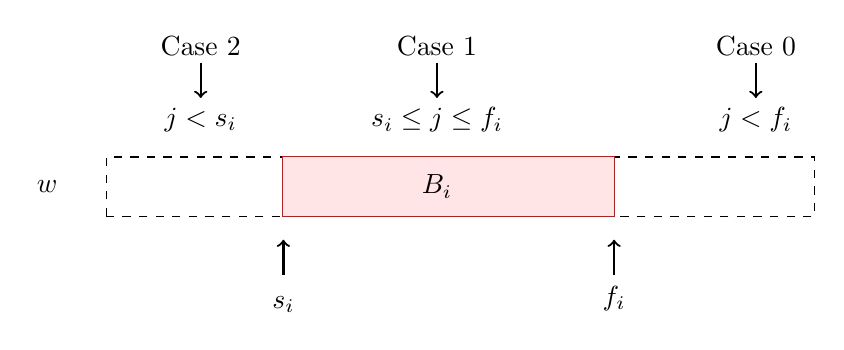
\begin{tikzpicture}[scale=1.5]
        % Main Rectangle w
        \draw[dashed] (0,0) rectangle (6,0.5);
        \node at (-0.5, 0.25) {\(w\)};

        % Smaller Rectangle 1 - Border color red
        \draw[draw=red, thick] (1.5,0) rectangle (4.3,0.5);
        
        \draw[->, thick] (1.5,-0.5) -- (1.5,-0.2);
        \node[align=center, below] at (1.5,-0.6) {\(s_{i}\)};
        \fill[red!10] (1.5,0) rectangle (4.3,0.5);
        \node at (2.8,0.25) {$B_{i}$};
        
        \draw[->, thick] (4.3,-0.5) -- (4.3,-0.2);
        
        \node at (4.3,-0.7) {$f_i$};
        
        
        \draw[->, thick] (5.5,1.3) -- (5.5,1);        
        \node[align=center, below] at (5.5,1) {\( j<f_i\)};
        \node[align=center, below] at (5.5,1.6) { \text{Case 0}};

        \draw[->, thick] (2.8,1.3) -- (2.8,1);        
        \node[align=center, below] at (2.8,1) {\( s_i \leq j \leq f_i\)};
        \node[align=center, below] at (2.8,1.6) {\text{Case 1}};

        \draw[->, thick] (0.8,1.3) -- (0.8,1);        
        \node[align=center, below] at (0.8,1) {\( j<s_i\)};
        \node[align=center, below] at (0.8,1.6) {\text{Case 2}};
        


    \end{tikzpicture}
    \caption{Compression for $w$ where $j$ is located.}
    \label{fig:case0}
\end{figure}


% So then, for case 0 $f_i<j$, it means that $s_i=s'_i$ and $f_i=f'_i$, LZ77 algorithm produces the exactly same result for $w[1,...,f_i]=w'[1,...,f_i]$, therefore. $B'_i$ is the only block that starts inside $B_i$, indeed, furthermore, $B_k=B'_k \forall k \leq i$.
% conclude that $f_i'\geq j$. When the case 1 holds, If $s_i\leq j\leq f_i$. We firstly have when $s_i=s'_i$, so that $B_k=B'_k \forall k \leq i-1$, this implies that $f_{i-1}=f'_{i-1}$. Hence $s_i=f_{i-1}+1 = f'_{i-1}+1 = s'_i$. We secondly have $f'_i\geq j$, so then, LZ77 compression only changes when a character is unknown for the string, thus, compression for $w'$ in the block $B'_i$ ends when $f_i=j$, moreover could be even greater, we never can finish before the index $j$ since compression up to $j$ is the same, so $|\mathcal{M}_i|= 1$ or $|\mathcal{M}_i|= 2$. Moreover, when $f'_{i+1}\geq f_i$, since $f_i\geq j$ we basically know that $f_i>f'_{i+1}$ but it does not matter how further $f'_{i+1}$ goes, because LZ77 compression guarantees that we can copy a substring that are previously encode. this automatically means that $|\mathcal{M}_i|= 2$ that is our important fact. On the other hand, analysis for case 2 relies when $j<s_i$ but based on LZ77 compression, when $j$ is placed before where the string for the block is copied over, it means that any place is located at compression for $w'$ adds at least 1 more block $B'_t$ that starts inside $B_k$ however since the condition holds we know that $f_i>f'_{i+1}$ therefore $|\mathcal{M}_i| \leq 2$.
% \end{proof}

% %%%%%%%%%%%%%%%%%%%%%%

% Let $t$ the maximum number of blocks after compressing $w'$ that \emph{Start Inside} $w$, since $w \sim w'$, then there is always a compression $(B'_1,...,B'_t)$ such as, WLOG $t'\geq t$ therefore, we defined $t'= \sum_{i=1}^{\infty}|\mathcal{M}_i|$, and $t= \sum_{i=1}^{\infty}|\mathcal{M}_i|$. These calculations are required for determine the quantity of blocks that \emph{Start Inside} either $B$ or $B'$ as a quantified property. Based on this reasoning and \defref{def:local_sensitivity} we introduce the difference to obtain Global Sensitivity, so then formally \claimref{claim:set:blocksm2:GS} as:
% %%%%%%%%%%%%%%%%%%%%%%%






% \lemblocknumupperbound

% \begin{proof}
%         If $i\in\B_2$ then either (1) $s_i\leq j\leq f_i$ or (2) $j-\ell_i < q_i \leq j$. When $j >f_i$, by LZ77 compression $B_i=B'_i$, thus $|\mathcal{M}_i|= 1$ and $i \in \mathcal{B_1}$.Hence, we have $s_i\leq j\leq f_i$ if $j\geq s_i$.
    
%     On the other hand, If $j<s_i$, then we want to show that $j-\ell_i<q_i\leq j$, i.e., $q_i\leq j < q_i+\ell_i$.
%     % \input{../Manuscript/figures/fig:claim9:case2}
%     Suppose for contradiction that $j\not\in[q_i,q_i+\ell_i-1]$.
%     Let $k$ be the smallest element in $\M_i$, i.e., $s_i\leq s_k'\leq f_i$ but $s_{k-1}'<s_i$.         
%     If $s_k'=f_i$, then if there is another $k'\in\M_i$ with $k'\neq k$, then by choice of $k$, we have $k<k'$ and therefore $s_{k'}'>f_k'>s_k'=f_i$. Hence, $|\M_i|= 1$ and $i\in\B_1$. Contradiction! It happens with any case for $j\not\in[q_i,q_i+\ell_i-1]$, since $i \in \B_2$. 
    
%     Now based on this, we are sure If $i_1,i_2\in\B_2$ then $(q_{i_1},\ell_{i_1})\neq(q_{i_2},\ell_{i_2})$. Since $i_1<i_2$ we then have $j<s_{i_1}<s_{i_2}$. Let $B_{i_1}=[q_{i_1},\ell_{i_1},c_{i_1}]$ and $B_{i_2}=[q_{i_2},\ell_{i_2},c_{i_2}]$ be  the blocks $B_{i_1}$ and $B_{i_2}$ of the LZ77 compression function $\compress:(\Sigma)^*\rightarrow(\Sigma')^*$ (Resp. w'). By intuition we know that there is no possibility to start in the same point for both Blocks $B_{i_1}$ and $B'_k$ after being read $j$ previously.
    

%     Finally Let $\B_2^\ell\coloneqq\{i\in\B_2:\ell_i=\ell\}$ and suppose that $s_{i^*}\leq j\leq f_{i^*}$ for some $i^*\in[t]$. Then $|\B_2^\ell|\leq\ell$ for all $\ell\neq \ell_{i^*}$, and $|\B_2^{\ell_{i^*}}|\leq\ell_{i^*}+1$. Furthermore, we observe that the constraint about length is: $\sum_{i\in\B_2} (\ell_i+1)\leq n,$ and $    \sum_\ell x_\ell'(\ell+1) < \sum_\ell x_\ell  (\ell+1) \leq n$. To find the threshold $z$, we observe that
% $\sum_{\ell=0}^z \ell(\ell+1) = \frac{1}{3}z(z+1)(z+2)\leq n,$
% which implies $z^3\leq 3n$ and $z\leq\sqrt[3]{3n}$. Setting this value of $z$, we have $t_2 \leq \frac{\sqrt[3]{9}}{2} n^{2/3} + \frac{\sqrt[3]{9}}{2} n^{1/3} + 1,$.
% \end{proof}

% The main result of this subsection is based on the analysis for upper bounding the global sensitivity, so then, in \secref{sec:upperbound} the goal is to provide the exact coefficient for the bound as is shown in the following theorem:




\section{Lower Bound for the Global Sensitivity of LZ77 Compression}\seclab{sec:lowerbound}

% =====

% \paragraph*{String Construction for the GS Lower Bound.}

% To prove the lower bound $\Omega(n^{2/3}\log^{1/3}n)$ for the global sensitivity of the LZ77 compression, we need to give example strings $w\sim w'$ of length $n$ that achieves $\left||\compress(w)|-|\compress(w')|\right|=\Omega(n^{2/3}\log^{1/3} n)$ (where $\compress$ denotes the LZ77 compression function) since this implies
% \begin{align*}
%     \mathtt{GS}_{\mathtt{Compress}} &= \max_{x \in \Sigma^n} \mathtt{LS}_{\mathtt{Compress}}(x)\\
%     &= \max_{x \in \Sigma^n}\max_{x' \in \Sigma^n:x\sim x'} \left| |\compress(x)| - |\compress(x')| \right|\\
%     &\geq \left||\compress(w)|-|\compress(w')|\right|\\
%     &=\Omega(n^{2/3}\log^{1/3} n).
% \end{align*}
% We give strings $w\sim w'$ that are carefully crafted such that $|w|=|w'|=\Theta(m^3\log m)$ for some integer $m>0$ and the number of type-2 blocks is $\Theta(m^2)$, which implies that $\GS_\compress=\Omega(m^2\log m) = \Omega(n^{2/3}\log^{1/3}n)$ where $n=\Theta(m^3\log m)$ denotes the length of strings. A core component of the string construction is to consider an \emph{injective encoding} of the number set $[m]$, which takes $\lceil\log m\rceil$ bits for each encoding, to ensure that each encoding is unique. This helps us count the number of type-2 blocks. However, having an injective encoding only does not fully resolve the issue 

% We overcome this bottleneck by \emph{repeating} each encoding twice.

% =====

In \secref{sec:upperbound}, we proved that the upper bound for the global sensitivity of the LZ77 compression algorithm $\compress$ is $O(n^{2/3}\log n)$ with window size $W=n$. One could ask if this is a tight bound, i.e., if we can prove the matching \emph{lower bound} for the global sensitivity of $\compress$ as well. This section proves the almost-matching lower bound up to a sub-logarithmic factor. In particular, we show that the global sensitivity of the LZ77 compression algorithm is $\Omega(n^{2/3}\log^{1/3} n)$. To prove the lower bound, we need to give example strings $w\sim w'$ of length $n$ that achieves $\left||\compress(w)|-|\compress(w')|\right|=\Omega(n^{2/3}\log^{1/3} n)$ since this implies $\GS_\compress=\max_{x \in \Sigma^n}\max_{x' \in \Sigma^n:x\sim x'} \left| |\compress(x)| - |\compress(x')| \right|\geq \left||\compress(w)|-|\compress(w')|\right|=\Omega(n^{2/3}\log^{1/3} n)$. 
% \begin{align*}
%     \mathtt{GS}_{\mathtt{Compress}} &= \max_{x \in \Sigma^n}\max_{x' \in \Sigma^n:x\sim x'} \left| |\compress(x)| - |\compress(x')| \right|\\
%     &\geq \left||\compress(w)|-|\compress(w')|\right|=\Omega(n^{2/3}\log^{1/3} n).
% \end{align*}
For the rest of \secref{sec:lowerbound}, we will give the construction of such example strings $w$ and $w'$.

\subsection{String Construction}

Consider an encoding function $\Enc:\mathbb{Z}\rightarrow\bin^*$ that maps integers to binary strings. Then for a positive integer $m\in\mathbb{Z}$, we have an injective encoding of the number set $\mathcal{S}\coloneqq\left\{0,1,\ldots, m\right\}$ using $\lceil\log m\rceil$ bits, i.e., $\Enc(i)\neq\Enc(j)$ if $i,j\in\mathcal{S}$ and $i\neq j$. For example, if $m=2^q-1$ for some positive integer $q$, we could encode the elements of $\S$ as follows: 
\[\Enc(0)=0^{\lceil\log m\rceil},\Enc(1)=0^{\lceil\log m\rceil-1}1,\Enc(2)=0^{\lceil\log m\rceil-2}10,\ldots,\Enc(m)=1^{\lceil\log m\rceil}.\] 
Now, consider a quinary alphabet $\Sigma=\{0,1,2,3,4\}$ and define a string
\[S_{\ell,u}\coloneqq\Enc(m-u+1)^2\circ\Enc(m-u+2)^2\circ\cdots\circ\Enc(m)^2\circ 2 \circ\Enc(m+1)^2\circ\cdots\circ\Enc(m-u+\ell)^2 \]
in $\Sigma^*$ for $2\leq\ell\leq m$ and $1\leq u\leq\ell-1$. 
Here, $(\cdot)^2$ denotes the concatenation of the string itself twice, i.e., $\Enc(\cdot)^2=\Enc(\cdot)\circ\Enc(\cdot)$. 
We define a procedure called $\QuinStr(m)$ which takes as input a positive integer $m\in\mathbb{Z}$ and outputs two quinary strings as follows.

\begin{tcolorbox}[breakable,enhanced,title={The Construction of Two Quinary Strings $\QuinStr(m)$.}]
    \begin{enumerate}
        \item The algorithm computes two quinary strings $S_w$ and $S_{w'}$ where
        \begin{align*}
            S_w &\coloneqq\Enc(1)^2\circ\cdots\circ\Enc(m)^2\circ 2 \circ\Enc(m+1)^2\circ\cdots\circ\Enc(2m)^2\circ 4,\text{ and}\\
            S_{w'} &\coloneqq\Enc(1)^2\circ\cdots\circ\Enc(m)^2\circ 3 \circ\Enc(m+1)^2\circ\cdots\circ\Enc(2m)^2\circ 4.
        \end{align*}
        \item Then it computes two quinary strings $w,w'$ defined as $w\coloneqq S_w\circ S$ and $w'\coloneqq S_{w'}\circ S$, where
        \[S = S_{2,1} \circ 4 \circ S_{3,2} \circ 4 \circ S_{3,1} \circ 4 \circ \ldots \circ S_{m,m-1} \circ 4 \circ \ldots \circ S_{m,1}\circ 4.\]
        \item Output $(w,w')$.
    \end{enumerate}
\end{tcolorbox}

\claimref{claim:length} tells us that the strings $w$ and $w'$ outputted by the procedure $\QuinStr(m)$ has equal length $\Theta(m^3\log m)$. Since the proof is elementary, we defer the proof of \claimref{claim:length} to \appref{app:missingprooflowerbound}.

\newcommand{\claimlength}{
Let $m\in\mathbb{N}$ and $(w,w')\gets\QuinStr(m)$. Then $|w|=|w'|=\Theta(m^3\log m)$. In particular, for $m\geq 4$, $\frac{2}{3}m^3\lceil\log m\rceil< |w|=|w'|< m^3\lceil\log m\rceil$.
}
\begin{claim}\claimlab{claim:length}
\claimlength
\end{claim}

\subsection{Analyzing the Sensitivity of $\QuinStr(m)$}

A central step in our sensitivity analysis for $\QuinStr(m)$ is precisely counting the type-2 blocks produced by the LZ77 compression scheme, as we observed in \secref{sec:upperbound}. \lemref{lem:gs} shows that for $(w,w')\gets\QuinStr(m)$, we have $|\B_2|=\frac{(m-1)m}{2}-(\lfloor\frac{m}{2}\rfloor-1)$. Intuitively, we first show that for $w=S_w\circ S$, there is no type-2 block for the blocks compressing $S_w$. Then the main insight is that we carefully crafted strings $w$ and $w'$ such that the marker symbol `4' becomes the endpoint for each block in $\compress(w)$ for the tail part $S$ of $w=S_w\circ S$. By repeating each encoding twice, we can ensure that most of the occurrences of $S_{\ell,u}\circ 4$ yield type-2 blocks, with an edge case (addressed in \claimref{claim:repeat}) that makes the block in $\B_1$ but this happens for only about $m/2$ blocks. Consequently, despite these few exceptions, the overall count of type-2 blocks remains quadratic in $m$.

\newcommand{\lemGS}{
Let $m\in\mathbb{N}$ and $(w,w')\gets\QuinStr(m)$ and let $\compress:\Sigma^*\rightarrow(\Sigma')^*$ be the LZ77 compression algorithm. Let $(B_1,\ldots,B_t)\gets\compress(w)$ and $(B'_1,\ldots,B'_{t'})\gets\compress(w')$. Then $|\B_0| = 0$ and $|\B_2| = \frac{(m-1)m}{2}-(\lfloor\frac{m}{2}\rfloor-1)$.
}
\begin{lemma}\lemlab{lem:gs}
    \lemGS
\end{lemma}

\begin{proof}
Recall that $w = S_w \circ S$ and $w' = S_{w'} \circ S$, where
\begin{itemize}
    \item $S_w =\Enc(1)^2\circ\cdots\circ\Enc(m)^2\circ 2 \circ\Enc(m+1)^2\circ\cdots\circ\Enc(2m)^2\circ 4$,
    \item $S_{w'}=\Enc(1)^2\circ\cdots\circ\Enc(m)^2\circ 3 \circ\Enc(m+1)^2\circ\cdots\circ\Enc(2m)^2\circ 4$, and
    \item $S=S_{2,1} \circ 4 \circ S_{3,2} \circ 4 \circ S_{3,1} \circ 4 \circ \ldots \circ S_{m,m-1} \circ 4 \circ \ldots \circ S_{m,1}\circ 4$, where
    \item $S_{\ell,u}\coloneqq\Enc(m-u+1)^2\circ\Enc(m-u+2)^2\circ\cdots\circ\Enc(m)^2\circ 2 \circ\Enc(m+1)^2\circ\cdots\circ\Enc(m-u+\ell)^2$ for $2\leq\ell\leq m$ and $1\leq u\leq \ell-1$.
\end{itemize}
We first observe that $w\sim w'$. Define $S_w^F\coloneqq \Enc(1)^2\circ\cdots\circ\Enc(m)^2\circ 2$ (resp. $S_{w'}^F\coloneqq \Enc(1)^2\circ\cdots\circ\Enc(m)^2\circ 3$) to be the first-half substring of $S_w$ (resp. of $S_{w'}$), and $S_w^L=S_{w'}^L\coloneqq \Enc(m+1)^2\circ\cdots\circ\Enc(2m)^2\circ 4$ to be the last-half substring of $S_w$ (or $S_{w'}$ since they are indeed identical). 
It is useful to define a notation $\str(B_k)$ for a block $B_k$, which denotes the substring of $w$ represented by the block $B_k$, i.e., for $B_k=[q_k,\ell_k,c_k]$, $\str(B_k)\coloneqq w[q_k,q_k+\ell_k-1]\circ c_k$. 

Let $B_{i_1}$ be the first block such that $S_w^F$ becomes a substring of $\str(B_1)\circ\str(B_2)\circ\ldots\circ\str(B_{i_1})$, and similarly, let $B'_{i'_1}$ be the first block such that $S_{w'}^F$ becomes a substring of $\str(B'_1)\circ\str(B'_2)\circ\ldots\circ\str(B'_{i'_1})$. Then we observe the following:
\begin{enumerate}
    \item $B_{i_1}=[q_{i_1},\ell_{i_1},2]$, i.e., $\str(B_{i_1})$ ends with $2$ (which is the last character in $S_w^F$), since $2$ never showed up before as all the encodings are binary strings, it has to be added to the dictionary as a new character,
    \item $B_i=B_i'$ for all $i\in[i_1-1]$, as we are compressing the identical strings until we see $2$ in $S_w^F$ (and $3$ in $S_{w'}^F$), and
    \item $i_1=i_1'$ and $B'_{i_1}=[q_{i_1},\ell_{i_1},3]$, since two strings $S_w^F$ and $S_{w'}^F$ are identical except for the very last character.\label{item:2}
\end{enumerate}

Now let $B_{i_2}$ be the first block such that $S_w^L$ becomes a substring of $\str(B_{i_1+1})\circ\str(B_{i_1+2})\circ\ldots\circ\str(B_{i_2})$, and similarly, let $B'_{i'_2}$ be the first block such that $S_{w'}^L$ becomes a substring of $\str(B'_{i_1+1})\circ\str(B'_{i_1+2})\circ\ldots\circ\str(B'_{i'_2})$. Then we observe the following:
\begin{enumerate}
\setcounter{enumi}{3}
    \item $i_2=i_2'$ and $B_i=B_i'$ for all $i\in[i_1+1,i_2]$, since $i_1=i_1'$ from observation \ref{item:2} and we have $S_w^L=S_{w'}^L$ while they do not contain $2$ or $3$, and
    \item $B_{i_2}=[q_{i_2},\ell_{i_2},4]$, since $4$ never showed up before in our compression.
\end{enumerate}

From the observations above, we have that $B_i\in\B_1$ for all $i\in[i_2]$. 
Now we are left with the blocks $(B_{i_2+1},\ldots,B_t)$ compressing the last part $S$ of $w$ and the blocks $(B'_{i_2+1},\ldots,B'_{t'})$ compressing the last part $S$ of $w'$. For the blocks $(B_{i_2+1},\ldots,B_t)$, we observe that each block ends at the next `$4$' because each $S_{\ell,u}$ (for $2\leq\ell\leq m$ and $1\leq u\leq \ell-1$) is contained in the former part of $w$ (which was $S_w$) but $4$ only shows up in $S_w$ followed by $\Enc(2m)^2$ while $S_{\ell,u}$ cannot contain $\Enc(2m)$. Hence, we observe the following:
\begin{enumerate}
\setcounter{enumi}{5}
    \item $\str(B_{i_2+1})=S_{2,1}\circ 4,\str(B_{i_2+2})=S_{3,2}\circ 4$,  and so on.
    \item In general, $\str\left(B_{i_2+\frac{(\ell-2)(\ell-1)}{2}+(\ell-t)}\right)=S_{\ell,u}\circ 4$, for $2\leq\ell\leq m$ and $1\leq u\leq \ell-1$. This indeed covers all the blocks from $B_{i_2+1},\ldots,B_t$ (See \claimref{claim:inj} and observation \ref{item:8}).
    \item Furthermore, we can observe that $t= i_2 + (1+2+\ldots+(m-1)) = i_2 + \frac{(m-1)m}{2}$.\label{item:8}
\end{enumerate}

\newcommand{\felluinjective}{
For any integer $m\geq 2$, the function $f(\ell,u)\coloneqq\frac{(\ell-2)(\ell-1)}{2}+(\ell-u)$ defined over integers $\ell$ and $u$ such that $2\leq \ell\leq m$ and $1\leq u\leq \ell-1$ is injective, and its range is $[\frac{(m-1)m}{2}]$.
}
\begin{claim}\claimlab{claim:inj}
\felluinjective
\end{claim}

The proof of \claimref{claim:inj} is elementary by induction on $m$, and hence, we defer the proof to \appref{app:missingprooflowerbound}. What we are interested in is whether each $B_i$, for $i_2+1\leq i\leq t$, belongs to $\B_0$, $\B_1$, or $\B_2$. In \claimref{claim:blocks}, we prove that the blocks are mostly in $\B_2$ and the rest of the blocks are in $\B_1$, meaning that $\B_0=\emptyset$. In particular, we prove that for $2\leq\ell\leq m$ and $1\leq u\leq\ell-1$, $B_{i_2+\frac{(\ell-2)(\ell-1)}{2}+(\ell-u)}\in\B_1$ if and only if all of these conditions hold: (1) $\ell>2$, (2) $\ell$ is even, and (3) $u=\ell/2$. 

\begin{claim}\claimlab{claim:blocks}
For $2\leq\ell\leq m$ and $1\leq u\leq \ell-1$, $B_{i_2+\frac{(\ell-2)(\ell-1)}{2}+(\ell-u)}\in\B_1$ if and only if $\ell>2, 2\mid\ell$, and $u=\ell/2$; otherwise $B_{i_2+\frac{(\ell-2)(\ell-1)}{2}+(\ell-u)}\in\B_2$.
%For $\ell'\in\left[\lfloor\frac{m}{2}\rfloor\right]$, $B_{i_2+(\ell'-1)(2\ell'-1)+\ell'}\in\B_1$ and 
\end{claim}

We will give the proof of \claimref{claim:blocks} below and finish the proof of \lemref{lem:gs} first for readability. By \claimref{claim:blocks}, since there are only $\lfloor\frac{m}{2}\rfloor-1$ of such pairs of $(\ell,u)$, we observe that $|\B_2|=\frac{(m-1)m}{2}-(\lfloor\frac{m}{2}\rfloor-1)$. Since we have that $B_i\in\B_1$ for all $i\in[i_2]$, we have $\B_0=\emptyset$ and therefore $|\B_0|=0$. This completes the proof of \lemref{lem:gs}.
\end{proof}

\begin{proofof}{\claimref{claim:blocks}}
Recall that $S=S_{2,1}\circ4\circ S_{3,2}\circ4\circ S_{3,1}\circ4\circ\ldots\circ S_{m,m-1}\circ4\circ\ldots\circ S_{m,1}\circ4$ and $\str(B_{i_2+1})=S_{2,1}\circ4$, $\str(B_{i_2+2})=S_{3,2}\circ4$, $\str(B_{i_2+3})=S_{3,1}\circ4,\ldots,\str(B_t)=S_{m,1}\circ4$. 
For each $S_{\ell,u}$, we observe that $S_{\ell,u}$ is \emph{not} a substring of $S_{w'}$. Hence, we see that each block $B_i$ (for $i_2+1\leq i\leq t$) is roughly split into two blocks for the blocks of $\compress(w')$ unless it could copy beyond the character $4$. To observe the cases when this happens,
for each $S_{\ell,u}$, it is helpful to define:
\begin{itemize}
    \item $S_{\ell,u}^F\coloneqq\Enc(m-u+1)^2$ denotes the very first encoding concatenation that shows in $S_{\ell,u}$, 
    \item $S_{\ell,u}^{F,(1/2)}\coloneqq\Enc(m-u+1)$ denotes the very first encoding in $S_{\ell,u}$ (i.e., half of $S_{\ell,u}^F$),
    \item $S_{\ell,u}^L\coloneqq\Enc(m-u+\ell)^2$ denotes the very last encoding concatenation that shows in $S_{\ell,u}$, and
    \item For $k>u$, $S_{\ell,u}^{(k)}\coloneqq\Enc(m-u+1)^2\circ\Enc(m-u+2)^2\circ\ldots\circ\Enc(m)^2\circ2\circ\Enc(m+1)^2\circ\ldots\circ\Enc(m-u+k)^2$ denotes the first $k$ encoding concatenations that shows in $S_{\ell,u}$.
\end{itemize}
Then we observe the following claims. Since proofs of \claimref{claim:notrepeat} and \claimref{claim:repeat} are elementary, we defer the proofs to \appref{app:missingprooflowerbound}.

\begin{claim}\claimlab{claim:notrepeat}
$S_{\ell,u}^L\circ4\circ S_{\ell,u-1}^F$ does not repeat for different $\ell$ and $u$ such that $3\leq\ell\leq m$ and $2\leq u\leq\ell-1$.
\end{claim}

\claimref{claim:notrepeat} tells us that, due to the injectivity of the encoding, any block in $\compress(w')$ containing a portion of $S_{\ell,u}^L$ along with the delimiter `4' must finish at $S_{\ell,u}^{F,(1/2)}$ in the worst case. In particular, note that $S_{\ell,u}^L=\Enc(m-u+\ell)^2=S_{\ell+1,u+1}^L$ for $3\leq \ell<m$ and $2\leq u<\ell-1$. Moreover, we have $S_{\ell,u-1}^{F,(1/2)}=\Enc(m-u+2)$ and $S_{\ell+1,u}^{F,(1/2)}=\Enc(m-u+1)$, which can agree on all but the final bit (e.g., $S_{\ell,u-1}^{F,(1/2)}=00\cdots00$ and $S_{\ell+1,u}^{F,(1/2)}=00\cdots01$). Without the repetition of each encoding, a block might incorporate nearly the entire $S_{\ell+1,u}^{F,(1/2)}$ except for the last bit. Consequently, by having this last bit as a new character, $S_{\ell,u-1}\circ4$ would be placed in $\B_1$. Repeating the encoding twice eliminates this possibility and we can ensure that the scenario described in \claimref{claim:repeat} is the only case where type-1 blocks would occur. Again, see \appref{app:missingprooflowerbound} for the proof of \claimref{claim:repeat}.


\begin{claim}\claimlab{claim:repeat}
For $2\leq\ell\leq\lfloor\frac{m}{2}\rfloor-1$, $S_{\ell,1}^L\circ4\circ S_{\ell+1,\ell}$ repeats at $S_{2\ell,\ell+1}^L\circ4\circ S_{2\ell,\ell}^{(\ell+1)}$.
\end{claim}

Let's go back to the proof of \claimref{claim:blocks}. By \claimref{claim:repeat}, we can see that the block of the form $B_{i_2+\frac{(2\ell-2)(2\ell-1)}{2}+(2\ell-\ell)}$ which satisfies
\[\str\left(B_{i_2+\frac{(2\ell-2)(2\ell-1)}{2}+(2\ell-\ell)}\right)=S_{2\ell,\ell}\circ4,\]
is in $\B_1$, and all of the other blocks beyond $B_{i_2}$ are in $\B_2$. This completes the proof of \claimref{claim:blocks}.
% We first observe the following.
% Now, let's analyze the blocks $(B'_{i_2+1},\ldots,B'_{i'_3})$. Consider $B'_{i_2+1}$ first as a warmup. Recall that $\str(B_{i_2+1})=S_{2,1}\circ 4$ because $S_{2,1}=\Enc(m)^2\circ 2\circ \Enc(m+1)^2$ was a substring of $S_w$, but this is \emph{not} the case for $w'$ since we replaced $2$ with $3$ in $S_{w'}$. This observation implies that $\str(B'_{i_2+1})=\Enc(m)^2\circ 2$ (which is the substring of $S_{2,1}$) since $\Enc(m)^2$ was contained in $S_{w'}$ and it is indeed the longest substring you could copy from the prior substring since $2$ never showed up in $w'$.
% Next, consider the next block $B'_{i_2+2}$. It is easy to see that $\str(B'_{i_2+2})=\Enc(m+1)^2\circ 4$ because $\Enc(m+1)^2$ is a substring of $S_{w'}$ and $4$ only showed up once in a prior substring, followed by $\Enc(2m)^2$ (in $S_{w'}\circ 4$). With a similar argument, we observe that $\str(B'_{i_2+3})=\Enc(m-1)^2\circ\Enc(m)^2\circ 2$ (which is a substring of $S_{3,2}$). Now for the block $B'_{i_2+4}$, one might think that $\str(B'_{i_2+4})=\Enc(m+1)^2\circ 4\circ c'_{i_2+4}$ where $c'_{i_2+4}$ is the first character in $\Enc(m)$ (since $S_{3,1}$ starts with $\Enc(m)^2$) since it seems to be the case that $\Enc(m+1)^2\circ 4$ is the longest substring of $S_{w'}\circ 4 \circ S_{2,1}\circ 4\circ \Enc(m-1)^2\circ\Enc(m)^2\circ 2$
\end{proofof}

Taken altogether, we can lower bound the global sensitivity of the LZ77 compression scheme as stated in \thmref{thm:lowerbound} below.

\begin{theorem}\thmlab{thm:lowerbound}
Let $\compress:\Sigma^*\rightarrow\Sigma'^*$ be the LZ77 compression function. Then $\mathtt{GS}_\compress\geq 4^{-1/3}\cdot n^{2/3}\log^{1/3}n=\Omega(n^{2/3}\log^{1/3}n)$. 
\end{theorem}

\begin{proof}
Let $(w,w')\gets\QuinStr(m)$ and let $|w|=|w'|=n$. By \claimref{claim:length}, we have $|w|=|w'|=\Theta(m^3\log m)$ and therefore $n=\Theta(m^3\log m)$. Furthermore, \claimref{claim:length} tells us that there exists some $\alpha$ with $\frac{2}{3}\leq\alpha\leq 1$ such that $n=\alpha m^3\log m$.  
Now let $(B_1,\ldots,B_t)\gets\compress(w)$ and $(B'_1,\ldots,B'_{t'})\gets\compress(w')$.
Recall that if we look at the proof of \claimref{claim:set:blocksm2:GS}, it tells us that $t'-t=|\B_2|-|\B_0|$. From \lemref{lem:gs}, we have $|\B_0|=0$ and $|\B_2|=\frac{(m-1)m}{2}-(\lfloor\frac{m}{2}\rfloor-1)$, which implies that $t'-t=\frac{(m-1)m}{2}-(\lfloor\frac{m}{2}\rfloor-1)$. We know $|\compress(w)|=t(2\lceil\log n\rceil+\lceil\log|\Sigma|\rceil)$ and $|\compress(w')|=t'(2\lceil\log n\rceil+\lceil\log|\Sigma|\rceil)$, we have
\begin{align*}
   \mathtt{GS}_{\mathtt{Compress}} & \leq  \left||\compress(w)|-|\compress(w')|\right|  
   = |t-t'|\left(2\lceil\log n\rceil+\lceil\log|\Sigma|\rceil\right) \\
    &= |t-t'|\left(2\left\lceil\log (\alpha m^3\log m)\right\rceil+\lceil\log|\Sigma|\rceil\right) 
    %\geq \left[\frac{(m-1)m}{2}-\left(\left\lfloor\frac{m}{2}\right\rfloor-1\right)\right]\cdot2\log(\alpha m^3\log m)\\
    \geq \frac{m^2}{4}\cdot 4\log m = m^2\log m \ .
\end{align*}
% \begin{align*} backup for full version
%     \left||\compress(w)|-|\compress(w')|\right| &= |t-t'|\left(2\lceil\log n\rceil+\lceil\log|\Sigma|\rceil\right) \\
%     &= |t-t'|\left(2\left\lceil\log (\alpha m^3\log m)\right\rceil+\lceil\log|\Sigma|\rceil\right)\\
%     &\geq \left[\frac{(m-1)m}{2}-\left(\left\lfloor\frac{m}{2}\right\rfloor-1\right)\right]\cdot2\log(\alpha m^3\log m)\\
%     &\geq \left(\frac{m^2}{2}-m\right)\cdot 4\log m\\
%     &\geq \frac{m^2}{4}\cdot 4\log m = m^2\log m,
% \end{align*}
%which implies that
%\begin{align*}
 %   \mathtt{GS}_{\mathtt{Compress}} &= \max_{x \in \Sigma^n}\max_{x' \in \Sigma^n:x\sim x'} \left| |\compress(x)| - |\compress(x')| \right|\\
 %   &\geq \left||\compress(w)|-|\compress(w')|\right|\\
  %  &= m^2\log m.
%\end{align*}
Furthermore, since we have $n=\alpha m^3\log m$ for some $\frac{2}{3}\leq\alpha\leq 1$, we observe that
\begin{align*}
    m^2\log m &= m^2\cdot\frac{n}{\alpha m^3}= \frac{n}{\alpha}\cdot\frac{1}{m} = \frac{n}{\alpha}\cdot\frac{\alpha^{1/3}\cdot\log^{1/3}m}{n^{1/3}}
    \geq \left(\frac{n}{\alpha}\right)^{2/3}\cdot 4^{-1/3}\cdot\log^{1/3}n \\
    &\geq 4^{-1/3}\cdot n^{2/3}\log^{1/3}n,
\end{align*}
% \begin{align*} backup for full version
%     m^2\log m &= m^2\cdot\frac{n}{\alpha m^3}\\
%     &= \frac{n}{\alpha}\cdot\frac{1}{m}\\
%     &= \frac{n}{\alpha}\cdot\frac{\alpha^{1/3}\cdot\log^{1/3}m}{n^{1/3}}\\
%     &= \left(\frac{n}{\alpha}\right)^{2/3}\cdot\log^{1/3}m\\
%     &\geq \left(\frac{n}{\alpha}\right)^{2/3}\cdot 4^{-1/3}\cdot\log^{1/3}n\\
%     &\geq 4^{-1/3}\cdot n^{2/3}\log^{1/3}n,
% \end{align*}
where the first inequality comes from the observation $\log n = \log\alpha + 3\log m + \log\log m\leq 4\log m$ and the second inequality comes from $(1/\alpha)\geq 1$. Hence,
\begin{align*}
    \mathtt{GS}_{\mathtt{Compress}} &\geq m^2\log m \geq 4^{-1/3}\cdot n^{2/3}\log^{1/3}n,
\end{align*}
% Since we know $\frac{2}{3}\cdot m^3\log m\leq n\leq m^3\log m$ from \claimref{claim:length}, we observe that 
% \begin{align*}
%     m^2\log m &= \frac{1}{m}\cdot m^3\log m\\
%     &\geq \frac{1}{m}\cdot n\\
%     &\geq \sqrt[3]{\frac{2}{3}}\cdot n^{-1/3}\cdot\left(\log^{1/3}m\right)\cdot n\\
%     &\geq \sqrt[3]{\frac{2}{3}}\cdot n^{-1/3}\cdot\left(\sqrt[3]{\frac{1}{6}}\cdot\log^{1/3}n\right)\cdot n\\
%     &= \sqrt[3]{\frac{1}{9}}\cdot n^{2/3}\log^{1/3}n,
% \end{align*}
% where the third inequality is achieved by the observation that $3\log m\geq \log n - \log\log m \geq \frac{\log n}{2}$, since $\log m\leq \sqrt{n}$.
% Hence,
% \begin{align*}
%     \mathtt{GS}_{\mathtt{Compress}} &\geq m^2\log m\\
%     &\geq \sqrt[3]{\frac{1}{9}}\cdot n^{2/3}\log^{1/3}n,
% \end{align*}
which completes the proof.
\end{proof}

\section{Adversarial example generation}
\section{Application: Harnessing the Linearity}
\label{sec:application}
Leveraging the \emph{linearity} of DMD operator, as well as the intuition of bases exposed by the spectral decomposition, we have developed several novel applications that extend the capabilities of our Koopman-based reduced-order simulation pipeline. In this section, we explore these applications, demonstrating that our method's unique strengths translate into practical tools for graphics and simulation.

\subsection{Direct Editing Temporal Dynamics}
\label{sec:editing}
\begin{figure}[!ht]
    \centering
    \includegraphics[width=1\columnwidth]{figure/karman_vortex_street_editing.pdf}
    \caption{\textbf{Editing temporal dynamics of K\'arm\'an Vortex Street with the Koopman Operator Approximation}. The modifications are applied to the DMD basis coefficients: (a) Scaling the modulus of the DMD basis by factors of 0.5, 1.0, and 1.5, affecting overall amplitude; (b) Adjusting the real part of $\bm{\Omega}$, influencing growth and decay rates of modal contributions; (c) Modifying the imaginary part, altering phase dynamics and wave propagation characteristics. }
    \label{fig:karman_editing}
    \Description{}
\end{figure}


\begin{figure*}[!ht]
    \centering
    \includegraphics[width=1\linewidth]{figure/reversibility.pdf}
    \caption{\textbf{Reversibility of Flows with Inversed DMD Operator}. We compare the reconstruction of two distinct fluid flows using Dynamic Mode Decomposition (DMD). The top row in each panel shows the velocity L2-norm of the field used to train the DMD, while the second and third rows depict the temporal evolution of the reconstructed flow fields as applied to an initial density field. The forward-time training phase is followed by a backward-time testing phase to assess predictive accuracy when advecting backward in time. The bottom plots show the evolution of kinetic energy over time. From the buoyant case, we observe the inverted DMD operator $\bm{A^{-1}}$ can still reasonably trace backward in time without compromising much visual quality. The vortical case exhibits a more challenging example where the symmetry should be reconstructed backwards in time. We see that the inverse operator indeed recovers this symmetry, with some acceptable levels of incurred noise. Bottom plots show the evolution of the total kinetic energy over time, demonstrating that our inverse operator actually correctly reverses the arrow of time, reversing the dissipation-related entropy increase over time. Decreasing kinetic energy also validates the \emph{physical plausibility} of our result.}
    \label{fig:reverse_simulation}
    \Description{}
\end{figure*}


Since our method approximates \refeq{eqn:euler_equations} with a linear operator in the full space, this allows us to transform the operator acting on the velocity field into the evolution of different modes under a linear operator. Therefore, we can directly edit the temporal dynamics of the fluid system by modifying the modes of the reduced \koopman{} $\bm{\hat{K}}$:
we set $t_0$ to be the initial time, $\bm{\Omega} = \nicefrac{\log(\bm\Lambda)}{\Delta t}$, where $\Delta t$ is the time step of the dataset. With this, we can rewrite \refeq{eqn:reduced_koopman_simulation} in the following form:
\begin{equation}
    \begin{aligned}
    \bm{u}(t_0 + k\Delta t) &= \bm{\Phi}\exp(\bm{\Omega} t) \bm{z}(t_0) \\
    &= \bm{\Phi}\exp{\left(k(\log(r) + i\theta)\right)} \bm{z}(t_0) \\
    &= \sum_{i = 1}^{n} {w_i} \bm{\Phi_i} r_i^k \left(\cos(k\theta_i) + \sin(k\theta_i)\right) \bm{z_i}(t_0)\\
    \end{aligned}
    \label{eqn:edit_temporal}
\end{equation}
% explanation for the formula
where ${w_i}$ is a user-defined scalar weight, $r_i = \sqrt{\Re(\lambda_i)^2 + \Im(\lambda_i)^2}$ is the \emph{modulus} and $\theta_i = \arctan\left(\Im(\lambda_i), \Re(\lambda_i)\right)$ is the \emph{phase} of the $i$-th eigenvalue $\lambda_i$ in the diagonal \emph{complex} eigenvalue matrix $\bm{\Lambda}$. Notice that this implies that the modes of the spectral decomposition represent different scales of vorticity, completing the physical intuition of the reduced space modes.
% show the benefits of our method for artist to edit

As shown in \refeq{eqn:edit_temporal}, our method decomposes a simulation sequence into modes with different growth/decay rates and frequencies.
The growth/decay rate of a mode is reflected in $r_i$, where a larger $r_i$ indicates a higher growth rate (or a lower decay rate), and vice versa.
The frequency of a mode is represented by the absolute value of $\theta_i$, with a larger absolute value corresponding to a higher frequency mode, and vice versa.
Furthermore, the different modes are decoupled, allowing for the adjustment of the relative proportions between modes.
As a result, these properties provide the artist with powerful tools to edit the simulation playback. The artist can modify the overall velocity field by adjusting the proportion ($w_i$), growth/decay rate ($r_i$), and frequency ($\theta_i$) of specific modes.
% explanation for what we actually do in code
In the experiments, we directly adjust the real part of $\bm{\Omega_i}$ to control $r_i$, modify the imaginary part of $\bm{\Omega_i}$ to control $\theta_i$, and vary the modulus of $\bm{\Phi_i}$ to control $w_i$.
% explanation for what we did to edit in karman vortex street scene
\paragraph{Editing the K\'arm\'an Vortex Street}
The first example is editing on the classic K\'arm\'an vortex street. We filter the imaginary part of $\bm{\Omega}$ and cluster modes with an absolute value smaller than $0.01$ as \emph{low-frequency cluster}, and the rest as \emph{high-frequency cluster}.
The low-frequency mode manifests as a laminar flow, with its phase changing very slowly over time. The high-frequency mode is represented by vortical structures distributed on both sides of the cylinder, where the phase of this mode changes relatively quickly over time.
As seen in \reffig{fig:karman_editing}, when we adjust the modulus of the high-frequency cluster from $0.5$ to $1.5$, the intensity of the vortices increases, which is as we expected. When we set the real part of $\bm{\Omega}$ to $0.5$, it can be observed that the high-frequency motion decays faster than user input. When we set the real part of $\bm{\Omega}$ to $1.5$, it can be observed that the high-frequency motion decays slower than user input. Similarly, when we tune the imaginary part of $\bm{\Omega}$ from $0.5$ to $1.5$, we could observe the oscillation frequency of the fluid trail transitions from slow to fast compared to user input.
% explanation for what we did to edit in 3D plume scene
\paragraph{Editing the Plume with Bunny}
To evaluate the editing capability of our method, we scale our editing scenario to 3D. With the same filtering procedure as in the K\'arm\'an vortex street example, we set the low-frequency cluster to high-frequency cluster ratio to $4:1$, $2:1$, $1:2$, and $1:4$, and compared the results with the user input. From the results, we observe that when the proportion of low-frequency cluster is increased, with a ratio of $4:1$, the top of the plume lacks "wrinkles" and appears more "fluffy". This is because the velocity field is dominated by smoother, lower-frequency modes than the original user input. Conversely, when the proportion of high-frequency cluster is increased, with ratios of $1:4$, the plume developes more detailed plume structure around the top, as the velocity field now emphasizes more high-frequency details compared to the user input.

\subsection{Reversibility of the Reduced Simulation}
Although physically-based fluid simulations have the capability to generate stunning visuals, when artists aim to direct the fluid's evolution toward a predefined target shape, challenges arise. It is a long standing problem in the community that people aim to enable users with \emph{spatial control}. In this example, we aim to enable users to do \emph{temporal control}, motived by a prior work \citet{oborn2018time}. Compared to previous work \shortcite{oborn2018time} where the authors employ a self-attraction force to replace the arbitrary external forces, providing a stable, physics-motivated, but time-consuming approach, we propose a data-driven, fast, and easy to implement method to address the same problem.

\label{sec:reversibility}

We observe that that given $\bm{\tilde{K}} = \bm{\Phi} \bm{\Lambda} \bm{\Phi}^+$, we could easily compute the \emph{inverse} of the truncated \koopman{} $\bm{\tilde{K}}^{-1} = (\bm{\Phi} \bm{\Lambda} \bm{\Phi}^+)^{-1} = \bm{\Phi} \bm{\Lambda}^{-1} \bm{\Phi}^+$, which is essentially the approximate inverse time evolution $\bm{f}^{-1}(\bm u)$ of the fluid system. This allows us to reverse the simulation by applying the inverse truncated \koopman{} to the current state of the fluid system:
\begin{equation}
    \label{eqn:reverse_simulation}
    \begin{aligned}
        \bm{u}(t) &= \bm{A}^{-1} \bm{u}(t + \Delta t), \\
        \bm{u}(t) &= \bm{\Phi} \bm{\Lambda}^{-1}\bm{\Phi}^+ \bm{u}(t + \Delta t), \\
        \bm{u}(t) &= \bm{\Phi} \bm{\Lambda}^{-1} \bm{z}(t + \Delta t).
    \end{aligned}
\end{equation}

Similar to \refeq{eqn:reduced_koopman_projection}, we could train the reduced \koopman{} on the forward simulation data and then apply the inverse reduced \koopman{} to reverse the simulation, given a state of the fluid system.


\begin{figure*}[!ht]
    \centering
    \includegraphics[width=1\linewidth]{figure/upsample.pdf}
    \caption{\textbf{Upsampling and Generalization to Unseen Sequences with Trained DMD Operator}. Two different input low-resolution fluid simulations (bunny and strawberry) are upscaled using the same DMD operator trained on a different velocity field. Initial velocity fields are seeded as moving down based on the input density field.    
    Naive application of DMD shown in each middle column, and our \emph{augmented DMD upresolution} method shown on the right columns. 
    Schematic of our method presented on the far right. At each frame, we project the low-resolution artist-directed input into the low-order bases of our reduced representation, using these to replace the low-order terms of the DMD field. Notice that naive application of DMD simply moves towards the known input training data, while our augmented field matches the low-resolution input more closely, with extra high-order detail gained from the DMD operator.}
    \label{fig:upsample}
    \Description{}
\end{figure*}


% first explanation for buoyant reversibility
\paragraph{Reversibility of Buoyant Flow}
We experiment our approach on a simple buoyant flow setup (\reffig{fig:reverse_simulation}, left). Our dataset was initialized with a \textit{qian}, a density field shaped like a round coin with a square hole, with the density value set to $1$. A density value of $1$ density field was driven by a velocity field where an upwards velocity of $0.3$ is set within the qian and downwards elsewhere. We run the simulation for $300$ frames to construct the dataset, and trained the DMD operator on this dataset. The inverse operator $\bm{\tilde{K}}^{-1}$ was then applied to the initial velocity field of the dataset at $t=0$ (frame $0$). By iteratively applying the inverse operator, we obtained the velocity fields for the preceding frames, starting from frame $-1$, frame $-2$, and all the way back to frame $-300$.
% stability
When examining the evolution of the density field from frame -300 to frame 300, it is evident that the velocity field remains consistently upward and smooth, indicating that our method is both reasonable and effective.
% energy
Further analysis of the energy of the velocity field obtained through the inverse process and the velocity field from the dataset reveals a downward trend in energy, with a smooth and reasonable curve, consistent with fluids with dissipative properties. This demonstrates that our inverse operator has the ability to predict a \emph{physically-plausible} velocity field prior to the dataset.

% second explanation for vortical reversibility
\paragraph{Reversibility of Vortical Flow}
To challenge the method with a scene of nontrivial vortical structure, we initialized a vortex sheet by placing four vortices at the corners of the domain (\reffig{fig:reverse_simulation}, right). We generated the dataset using the same procedure as in the previous experiment, resulting in a collection of $500$ frames. Subsequently, we constructed the inverse operator to recover the velocity fields preceding the dataset.
% stability
The results show that the density field (counterclockwise) and the dataset (clockwise) rotate in the opposite direction, which indicates that the velocity field predicted by the inverse operator is correct. This is because the vortex sheet velocity field continuously rotates in a clockwise direction, and by examining the density field from frame -500 to frame 500, we observe that the field indeed undergoes continuous clockwise rotation.
% energy
From the energy field analysis, the results show that, except for the significant energy fluctuation between frames -500 and -450, the energy consistently decreases in the remaining frames, with a consistent slope. This further demonstrates the robustness of our method.

\subsection{Upsampling with Reduced Koopman Operator}

The scale of the imaginary part of eigenvalues in $\bm{\Lambda}$ encode different scales of turbulent modes, enabling us to use a trained DMD operator to add in secondary motion to an existing fluid simulation. This is particularly useful for \emph{upscaling} a low-resolution fluid, simulated using stable fluid for example, leveraging the DMD basis to add in turbulent modes that were too small for the low-res sim to capture. This upscaling problem has been explored in prior work \cite{kim2008wavelet, nielsen2009guiding}, but we show that due to the linearity of the Koopman operator, and the physical intuition on each of its reduced bases, this upscaling is essentially attained for \emph{free}, amounting to nothing more than a linear combination of two matrix multiplications. 

\subsubsection{Evolution} \label{sec:upres_direct}

Suppose we have frames of a low-res input velocity field $\{\bm{L}_0, \bm{L}_1, \bm{L}_2, \dots, \bm{L}_T\}$, a high-res initial condition $H_0$. Additionally, we have some DMD basis $\bm{\Phi}$ trained on some high-res simulation distinct from the low-res simulation, with corresponding eigenvalues $\bm{\Lambda}$, sorted by the length of their imaginary parts in increasing order. At the first frame, we can generate the reduced-space initial condition by simply using our basis mapping $R_0 = \bm{\Phi}^TH_0$.

Now, for every subsequent frame $t$, we generate $R_t$ by first applying the DMD evolution on the previous reduced space frame to produce an intermediate state $R^*_t=\bm{\Lambda}R_{t-1}$. We also produce a representation of the current frame of the low-res input in reduced space $P_t = \bm{\Phi}^TL_t$. Now, we have a representation of the \emph{current} frame of the low-res input, and the DMD \emph{time evolution} of the \emph{previous} reduced space frame. We want to keep the low-order bulk flow of the low-res input, and augment it with the high-order turbulent flow learned by the DMD basis. To that end, we split each reduced-space vector into a low-order and high-order part: $R^*_t = \left[R_t^{*L}\ R_t^{*H}\right]$, $P_t=\left[P_t^L\ P_t^H\right]$. Now, we take only the low-order modes of the input flow, and the high-order modes of the DMD-evolved flow, to produce our new reduced space velocity field $R_t=\left[P_t^L\ R_t^{*H}\right]$. From here, we can just apply the basis to return to high-resolution full-space $H_t=\bm{\Phi}R_t$.

We note that the composition operators here are linear. We can simply represent them with selection matrices $S^H$, $S_L$, for the high- and low-order bases respectively, such that $R_t=S^LP_t + S^HR_t^*$. Since the DMD operator is also linear, we note that this entire upscaling method is linear by construction.

Results are shown on Figure \ref{fig:upsample}. We see that even if the initial velocity field is significantly different from the input field, the low-order basis is able to capture the bulk flow of the low-resolution input, and modify the DMD-produced field accordingly. In particular, we note that naively applying the DMD operator, without passing the low-resolution input field into the low-order bases, ends up reconstructing the original training set, rather than a velocity field directed by our input. This is demonstrated by the results for the two initial conditions being very similar, whereas our augmented field matches the input much closer.

\subsubsection{Projection}

The above governs the time evolution of the velocity field. In some cases, where the input velocity field differs significantly from the training data used for the DMD basis, the above as written will still produce velocity fields that are unacceptably different from the input velocity field. This is largely representation error, fields that are far away from the training data are less representable by the reduced space. In these cases, we can again leverage our input low-res field, this time as a constraint. 

Essentially, we would like to project our velocity field $\bm{H}_t$ onto the space of velocity fields that are identical to the input low-res field when downsampled to that resolution. This can be represented as an equality-constrained quadratic problem,
\begin{align}
    &\argmin_x \frac{1}{2}(\bm{x}-\bm{H}_t)^T(\bm{x}-\bm{H}_t) \\
    &\text{subject to } \bm{Ax} = \bm{L}_t,
\end{align}
where $\bm{A}$ is a downsampling operator that converts from high-res to low-res. 
Notice that because the downsampling operator does not change for the duration of the simulation. Thus, the KKT (Karush-Kuhn-Tucker) matrix can be precomputed making the projection a single matrix multiply during runtime.

\begin{wrapfigure}{r}{0.5\columnwidth}
    \vspace{-2pt}
    \includegraphics[width=0.5\columnwidth]{figure/qr.pdf}
    \hspace{5pt}
    \label{fig:qp_project}
\end{wrapfigure}

As a sanity check, we show the effect of this projection here: it is apparent with the projection step,we can recover fields that are much closer to the input, yet retaining extra high-order detail. And of course, because these are all linear, linear combinations of the direct and projected fields can be taken. In particular, because the basis functions of reduced space are orthogonal, a diagonal matrix of linear weights can be taken, preferring projected for low-order modes and direct for high-order modes for example.

\begin{comment}
Given a high-resolution DMD matrix $A \in \mathbb{R}^{N_{hi} \times N_{hi}}$ trained on high-dimensional data, we reconstruct a high-resolution sequence $\bm{x}_{hi}(t) \in \mathbb{R}^{N_{hi}}$ using an initial high-resolution frame $\bm{x}_{hi}(0)$ and subsequent low-resolution frames $\bm{x}_{lo}(t) \in \mathbb{R}^{N_{lo}}$, where $N_{lo} < N_{hi}$. The matrix $A$ is structured as
\begin{equation}
    \label{eqn:slice_A}
    A = \begin{bmatrix} A_{ll} & A_{lh} \\ A_{hl} & A_{hh} \end{bmatrix}
\end{equation}, with $A_{ll} \in \mathbb{R}^{N_{lo} \times N_{lo}}$ map low frequency component to, $A_{lh} \in \mathbb{R}^{N_{lo} \times (N_{hi} - N_{lo})}$, $A_{hl} \in \mathbb{R}^{(N_{hi} - N_{lo}) \times N_{lo}}$, and $A_{hh} \in \mathbb{R}^{(N_{hi} - N_{lo}) \times (N_{hi} - N_{lo})}$.

Starting from the initial condition $\bm{x}_{hi}(0)$, the high-resolution state at time $t + \Delta t$ is updated using:
\begin{equation}
    \label{eqn:upsampling_advect}
    \bm{x}_{hi}(t + \Delta t) = A \bm{x}_{hi}(t) + \begin{bmatrix} \bm{x}_{lo}(t + \Delta t) - A_{ll} \bm{x}_{lo}(t) \\ A_{hl} \left( \bm{x}_{lo}(t + \Delta t) - A_{ll} \bm{x}_{lo}(t) \right) \end{bmatrix}.
\end{equation}

In this equation, $A \bm{x}_{hi}(t)$ evolves the high-resolution dynamics. The term $\bm{x}_{lo}(t + \Delta t) - A_{ll} \bm{x}_{lo}(t)$ represents the correction to the low-frequency component, and $A_{hl} \left( \bm{x}_{lo}(t + \Delta t) - A_{ll} \bm{x}_{lo}(t) \right)$ in-paints the missing high-frequency details. This process ensures the reconstructed high-resolution sequence remains consistent with the initial frame and the low-resolution input while leveraging the full dynamics encoded in $A$.

\end{comment}

\section{Related Work}
\section{RELATED WORK}
\label{sec:relatedwork}
In this section, we describe the previous works related to our proposal, which are divided into two parts. In Section~\ref{sec:relatedwork_exoplanet}, we present a review of approaches based on machine learning techniques for the detection of planetary transit signals. Section~\ref{sec:relatedwork_attention} provides an account of the approaches based on attention mechanisms applied in Astronomy.\par

\subsection{Exoplanet detection}
\label{sec:relatedwork_exoplanet}
Machine learning methods have achieved great performance for the automatic selection of exoplanet transit signals. One of the earliest applications of machine learning is a model named Autovetter \citep{MCcauliff}, which is a random forest (RF) model based on characteristics derived from Kepler pipeline statistics to classify exoplanet and false positive signals. Then, other studies emerged that also used supervised learning. \cite{mislis2016sidra} also used a RF, but unlike the work by \citet{MCcauliff}, they used simulated light curves and a box least square \citep[BLS;][]{kovacs2002box}-based periodogram to search for transiting exoplanets. \citet{thompson2015machine} proposed a k-nearest neighbors model for Kepler data to determine if a given signal has similarity to known transits. Unsupervised learning techniques were also applied, such as self-organizing maps (SOM), proposed \citet{armstrong2016transit}; which implements an architecture to segment similar light curves. In the same way, \citet{armstrong2018automatic} developed a combination of supervised and unsupervised learning, including RF and SOM models. In general, these approaches require a previous phase of feature engineering for each light curve. \par

%DL is a modern data-driven technology that automatically extracts characteristics, and that has been successful in classification problems from a variety of application domains. The architecture relies on several layers of NNs of simple interconnected units and uses layers to build increasingly complex and useful features by means of linear and non-linear transformation. This family of models is capable of generating increasingly high-level representations \citep{lecun2015deep}.

The application of DL for exoplanetary signal detection has evolved rapidly in recent years and has become very popular in planetary science.  \citet{pearson2018} and \citet{zucker2018shallow} developed CNN-based algorithms that learn from synthetic data to search for exoplanets. Perhaps one of the most successful applications of the DL models in transit detection was that of \citet{Shallue_2018}; who, in collaboration with Google, proposed a CNN named AstroNet that recognizes exoplanet signals in real data from Kepler. AstroNet uses the training set of labelled TCEs from the Autovetter planet candidate catalog of Q1–Q17 data release 24 (DR24) of the Kepler mission \citep{catanzarite2015autovetter}. AstroNet analyses the data in two views: a ``global view'', and ``local view'' \citep{Shallue_2018}. \par


% The global view shows the characteristics of the light curve over an orbital period, and a local view shows the moment at occurring the transit in detail

%different = space-based

Based on AstroNet, researchers have modified the original AstroNet model to rank candidates from different surveys, specifically for Kepler and TESS missions. \citet{ansdell2018scientific} developed a CNN trained on Kepler data, and included for the first time the information on the centroids, showing that the model improves performance considerably. Then, \citet{osborn2020rapid} and \citet{yu2019identifying} also included the centroids information, but in addition, \citet{osborn2020rapid} included information of the stellar and transit parameters. Finally, \citet{rao2021nigraha} proposed a pipeline that includes a new ``half-phase'' view of the transit signal. This half-phase view represents a transit view with a different time and phase. The purpose of this view is to recover any possible secondary eclipse (the object hiding behind the disk of the primary star).


%last pipeline applies a procedure after the prediction of the model to obtain new candidates, this process is carried out through a series of steps that include the evaluation with Discovery and Validation of Exoplanets (DAVE) \citet{kostov2019discovery} that was adapted for the TESS telescope.\par
%



\subsection{Attention mechanisms in astronomy}
\label{sec:relatedwork_attention}
Despite the remarkable success of attention mechanisms in sequential data, few papers have exploited their advantages in astronomy. In particular, there are no models based on attention mechanisms for detecting planets. Below we present a summary of the main applications of this modeling approach to astronomy, based on two points of view; performance and interpretability of the model.\par
%Attention mechanisms have not yet been explored in all sub-areas of astronomy. However, recent works show a successful application of the mechanism.
%performance

The application of attention mechanisms has shown improvements in the performance of some regression and classification tasks compared to previous approaches. One of the first implementations of the attention mechanism was to find gravitational lenses proposed by \citet{thuruthipilly2021finding}. They designed 21 self-attention-based encoder models, where each model was trained separately with 18,000 simulated images, demonstrating that the model based on the Transformer has a better performance and uses fewer trainable parameters compared to CNN. A novel application was proposed by \citet{lin2021galaxy} for the morphological classification of galaxies, who used an architecture derived from the Transformer, named Vision Transformer (VIT) \citep{dosovitskiy2020image}. \citet{lin2021galaxy} demonstrated competitive results compared to CNNs. Another application with successful results was proposed by \citet{zerveas2021transformer}; which first proposed a transformer-based framework for learning unsupervised representations of multivariate time series. Their methodology takes advantage of unlabeled data to train an encoder and extract dense vector representations of time series. Subsequently, they evaluate the model for regression and classification tasks, demonstrating better performance than other state-of-the-art supervised methods, even with data sets with limited samples.

%interpretation
Regarding the interpretability of the model, a recent contribution that analyses the attention maps was presented by \citet{bowles20212}, which explored the use of group-equivariant self-attention for radio astronomy classification. Compared to other approaches, this model analysed the attention maps of the predictions and showed that the mechanism extracts the brightest spots and jets of the radio source more clearly. This indicates that attention maps for prediction interpretation could help experts see patterns that the human eye often misses. \par

In the field of variable stars, \citet{allam2021paying} employed the mechanism for classifying multivariate time series in variable stars. And additionally, \citet{allam2021paying} showed that the activation weights are accommodated according to the variation in brightness of the star, achieving a more interpretable model. And finally, related to the TESS telescope, \citet{morvan2022don} proposed a model that removes the noise from the light curves through the distribution of attention weights. \citet{morvan2022don} showed that the use of the attention mechanism is excellent for removing noise and outliers in time series datasets compared with other approaches. In addition, the use of attention maps allowed them to show the representations learned from the model. \par

Recent attention mechanism approaches in astronomy demonstrate comparable results with earlier approaches, such as CNNs. At the same time, they offer interpretability of their results, which allows a post-prediction analysis. \par



\section{Conclusion}
We introduce the notion of \textit{local} (sentence-level) and \textit{global} (word-level) sensitivities to capture the intricacies of a text classifier for a given dataset. We introduce a novel, cost-effective sensitivity estimation framework, SMAB. Through experiments on \textsc{CheckList}-generated dataset, we show that our SMAB framework captures high-sensitive and low-sensitive words effectively. We observe that the comparative accuracy between two models (for the same language or for across language on the same task) has strong negative correlations with KL divergence between (global) sensitivity distributions of the models -- showing sensitivity can be used as an unsupervised proxy for accuracy (drops). Further, we define three word-level perturbation instructions utilizing the global sensitivity values obtained from the SMAB framework to attack LLMs such as GPT-3.5 with a high success rate. We also show that sensitivity can be used as an additional reward in paraphrase-based attacks to improve the attack success rate of adversarial models. Hence, word-level sensitivities provide a closer look at how opaque language models work.

\section*{Limitations}
The work explores the proposed framework for sequence classification tasks. Further exploration is needed to extend to other tasks, such as generation and translation. The hypothesis of sensitivity acting as an unsupervised proxy is valid under the specific conditions we tested. A more detailed study of various families of models and tasks might provide deeper insights into the correlation, which will be highly useful for evaluating and benchmarking low-resource languages. It is also important to note that we performed experiments concerning adversarial example generation in English, and a full-fledged multilingual study needs to be performed.

\section*{Ethics Statement}
Although our framework helps identify words with different sensitivity levels, there can be a few repercussions. It is important to note that the method does not guarantee that the examples generated will always be adversarial. The framework, and hence the sensitivity values, may be misused by people to develop better jailbreak techniques.

\section*{Acknowledgements}
This research is partially supported by SERB SRG/2022/000648. We acknowledge the OpenAI and Azure credits from the Microsoft Accelerate Foundation Models Research (AFMR) Grant. Sachin Vashistha is partially supported by the Prime Minister's Research Fellowship (PMRF) grant.
  
% This must be in the first 5 lines to tell arXiv to use pdfLaTeX, which is strongly recommended.
\pdfoutput=1
% In particular, the hyperref package requires pdfLaTeX in order to break URLs across lines.

\documentclass[11pt]{article}

% Change "review" to "final" to generate the final (sometimes called camera-ready) version.
% Change to "preprint" to generate a non-anonymous version with page numbers.
\usepackage[preprint]{acl}
\usepackage{tablefootnote}
% Standard package includes
\usepackage{times}
\usepackage{latexsym}
\usepackage{pifont}

% For proper rendering and hyphenation of words containing Latin characters (including in bib files)
\usepackage[T1]{fontenc}
% For Vietnamese characters
% \usepackage[T5]{fontenc}
% See https://www.latex-project.org/help/documentation/encguide.pdf for other character sets

% This assumes your files are encoded as UTF8
\usepackage[utf8]{inputenc}

% This is not strictly necessary, and may be commented out,
% but it will improve the layout of the manuscript,
% and will typically save some space.
\usepackage{microtype}

% This is also not strictly necessary, and may be commented out.
% However, it will improve the aesthetics of text in
% the typewriter font.
\usepackage{inconsolata}

%Including images in your LaTeX document requires adding
%additional package(s)
\usepackage{graphicx}
\usepackage{color}
\usepackage{multirow}
\usepackage{amsmath}
\usepackage{array}
\usepackage{booktabs}
\usepackage{float} 
\usepackage{arydshln}
\usepackage{subcaption}
\usepackage{xspace}
\usepackage{makecell}
%\usepackage{tabularray}
%\usepackage{tikz}
%\newcommand*\circled[1]{\tikz[baseline=(char.base)]{
%            \node[shape=circle,draw,inner sep=2pt] (char) {#1};}}
            
\newcommand{\jz}[1]{{\color{red}{\bf{[JZ:]}} #1}}
\newcommand{\addexp}[1]{{\color{orange}{\bf{[AddExp:]}} #1}}
\newcommand{\sxfix}[1]{{\color{blue}#1}}

%\newcommand{\model}{RG$^2$-KBQA}
\newcommand{\model}{\textsc{SG-KBQA}\xspace}

% If the title and author information does not fit in the area allocated, uncomment the following
%
%\setlength\titlebox{<dim>}
%
% and set <dim> to something 5cm or larger.

% \title{Knowledge Base Question Answering with Generalizable Logical Form Generation}
%\title{Schema-Guided Generalizable Knowledge Base Question Answering}
\title{Beyond Seen Data: Improving KBQA Generalization Through Schema-Guided Logical Form Generation}
%JHL1: how about something cuter like "Beyond Seen Data: Improving KBQA Generalization Through Schema-Guided Logical Form Generation"


% Author information can be set in various styles:
% For several authors from the same institution:
% \author{Author 1 \and ... \and Author n \\
%         Address line \\ ... \\ Address line}
% if the names do not fit well on one line use
%         Author 1 \\ {\bf Author 2} \\ ... \\ {\bf Author n} \\
% For authors from different institutions:
% \author{Author 1 \\ Address line \\  ... \\ Address line
%         \And  ... \And
%         Author n \\ Address line \\ ... \\ Address line}
% To start a separate ``row'' of authors use \AND, as in
% \author{Author 1 \\ Address line \\  ... \\ Address line
%         \AND
%         Author 2 \\ Address line \\ ... \\ Address line \And
%         Author 3 \\ Address line \\ ... \\ Address line}

\author{
  Shengxiang Gao  \hspace{10mm} Jey Han Lau  \hspace{10mm} Jianzhong Qi \vspace{3mm} \\
  School of Computing and Information Systems, The University of Melbourne \\
  \texttt{shengxiang.gao1@student.unimelb.edu.au} \\ 
  \texttt{\{jeyhan.lau, jianzhong.qi\}@unimelb.edu.au}\\
}


% \author{First Author \\
%   Affiliation / Address line 1 \\
%   Affiliation / Address line 2 \\
%   Affiliation / Address line 3 \\
%   \texttt{email@domain} \\\And
%   Second Author \\
%   Affiliation / Address line 1 \\
%   Affiliation / Address line 2 \\
%   Affiliation / Address line 3 \\
%   \texttt{email@domain} \\}

%\author{
%  \textbf{First Author\textsuperscript{1}},
%  \textbf{Second Author\textsuperscript{1,2}},
%  \textbf{Third T. Author\textsuperscript{1}},
%  \textbf{Fourth Author\textsuperscript{1}},
%\\
%  \textbf{Fifth Author\textsuperscript{1,2}},
%  \textbf{Sixth Author\textsuperscript{1}},
%  \textbf{Seventh Author\textsuperscript{1}},
%  \textbf{Eighth Author \textsuperscript{1,2,3,4}},
%\\
%  \textbf{Ninth Author\textsuperscript{1}},
%  \textbf{Tenth Author\textsuperscript{1}},
%  \textbf{Eleventh E. Author\textsuperscript{1,2,3,4,5}},
%  \textbf{Twelfth Author\textsuperscript{1}},
%\\
%  \textbf{Thirteenth Author\textsuperscript{3}},
%  \textbf{Fourteenth F. Author\textsuperscript{2,4}},
%  \textbf{Fifteenth Author\textsuperscript{1}},
%  \textbf{Sixteenth Author\textsuperscript{1}},
%\\
%  \textbf{Seventeenth S. Author\textsuperscript{4,5}},
%  \textbf{Eighteenth Author\textsuperscript{3,4}},
%  \textbf{Nineteenth N. Author\textsuperscript{2,5}},
%  \textbf{Twentieth Author\textsuperscript{1}}
%\\
%\\
%  \textsuperscript{1}Affiliation 1,
%  \textsuperscript{2}Affiliation 2,
%  \textsuperscript{3}Affiliation 3,
%  \textsuperscript{4}Affiliation 4,
%  \textsuperscript{5}Affiliation 5
%\\
%  \small{
%    \textbf{Correspondence:} \href{mailto:email@domain}{email@domain}
%  }
%}

\begin{document}
\maketitle
\begin{abstract}
Knowledge base question answering (KBQA) aims to answer user questions in natural language using rich human knowledge stored in large KBs. As current KBQA methods struggle with unseen knowledge base elements at test time,
%State-of-the-art KBQA solutions are based on semantic parsing and have two core steps: (1) Generation: generate a sequence of structured query operators, and (2) Retrieval: retrieve KB elements (entities and relations). The operators and KB elements together form a structured query (so-called ``logical form'') over the KB to answer user questions. We observe that solutions starting with either step miss guidance from the other step, hence yielding suboptimal outcomes.
%To address this limitation, we propose a model named \textbf{\model} with a novel processing paradigm that consists of a \emph{\underline{g}enerative entity \underline{r}etrieval} module and a \emph{\underline{r}etrieval-guided logical form \underline{g}eneration} module. The generative entity retrieval module generates primitive logical forms based on user questions and relations extracted from the questions, to guide KB entity retrieval with higher accuracy. 
%The retrieval-guided logical form generation module then generates the final logical forms based on the KB elements extracted.
we introduce \textbf{\model}: a novel model that injects schema contexts into entity retrieval and logical form generation to tackle this issue. 
It uses the richer semantics and awareness of the knowledge base structure provided by schema contexts to enhance generalizability. 
%\sxfix{The schema contexts describes relationships between elements in the knowledge base, providing richer semantics and awareness of its structure.}
%JHL1: can we give an intuitive, high level explanation on the idea? just 1-2 lines max to capture the core idea
We show that \model\ achieves strong generalizability, outperforming state-of-the-art models on two commonly used benchmark datasets across a variety of test settings. 
%Our source code is available at \url{https://anonymous.4open.science/r/SG-KBQA-7895}. 
Our source code is available at \url{https://github.com/gaosx2000/SG_KBQA}.
%Code will be released upon paper publication.
%Our source code is available at \url{https://anonymous.4open.science/r/SG-KBQA-7895}. 
%JHL1: use anoymised github (https://anonymous.4open.science/)
%with a novel processing paradigm that consists of a \emph{\underline{g}enerative entity \underline{r}etrieval} module and a \emph{\underline{r}etrieval-guided logical form \underline{g}eneration} module. The generative entity retrieval module generates primitive logical forms based on user questions and relations extracted from the questions, to guide KB entity retrieval with higher accuracy. 
%Experimental results confirm the effectiveness of \model, which outperforms state-of-the-art models on two commonly used benchmark datasets GrailQA and WebQSP across a variety of test settings. 
\end{abstract}


\section{Introduction}



% These instructions are for authors submitting papers to *ACL conferences using \LaTeX. They are not self-contained. All authors must follow the general instructions for *ACL proceedings,\footnote{\url{http://acl-org.github.io/ACLPUB/formatting.html}} and this document contains additional instructions for the \LaTeX{} style files.

% The templates include the \LaTeX{} source of this document (\texttt{acl\_latex.tex}),
% the \LaTeX{} style file used to format it (\texttt{acl.sty}),
% an ACL bibliography style (\texttt{acl\_natbib.bst}),
% an example bibliography (\texttt{custom.bib}),
% and the bibliography for the ACL Anthology (\texttt{anthology.bib}).

{Knowledge base question answering} (KBQA) aims to answer user questions expressed in natural language with information from a {knowledge base}~(KB). This offers user-friendly access to rich human knowledge stored in large KBs such as Freebase~\cite{bollacker_freebase_2008}, DBPedia~\cite{auerDBpediaNucleusWeb2007} and Wikidata~\cite{vrandecic_wikidata_2014}, and it has broad applications in QA systems~\cite{zhou_commonsense_2018}, recommender systems~\cite{guo_survey_2022}, and information retrieval systems~\cite{jalota_lauren_2021}.

\begin{figure}[t]
\small
    \centering
    \includegraphics[width=\columnwidth]{figures/kbqa_example_new.png}
    \caption{Example of KBQA and SP-based solutions.}
    \label{fig:kbqa_example}
\end{figure}

State-of-the-art (SOTA) solutions often take a {semantic parsing} (SP)-based approach. They translate an input natural language question into a structured, executable form (AKA {logical form}~\cite{lan_survey_2021}), which is then executed to retrieve the question answer. Figure~\ref{fig:kbqa_example} shows an example. The input question, \textsf{Who is the author of Harry Potter}, is expressed using the \emph{S-expression}~\cite{gu_beyond_2021} (a type of logical form), which is formed by a set of functions (e.g., \textsf{JOIN}) operated over elements of the target KB (e.g., entity \textsf{m.078ffw} refers to book series \textsf{Harry Potter}, \textsf{book.author} a class of entities, and \textsf{book.literary\_series.author} a relation in Freebase).

% \sxfix{However, the rich semantics and complex structure of KBs lead to two key challenges: (1) KB elements mapping: how to learn a mapping between mentions of entities and relations in the input question to corresponding KB elements? (2) Executable logical form generation: how to generate a logical form that aligns with the question's semantics and adheres to the structural constraints (schema) of the KB?

A key challenge here is to learn a mapping between mentions of entities and relations in the input question to corresponding KB elements to form the logical form. Meanwhile, the mapping of KB element compositions has to adhere to the structural constraints (schema) of the KB. The schema defines entities' classes and the relationships between these classes within the KB. Take the KB subgraph in Figure~\ref{fig:kbqa_example} as an example, the relationship between the entity \textsf{Harry Potter} and the entity \textsf{J.K. Rolwing} is defined by the relation \textsf{book.literary\_series.author} between their respective classes (i.e., class \textsf{book.literary\_series} and class \textsf{book.author}).

\begin{figure}[t]
    \small
    \centering
    \includegraphics[width=\columnwidth]{figures/core_modules.png}
    \caption{Relation-guided entity mention detection and schema-guided logical form generation.}
    \label{fig:core_novelty}
\end{figure}

However, due to the vast number of entities, relations, classes, and their compositions, it is difficult (if not impossible) to train a model with all feasible compositions of the KB elements. For example, Freebase~\cite{bollacker_freebase_2008} has over 39 million entities, 8,000 relations, and 4,000 classes. Furthermore, some KBs (e.g., NED~\cite{mitchell_ned_2018}) are not static as they continue to grow. 

A few studies consider model generalizability to non-I.I.D. settings, where the test set contains schema items (i.e., relations and classes) or compositions that are unseen during training (i.e., \emph{zero-shot} and \emph{compositional generalization}, respectively). In terms of methodology, these studies typically use {ranking-based} or {generation-based} models. 
Ranking-based models~\cite{gu_beyond_2021, gu_dont_2023} retrieve entities relevant to the input question and then, starting from them, perform path traversal in the KB to obtain the target logical form by ranking. Generation-based models~\cite{shu_tiara_2022, zhang_fc-kbqa_2023} retrieve relevant KB contexts (e.g., entities and relations) for the input question, and then feed these contexts into a Seq2Seq model together with the input question to generate the logical form.



%~\cite{gu_arcaneqa_2022,shu_tiara_2022,ye_rng-kbqa_2022,gu_dont_2023,zhang_fc-kbqa_2023,faldu_retinaqa_2024}

%To solve the generalization problem, most existing KBQA approaches follow the retrieve-and-generate framework, which enhances logical form generation using retrieved KB elements (entities, relations, and classes).~\cite{shu_tiara_2022, faldu_retinaqa_2024, gu_dont_2023,zhang_fc-kbqa_2023,ye_rng-kbqa_2022, gu_arcaneqa_2022}. Despite the promising results achieved by these works, significant challenges remain: 

We observe that both types of models terminate their entity retrieval prematurely, such that each entity mention in the input question is mapped to only a single entity before the logical form generation stage. As a result, the logical form generation stage loses the freedom to explore the full combination space of relations and entities. This leads to inaccurate logical forms (as validated in our study).

%

To address this issue, our strategy is to defer entity disambiguation --- i.e., to determine the most relevant entity for an entity mention (Section~\ref{sec:literature}) --- to the logical form generation stage. This allows our model to explore a larger combination space of the relations and entities, and ultimately leads to stronger model generalizability because low-ranked (but correct) relations or entities would still be considered during generation.
%A larger search space brings new challenges to identify the correct combination.
We call our approach \model (\underline{s}chema-\underline{g}uided logical form generator for \underline{KBQA}). Concretely, \model\ follows the generation-based approach but with deferred entity disambiguation. As shown in Figure~\ref{fig:core_novelty}, it feeds the input question, the retrieved candidate relations and entities, plus their corresponding schema information (the domain and range of classes of relations and entities; Section~\ref{sec:method}) into a large language model (LLM)
%JHL1: are they LLMs? if so let's just use LLMs henceforth (and avoid introducing another acronym)
for logical form generation. The schema information reveals the connectivity between the candidate relations and entities, hence guiding the LLM to uncover their correct combination in the large search space. 
%JHL1: I struggle to understand figure 2 - i can see they are different, but not sure what the yellow box means, what the pink highlighted boxes mean. and what is schema information? can we have a toy example of what the input looks like to the LM? I think what's important in figure 2 is to give a concrete example of the input to the LM for our model; and if there's space, contrast that with the input in SOTA models


Further exploiting the schema-guided idea, we propose a relation-guided module for \model\  to enhance its entity mention detection from the input question. As shown in Figure~\ref{fig:core_novelty}, this module adapts a Seq2Seq model to generate logical form sketches based on the input question and candidate relations, where relations, classes, and literals are masked by special tokens, such that the entity mentions can be identified more easily without confusions caused by these elements. 
 %which extracts entity mentions from  generated by a generator that consumes the input question and the selected relations. The extracted entity mentions are further utilized to retrieve and select top-ranked candidate entities from the KB, guided by the schemas provided by the selected relations. 
 
 %Our approach leverages the selected schema items to guide the entity retrieval process and effectively incorporates the schema context through GenMD to achieve mention detection with a more global perspective. This significantly improves the accuracy of entity retrieval in compositional and zero-shot settings.


%\textbf{Entity retrieval (linking) remains challenging in zero-shot and compositional generalization settings.} Traditional methods first perform mention detection and then retrieve candidate entities from the KB. For each mention, a ranking model is used for entity disambiguation, selecting the candidate entity most relevant to the question for use in the subsequent generation stage. However, mention detection methods proposed in the existing literature (e.g., NER or span classification) often fail when faced with questions containing unseen schema items. This is because some schema items in the KB contain nouns that could potentially be recognized as entities. For example,\ldots. Unseen schema items introduce ambiguous information in the question, which confuses the model and makes it challenging to accurately identify entity mention boundaries.



%\textbf{Error propagation and lack of global reasoning in the disjointed traditional retrieve-and-generate framework}. Previous KBQA works adopt a disjoint retrieve-and-generate framework, where candidate entities are disambiguated before logical form generation to narrow down the search space~\cite{shu_tiara_2022, pang_survey_2022, zhang_fc-kbqa_2023, ye_rng-kbqa_2022,faldu_retinaqa_2024}. However, this approach fixes entity choices without considering their interactions with relations and other entities in the query, leading to locally optimal but globally inconsistent entity-relation selections. Moreover, errors in entity disambiguation propagate through the pipeline, misleading subsequent logical form generation.
% Furthermore, due to encountering new semantic relations or contexts that are not present in the training data, the model often fails to match the unseen schema items or compositions with correct entities in the KB. 

% \textbf{The completely decoupled retrieval and generation processes lead to error propagation through the pipeline.} To achieve stronger generalization capabilities, most existing KBQA approaches follow the retrieve-then-generate framework~\cite{shu_tiara_2022, faldu_retinaqa_2024, gu_dont_2023,zhang_fc-kbqa_2023,ye_rng-kbqa_2022, gu_arcaneqa_2022}. They employ an independent retrieval module to retrieve KB elements (e.g. entities, relations, classes) relevant to the input question before generating the target logical form. The retrieved KB elements are then leveraged to narrow down the search space and provide KB context, thereby enhancing the generalization capability. For example, some approaches incorporate the retrieved KB elements as additional inputs to a seq2seq model~\cite{shu_tiara_2022,zhang_fc-kbqa_2023,ye_rng-kbqa_2022}, while others use the retrieved entities as anchors to incrementally expand the logical form through path traversal in the KB~\cite{gu_dont_2023, gu_beyond_2021}. Although retrieval results can enhance the generalization ability of various logical form generation methods, incorrect retrievals can mislead the subsequent generation of logical forms. 

% To address the issues above and achieve a strong zero-shot and compositional generalization capability, we propose \model, a novel KBQA model that has two core modules: \emph{generative entity refinement} (GER) and \emph{refinement-guided logical form generation} (RLG). \model\ retrieves relations relevant to the question and generates \emph{logical form sketches} (that mask the relations and classes which may confuse the detection of the boundaries of entity mentions) by feeding the top-ranked relations and the question into a Seq2Seq model. 
% It then obtains the top-ranked entities from the KB based on the entity mentions in the generated logical form sketches, \emph{leveraging retrieved relations to enhance the zero-shot and compositional generalization of entity refinement}.

% The RLG module integrates entity and relation selection directly into the logical form generation process, to mitigate error propagation between the retrieval and generation stages. Specifically, for each relation included in the input, we provide its two connected classes to capture the semantic constraints of the KB schema. Similarly, for each entity, its associated class is provided to clarify its semantic role within the KB. By integrating these schema annotations into the input of the Seq2Seq model, our approach enables more accurate selection of entities and relations and generates logical forms that are more consistent with the underlying KB structure.





% \model~mitigate the error propagation between the retrieval and genration stages by defering both relation and entity disambiguation to the generation stage. }





% Specifically, it leverages the KB structural context by utilizing the classes to which entities belong and the classes connected by relations to provide connectivity between entities and relations. This context supports the model in selecting the correct combinations of entities and relations. A seq2seq model is then fine-tuned to transform the question, refined entities and relations, and class annotations into the target logical form.


% However, the primary source of errors in existing KBQA systems still lies in the failure of entity retrieval, which propagates through the pipeline and leads to errors in subsequent logical form generation.

% Recent SP-based KBQA approaches typically consist of two key steps: KB element retrieval and logical form generation~\cite{luo_chatkbqa_2024, ye_rng-kbqa_2022, shu_tiara_2022, faldu_retinaqa_2024, zhang_fc-kbqa_2023}. The retrieval of KB element mainly aims to retrieve the KB elements relevant to the input question. Then, these retrieved KB elements are then utilized to generate a complete and executable logical form (e.g., SPARQL, S-expression). However, collecting sufficient training data to cover all possible KB elements and their compositions that may appear in user queries is highly challenging, especially for large-scale KBs with a large number KB elements. \textbf{The broad coverage and combinatorial explosion require KBQA model to handle unseen KB elements (i.e. zero-shot generalization) and unseen compositions of them (i.e. compositional generalization), which remains a significant challenge.}

% It is important to note that in most existing SP-based KBQA systems, the majority of errors primarily arise from inaccuracies in the retrieval of KB elements, particularly in entity retrieval~\cite{gu_dont_2023,shu_tiara_2022,ye_rng-kbqa_2022,faldu_retinaqa_2024, zhang_fc-kbqa_2023}. These errors propagate to the subsequent logical form generation step which takes the retrieved KB elements as part of the input. Previous KBQA studies have proposed various methods for retrieving KB elements, aiming to separately identify the most relevant entities, relations, and classes for a given question. However, \textbf{the lack of consideration for the semantic relationships between KB elements in the question across these independent retrieval processes often leads to errors in the retrieval results.} This issue is particularly pronounced when handling questions involving unseen KB elements, where the independent retrieval processes may misidentify the same part of a question as different types of KB elements. 

%generation side ? thinking about the word limit for this intro....

% The retrieval of KB elements is a critical step in SP-based KBQA methods, aiming to retrieve the KB elements relevant to the input question. 

% SP-based KBQA methods not only need to retrieve KB elements related to the input query, but also generate the operators and functions that align with the semantic of user's query to form a complete and executable logical form. 

% Inspired by the strong generalization ability demonstrated by pre-trained language models (PLMs) across various NLP tasks, researchers have explored leveraging PLMs to address the generalization challenges in KBQA problem~\cite{shu_tiara_2022, ye_rng-kbqa_2022, zhang_fc-kbqa_2023, faldu_retinaqa_2024, gu_dont_2023}.

% To achieve strong generalization, recent SP-based KBQA studies primarily leverage pre-trained language models (PLMs) to retrieve KB elements in the input question and generate the final logical forms based on the retrieved KB elements. 

% Recent SP-based KBQA works have achieved promising results under the I.I.D. assumption, which posits a strong correspondence between the distribution of schema items (classes and relations) in the training data and the test data. However, this assumption does not hold due to user queries potentially involving schema items or novel compositions of them that have not been encountered in the training data. Collecting sufficient training data to cover all entities, schema items, and compositions of them is challenging, especially for large-scale KBs with numerous entities and schema items. 

% Figure~\ref{fig:kbqa_example} shows an example, where the logical form of the input question, `\textsf{Who is the author of Harry Potter}', is expressed using the \emph{S-expression}~\cite{gu_beyond_2021} (a type of logical form), which is formed by a set of functions (e.g., \textsf{JOIN}) operated over elements of the target KB (e.g., entity `\textsf{m.078ffw}' which refers to the book series `\textsf{Harry Potter}', class of entities `\textsf{book.author}', and relation `\textsf{book.literary\_series.author}' in the Freebase KB). More details about the example and the S-expression will be given in Section~\ref{sec:preliminary}. 

% Meanwhile, large language models (LLMs), such as Chat-GPT \citep{brown_language_2020} and LLaMA \citep{touvron_llama_2023}, have demonstrated strong results in various NLP tasks. Previous works have demonstrated the generalization capability of LLMs in understanding natural language and generating formal language \cite{rony_sgpt_2022, li_few-shot_2023}. These works have inspired researchers to enhance KBQA systems by leveraging LLMs as the semantic parser. However, the vast scale and complex structure of KBs present significant challenges for leveraging LLMs in real-world generalization scenarios within KBQA.

% recent SP-based studies~\cite{shu_tiara_2022, zhang_fc-kbqa_2023, faldu_retinaqa_2024, yu_decaf_2023} follow a \emph{sequence-to-sequence} (Seq2Seq)-based framework. They fine-tune 
% \emph{pre-trained language models} (PLMs) such as T5~\cite{raffel_exploring_2023} to translate input questions into logical forms, exploiting the strong semantic understanding capabilities of such models. Due to the special representations adopt by the KBs, the entity IDs, relation names, and class names are not necessarily directly translatable from the mentions of such elements in the input question, e.g., `\textsf{m.078ffw}' vs. `\textsf{Harry Potter}' in Figure~\ref{fig:kbqa_example}. An additional KB element retrieval module is commonly used by existing Seq2Seq SP-based methods, forming either \emph{generate-then-retrieve} (GnR) or \emph{retrieve-then-generate} (RnG) processing paradigms.
To summarise:

\begin{itemize}
    \item We introduce \model\ to solve the KBQA problem under non-I.I.D. settings, where test input contains unseen schema items or compositions during training.
    
    \item We propose to defer entity disambiguation to logical form generation, and additionally guide this generation step with corresponding schema information, allowing us to explore a larger combination space of relations and entities to consider unseen relations, entities, and compositions. We further propose a relation-guided module to strengthen entity retrieval by generating logical form sketches. 
    
    %introduce a generative mention retrieval method that leverages the context of retrieved schema items to address the generalization issues of entity retrieval in compositional and zero-shot settings from a global perspective.
    
    % \item We propose (1) a GER module that guides entity retrieval with logical form sketches that are generated based on retrieved relations, to achieve more accurate entity retrieval, and (2) an RLG module that guides logical form generation with the class contexts of the entities and relations, to achieve more generalizable logical form generation. 
    %\item We bridge the retrieval and generation stages by integrating entity and relation disambiguation into the logical form generation process through the incorporation of the KB schema, thereby reducing error propagation and generating more accurate logical forms that align with the KB structure.
    %novel entity retrieval approach — generative entity retrieval, to address the generalization challenges faced by existing KBQA entity retrieval methods.
    
    \item We conduct experiments on two popular benchmark datasets and find \model\ outperforming SOTA models on both datasets. In particular, on non-I.I.D GrailQA our model tops all three leaderboards for the overall, zero-shot, and compositional generalization settings, outperforming SOTA models by 3.3\%, 2.9\%, and 4.0\% (F1) respectively.

\end{itemize}


%JHL1: intro is mostly good; there's quite a bit of technical novelty to explain so it's not easy to write. Some suggestions to improve it:
%- simplify figure 1: since we mostly use it to explain the conversion process, we can probably drop the later half of the figure (i.e. we just need to keep the NLQ and logical form).
%- we need a figure that gives an example what 'schema information' and 'relation-guided module' and 'logical form sketches' look like. For someone outside this space it's far too abstract at the moment and they are just keywords to me. With that figure, use it to explain the core novelty of our model in the intro; focus on the intuition (leave the details to the later sections).
%-general comment: use emph or it more sparingly. we don't need to emph every new keyword that we introduce; use it when you really want the reader to notice the word - often they are not even special nouns (e.g. sometimes you might use emph to emphasise a negation (we do *not* consider...))

\section{Related Work}\label{sec:literature}

\paragraph{Knowledge Base Question Answering}

Most KBQA 
%(a.k.a. knowledge graph question answering~\cite{liu_knowledge_2023}, KGQA) %\footnote{This problem is also referred to as knowledge graph question answering~\cite{liu_knowledge_2023}. We use KBQA to refer to both problems, since most KBs are organized in a graph.}  
solutions use {information retrieval-based} (IR-based) or {semantic parsing-based} (SP-based) methods~\cite{wu_survey_2019,lan_survey_2021}. IR-based methods construct a question-specific subgraph starting from the retrieved entities (i.e., the \emph{topic entities}). They then reason over  the  subgraph to derive the answer. SP-based methods focus on transforming input questions into logical forms, which are then executed to retrieve answers. %Compared to IR-based methods, SP-based methods can produce a more interpretable reasoning process through converting the natural language questions into executable logical forms. Moreover, 
SOTA solutions are mostly SP-based, as detailed next.
%on popular benchmarks (e.g., GrailQA~\cite{gu_beyond_2021} WebQuestionsSP~\cite{yih_value_2016}) 

%JHL1: does SP-based = generation-based approach? does IR-based = ranking-based (in the intro)? it seems like these things are all the same, but we have two different terms; let be more consistent. Also, it doesn't look like IR/ranking based method is all that important to us, so let's drop that discussion in the intro and focus on contrasting our method to generation-based/SP-based models


% SP-based methods can be further categorized into ranking-based and generation-based methods~\cite{gu_arcaneqa_2022, lan_complex_2023}. 

% \jz{Two sentences to explain ranking-based and generation-based methods, rep.} \sxfix{Ranking-based methods perform path traversal and ranking in the KB, starting from the retrieved entities~\cite{gu_beyond_2021, gu_arcaneqa_2022,lan_topic_unit_2019, gu_dont_2023}. Generation-based methods directly transform the input question into the target logical form using a Seq2Seq model~\cite{luo_chatkbqa_2024, wang_no_2024, ye_rng-kbqa_2022}.}

\paragraph{KBQA under I.I.D. Settings}

%Benefiting from the powerful natural language understanding and logical form generation capabilities of Large Language Models (LLMs), 
Recent KBQA studies under I.I.D. settings fine-tune LLMs to map input questions to rough KB elements and generate approximate logical form drafts~\cite{luo_chatkbqa_2024, wang_no_2024}. %, exploiting LLMs' semantic capabilities to understand input natural language questions. 
The approximate (i.e., inaccurate or ambiguous) KB elements are then aligned to exact KB elements through a subsequent retrieval stage. These solutions often fail over test questions that refer to KB elements unseen during training. While we also use LLMs for logical form generation, we ground the generation with retrieved relations, entities, and  schema contexts, thus addressing the non-I.I.D. issue. 
%Our model first retrieves KB elements through schema-guided retrieval, and then uses the retrieved KB elements along with their schema context to guide the generation of logical forms. This approach enables better generalization to questions containing unseen knowledge base elements, while also enhancing performance under the i.i.d. setting.


\paragraph{KBQA under Non-I.I.D. Settings}

Studies considering non-I.I.D. settings can be largely classified into \emph{ranking-based} and \emph{generation-based} methods. 

Ranking-based methods start from retrieved entities, traverse the KB, and construct the target logical form by ranking the traversed paths.  
%Ranking-based methods reduce the search space based on the KB structure and the retrieved entities. 
\citet{gu_beyond_2021} enumerate and rank all possible logical forms within two hops  of retrieved entities, while \citet{gu_dont_2023} incrementally expand and rank paths from retrieved entities. % to obtain the target logical form. %They then obtain the candidate logical form that best matches the question by ranking. %They evaluated both supervised fine-tuning LMs (e.g., T5~\cite{raffel_exploring_2023}, BERT~\cite{devlin_bert_2019}) and few-shot in-context learning LLMs (e.g., Codex~\cite{chen_evaluating_2021}) as the partial logical form discriminators. 

Generation-based methods transform an input question into a logical form using a Seq2Seq model (e.g., T5~\cite{raffel_exploring_2023}).
They often use additional contexts beyond the question to augment the input of the Seq2Seq model and enhance its generalizability. For example,~\citet{ye_rng-kbqa_2022} use  top-5 candidate logical forms enumerated from retrieved entities as the additional context. 
\citet{shu_tiara_2022} further use top-ranked relations, \emph{disambiguated entities}, and classes (retrieved \emph{separately}) as the additional context. \citet{zhang_fc-kbqa_2023} use connected pairs of retrieved KB elements. 

Our \model\ is generation-based. We use schema contexts (relations and classes) from retrieved relations and entities, rather than separate class retrieval (as in \citet{shu_tiara_2022}) which could introduce noise. We also defer entity disambiguation to the logical form generation stage, thus avoiding error propagation induced by premature entity disambiguation without considering the generation context, as done in existing works outlined below. 

%employ an additional middle-grained component that converts the retrieved KB elements into connected pairs of KB elements. A Seq2Seq model then transforms the concatenation of the question, the retrieved KB element pairs, and logical form sketches generated based on the question into the target logical form. 

%The methods above retrieve KB elements to serve as additional contexts to enable the models to generalize in non-I.I.D. settings. 
%Existing ranking-based and generation-based methods limit the subsequent logical form search space through KB element retrieval, thereby improving generalization capability. 
%However, errors in knowledge base element retrieval can directly mislead the logical form generation stage. Moreover, the capacity of language models to reason about the correct element combinations and generate logical forms in search spaces that are noisy (contain ambiguous candidates) has not yet been explored. Therefore, our method introduces SGLG, which defers entity disambiguation and relation classification to the logical form generation stage. By incorporating the schema context of KB elements, it helps the language model reason and generate the correct and executable logical form from a global perspective.

% \jz{Need to say first what these studies haven't done.}
% By explicitly encoding the semantic connections between entities and relations within the schema structure, our RLG module performs entity disambiguation and relation classification during the logical form generation process, reducing error propagation in the traditional retrieve-then-generate framework.





% \paragraph{Semantic Parsing-Based Method} SP-based methods focus on transforming the input questions into structured, executable queries --- typically 
% \emph{logical forms} --- which are then executed over KBs to retrieve answers~\cite{lan_query_2020}. SP-based methods can be further categorized into step-wise ranking and Seq2Seq generation methods~\cite{lan_complex_2023}. Step-wise ranking methods~\cite{yih_value_2016, lan_query_2020, gu_dont_2023} incrementally expand a graph query (i.e., a logical form) with a search step to find possible paths in the KB at each step, followed by a ranking step to select the most relevant paths to be explored next. Seq2Seq generation methods~\cite{liang_querying_2021, yin_neural_2021} transform an input question into a logical form in one go using a Seq2Seq model. Our model follows the general idea of such methods. \jz{We detail these relevant studies next.?}


%due to the important practical applications of both knowledge bases~(KB) and the question answering~(QA) problem over KBs. We start by an overview of the studies on this problem (Section~\ref{subsec:related_work_kbqa}). Then, we focus on KBQA solutions using semantic parsing and Seq2Seq models, as our model also falls into this category (Section~\ref{subsec:related_work_sp}). We also cover techniques for entity retrieval in KBQA, to set the context of our GER module (Section~\ref{subsec:related_work_er}).

%\subsection{Knowledge Base Question Answering}\label{subsec:related_work_kbqa}

%KBQA aims to achieve a natural language-based user interface for non-expert users to interact with KBs without knowing specialized query languages such as SPARQL. 


% Several recent studies~\cite{lin_knowledge-injected_2024, yu_decaf_2023} propose \emph{knowledge injection-based} (KI-based) methods. These studies focus on training large \jz{or pre-trained?} language models to learn knowledge from the KB, while the trained models to can be fine-tuned to generate answers to \jz{Shengxiang to complete....} 
%inject knowledge from the KB directly into language models to by training language models with linearize knowledge triples from the KB. The trained models 
%are further fine-tuned on KBQA datasets, leveraging the acquired knowledge to answer questions. 

%\jz{What's the limitation of these methods? Can we compare with one of these in the experiments? Or why not?} 

% IR-based methods first retrieve a question-specific subgraph \jz{how? (e.g., by matching the entities in the kB with the entity mentions in the question?)}

% \paragraph{Information Retrieval-Based Methods} IR-based methods first retrieve entities related to the input question, one of which is selected as the \emph{topic entity}. The neighbors of the topic entity form a question-specific subgraph. A neural model is then used to score the nodes in the subgraph (i.e., the \emph{candidate answers}), and a score threshold is applied to produce the final answer set. The IR-based methods suffers from complex multi-hop questions, which often lead to retrieving large subgraphs that are difficult to score accurately~\cite{bordes_large-scale_2015, dong_question_2015, zhang_subgraph_2022, liu_knowledge_2023}. A latest study~\cite{ding_enhancing_2024} scores the connections between nodes and edges and expands the subgraph step by step accordingly, which helps reduce  
% the subgraph size. KICP~\cite{lin_knowledge-injected_2024} linearizes the KB triples into sentences to pre-train a language model, which is then fine-tuned on a KBQA dataset to serve as the answer scorer. Even with these enhancements, the IR-based methods typically have lower accuracy than the SP-based ones~\cite{lan_query_2020, gu_knowledge_2022}. 

%Compared to LMs pre-trained on natural language corpora, the LM pre-trained on KB corpus achieved a higher accuracy in selecting answers from candidate answers. } 

%\ssf{[generally IR-based methods produce lower accuracy, even the sota \cite{ding_enhancing_2024} achieve nearly 8\% F1 less then SP-based methods] [not sure to compara with IR-based methods] [move KI-based methods in IR-based methods]}

%\ssf{can delete this paragraph} \emph{evidence pattern retrieval} technique to reduce the nodes retrieved for the subgraph by \jz{formulating structural dependencies in the KB as evidence patterns [need a more intuitive description on what it does and why it offers better results]}, thereby achieving competitive KBQA accuracy \jz{Need to give a reason why we don't compare with it in the experiments}. \jz{However, in general, the IR-based methods produce lower accuracy~\cite{}, and hence we will not consider these methods in the rest of the paper.}
% even on complex KBQA questions. However, it is worth noting that the majority of state-of-the-art KBQA methods are are SP-based, as semantic parsing offers greater interpretability than IR-based approaches.

 \paragraph{KBQA Entity Retrieval}%\label{subsec:related_work_er} 
%\jz{The discussions above have focused on logical form generation of existing KBQA models.} 
KBQA entity retrieval typically has three steps: {entity mention detection}, {candidate entity retrieval}, and {entity disambiguation}. BERT~\cite{devlin_bert_2019}-based named entity recognition  is widely used for entity mention detection from input questions. %~\cite{gu_beyond_2021, zhang_fc-kbqa_2023}. %TIARA~\cite{shu_tiara_2022} treats entity mention detection as a span classification task. It scores question spans of varying lengths with BERT and takes the ones with top scores as entity mentions. 
%\ssf{tuning the threshold of detecting a candidate mention in order to improve coverage} \jz{tuning the threshold of detecting a candidate mention in order to improve coverage [Not sure how it works]}. 
To retrieve KB entities corresponding to entity mentions, the FACC1 dataset~\cite{gabrilovich_facc1_2013} is commonly used, which contains over 10 billion surface forms (with popularity scores) of Freebase entities. \citet{gu_beyond_2021} use the popularity scores for entity disambiguation, while \citet{ye_rng-kbqa_2022} and \citet{shu_tiara_2022} adopt a BERT reranker. %after pruning by popularity. 

%A key issue here is that NER systems may fail to identify  entity mentions precisely, which in turn fail entity retrieval afterwards. 
%Our \model\ model addresses this issue with the help of relation-augmented logical form sketches generation, which enable detecting entity mentions (and hence the entities) more accurately. 

\section{Preliminaries}\label{sec:preliminary}

\begin{figure*}[ht]
    \centering
    \includegraphics[width=1\linewidth]{figures/framework_new.png}
    \caption{Overview of \model. The model has two stages: \emph{retrieval} and \emph{generation}.  In the retrieval stage, we first retrieve and rank candidate relations based on the input question $q$ (\textcircled{1}). Using $q$ and the top-ranked candidate relations $R_q$, we generate logical form sketches and extract entity mentions from them  (\textcircled{2}). Based on the entity mentions and retrieved relations, we retrieve candidate entities from the KB  (\textcircled{3}) and rank them (the top-ones being $E_q$, \textcircled{4}). In the generation stage, $q$, $R_q$, $E_q$, and their class contexts, are fed into a fine-tuned language model for logical form generation (\textcircled{5}). Here, the colored modules come with our new design.}  
    \label{fig:framwork}
\end{figure*}

A graph structured-KB $\mathcal{G}$ is composed of a set of relational facts $\{ \langle s, r, o \rangle |s \in \mathcal{E}, r \in \mathcal{R}, o \in \mathcal{E} \cup \mathcal{L}\}$ and an ontology $\{ \langle c_d, r, c_r \rangle |c_d, c_r \in \mathcal{C}, r \in \mathcal{R} \}$.
Here, $\mathcal{E}$ denotes a set of entities, $\mathcal{R}$ denotes a set of relations, and $\mathcal{L}$ denotes a set of literals, e.g., textual labels, numerical values, or date-time stamps. In a relational fact $\langle s, r, o \rangle$, $s \in \mathcal{E}$ is the 
\textit{subject}, $o \in \mathcal{E} \cup \mathcal{L}$ is the \textit{object}, and $r \in \mathcal{R}$ represents the relationship between the \textit{subject} and the \textit{object}.

The ontology defines the rules governing the composition of relational facts within $\mathcal{G}$. In its formulation,  $\mathcal{C}$ denotes a set of classes, each of which defines a set of entities (or literals) sharing common properties (relations). Note that an entity can belong to multiple classes. 
In an ontology triple $\langle c_d, r, c_r \rangle$, $c_d$ is called a \textit{domain class}, and it refers to the class of  subject entities that satisfy relation $r$; 
$c_r$ is called the \textit{range class}, and it refers to the class of object entities or literals satisfying $r$. Each ontology triple can be instantiated as a set of relational facts. In Figure~\ref{fig:kbqa_example}, \textsf{<book.literary\_series, book.literary\_series.author, book.author>} is an ontology triple. An instance of it is \textsf{<Harry Potter, book.literary\_series.author, J.K. Rowling>}, where \textsf{Harry Potter} is an entity that belongs to class \textsf{book.literary\_series}.

%JHL1: great technical writing above - this is all very clear to me; I take back what I wrote earlier about simplifying Figure 1 earlier, looks like you need the latter half here

% We consider a graph structured-KB $\mathcal{G} = \{ \langle s, r, o \rangle |s \in \mathcal{E}, r \in \mathcal{R}, o \in \mathcal{E} \cup \mathcal{L}\}$ 
% stored in the form of triples $\langle s, r, o \rangle$, where $\mathcal{E}$ is a set of entities, $\mathcal{R}$ is a set of relations, and $\mathcal{L}$ is a set of literals, e.g., textual labels, numerical values, or date-time stamps. In every triple $\langle s, r, o \rangle$, $s \in \mathcal{E}$ is the 
% \textit{subject}, $o \in \mathcal{E} \cup \mathcal{L}$ is the \textit{object}, and $r \in \mathcal{R}$ represents the  relationship between the subject and the object. 

% Triples in the KB are instances of the \emph{ontology} defined for the KB~\cite{gu_knowledge_2022}, which in turn is also represented as triples  
% in the form of $\langle c_d, r, c_r \rangle$. Here, $c_d$ denotes the class of subject entities that satisfy relation $r$, and $c_r$ denotes the class of object entities or literals satisfying $r$. A \emph{class} defines a set of entities sharing common properties (relations), while an entity can belong to multiple classes. In Figure~\ref{fig:kbqa_example}, `\textsf{<book.literary\_series, book.literary\_series.author, book.author>}' is an ontology triple, while an instance of it is `\textsf{<Harry Potter, book.literary\_series.author, J.K. Rowling>}', where `\textsf{Harry Potter}' is an entity that belongs to class `book.literary\_series'.

\paragraph{Problem Statement} Given a KB $\mathcal{G}$ and a question $q$ expressed in natural language, i.e., a sequence of word tokens, {knowledge base question answering} (KBQA) aims to find a subset (the {answer set}) $\mathcal{A} \subseteq \mathcal{E} \cup \mathcal{L}$ of elements from $\mathcal{G}$ that --- with optional application of some aggregation functions (e.g., \textsc{count}) --- answers $q$. 

%find the answer $\mathcal{A} \text{ for } q $, where $\mathcal{A}$ is a set of entities or literals $\mathcal{A} \subseteq \mathcal{E} \cup \mathcal{L}$. $\mathcal{A}$ can serve directly as the answer or can be applied some aggregation functions (e.g. counting function) to get the answer.



\paragraph{Logical Form}
We solve the KBQA problem by translating the input question $q$ into a structured query that can be executed on $\mathcal{G}$ to fetch the answer set $\mathcal{A}$. Following previous works~\cite{shu_tiara_2022, ye_rng-kbqa_2022, gu_dont_2023, zhang_fc-kbqa_2023}, we use logical form as the structured query language, expressed with the \emph{S-expression}~\cite{gu_beyond_2021}.  
The S-expression offers a readable representation well-suited for KBQA. It uses set semantics where functions operate on entities or entity tuples without requiring variables~\cite{ye_rng-kbqa_2022}.  Figure~\ref{fig:kbqa_example} shows an example: the S-expression of the given question \textsf{Who is the author of Harry Potter?} is \textsf{(AND book.author (JOIN (R book.literary\_series.author) m.078ffw))}. This S-expression queries a set of entities that belong to the class \textsf{book.author} from the objects of triples whose subject entity is \textsf{m.078ffw} while the relation is \textsf{book.literary\_series.author}. More details about the  S-expression is in Appendix~\ref{sec:app_sexpression}.


\section{The \model\ Model}\label{sec:method}

As shown in Figure~\ref{fig:framwork}, \model\ follows the common structure of generation-based models. It has two overall stages: \emph{relation and entity retrieval} and \emph{logical form generation}. We propose novel designs in both stages to strengthen model generalizability.

In the relation and entity retrieval stage (Section~\ref{subsec:ger}), \model\ retrieves candidate relations and entities from KB $\mathcal{G}$ which may be relevant to the input question $q$. It starts with a BERT-based relation ranking model to retrieve candidate relations relevant to $q$. Together with $q$, the set of top-ranked candidate relations are fed into a novel, relation-guided  Seq2Seq model to generate logical form sketches that contain entity mentions while masking the relations and classes. We harvest the entity mentions and use them to retrieve candidate entities from $\mathcal{G}$. % with the help of an entity dictionary FACC1~\cite{Gabrilovich2013FACC1} (following existing studies~\cite{shu_tiara_2022,luo_chatkbqa_2024}, although other entity retrieval models can be used).  
We propose a combined relation-based strategy to prune the entities (as there may be many). The remaining entities are ranked by a BERT-based model, indicating their likelihood of being the entity that matches each entity mention. 

Leveraging relations to guide both entity mention extraction and candidate entity pruning enhances the model generalizability over entities unseen during training. This in turn helps the logical form generation stage to filter false positive matches for unseen relations or their combinations. 

In the logical form generation stage (Section~\ref{subsec:rlg}), 
\model\ feeds $q$, the top-ranked relations and entities (corresponding to each entity mention), and the schema contexts (i.e., domain and range classes of the relations and classes of the entities), into an adapted LLM to generate the logical form  and produce answer set $\mathcal{A}$. 

Our schema-guided logical form generation procedure is novel in that it takes (1) multiple candidate entities (instead of one in existing models) for each entity mention and (2) the schema contexts as the input. Using multiple candidate entities essentially defers  \emph{entity disambiguation}, which is usually done in the retrieval stage by existing models~\cite{shu_tiara_2022,gu_dont_2023}, to the generation stage, thus mitigating error propagation. This strategy also brings challenges, as the extra candidate entities (which are ambiguous as they often share the same name) may confuse the logical form generation model. We address the challenges with the schema contexts, which instruct the model the connectivity structures between the candidate entities and relations. The connectivity structures further help \model\ generalize to unseen entities, relations, or their combinations. 

%\sxfix{The classes shared by the entities and the relations indicate the connectivity of these elements. This guides our LM to to select the correct combination of entities and relations from the input's top-ranked entities and top-ranked relations, thereby generate executable logical forms. By deferring entity disambiguation to the logical form generation process and leveraging class information to provide semantic structural context from the KB, we reduce error propagation within the traditional retrieve-then-generate framework.} 

%retrieves the classes of the KB entities from the GER module. The relations between the classes offer contexts about the connectivity between the KB elements, to power the zero-shot and compositional generalization capability of \model\ to \emph{handle unseen KB elements and compositions}. We then fine-tune an open-sourced \emph{large language model} (LLM), which takes a question, the retrieved top-ranked entities and relations with class annotations as input to generate the target logical form.

\subsection{Relation and Entity Retrieval}\label{subsec:ger}

\paragraph{Relation Retrieval} For relation retrieval, we follow the schema retrieval model of TIARA~\cite{shu_tiara_2022}, as it has high accuracy. We extract a  set $R_q$ of top-$k_R$ (system parameter) relations with the highest semantic similarity to $q$. This is done by a BERT-based cross-encoder that learns the semantic similarity $\text{sim}(q, r)$ between $q$ and a relation $r \in \mathcal{R}$: %(recall that $\mathcal{R}$ is the set of relations of KB $\mathcal{G}$):  
\begin{equation}
\small
    \text{sim}(q,r)=\text{\large L\small INEAR}(\text{\large B\small ERT\large C\small LS}([q;r])), 
    \label{eqn:relation_retriever}
\end{equation} 
where `$;$' denotes concatenation.
This model is trained with the sentence-pair classification objective~\cite{devlin_bert_2019}, where a relevant question-relation pair has a similarity of 1, and 0 otherwise.




%\subsubsection{Relation-Augmented Logical Form sketch Parser}
\paragraph{Relation-Guided Entity Mention Detection}

%Previous work has employed Named Entity Recognition (NER) tools or regard entity mention detection as a span classification task to extract entity mentions in the questions \cite{gu_beyond_2021, shu_tiara_2022,zhang_fc-kbqa_2023}. However, detecting zero-shot entity mentions from short texts remains a challenging task. A common error in past mention detection methods is that certain components of relations in some questions are mistakenly detected as entity mentions, especially in questions containing unseen relations.
%To address the above problem, 
Given $R_q$, we propose a relation-guided logical form sketch parser to parse $q$ into a logical form sketch $s$. Entity mentions in $q$ are extracted from $s$. 

The parser is an adapted Seq2Seq model. The model input of each training sample takes the form of ``$q$ \textless relation\textgreater \text{ } $r_1;r_2;\ldots;r_{k_R}$'' ($r_i \in R_q$, hence ``relation-guided''). 
In the ground-truth logical form corresponding to $q$, we mask the relations, classes, and literals with special tokens `\textless relation\textgreater', `\textless class\textgreater', and `\textless literal\textgreater', to form the ground-truth logical form sketch $s$. Entity IDs are also replaced by the corresponding entity names (entity mentions), to enhance the Seq2Seq model's understanding of the semantics of entities.

%We fine-tune T5~\cite{raffel_exploring_2023} as the Seq2Seq model to transform a question into the corresponding logical form sketch. 

%We concatenate the question $q$ with the retrieved top-$k_R$ relations as the context  to form the input of the Seq2Seq model, i.e., the relation-augmented logical form sketch parser, to enhance the model understand of the input semantics. 
%The input of the model is in the form of ``$q$ \textless relation\textgreater \text{ } $r_1;r_2;\ldots;r_{k_R}$'' ($r_i \in R_q$). 

At model inference, from the output top-$k_L$ (system parameter) logical form sketches  (using beam search), we extract the entity mentions.

\paragraph{Relation-Guided Candidate Entity Retrieval}
We follow previous studies~\cite{gu_beyond_2021, shu_tiara_2022, faldu_retinaqa_2024, luo_chatkbqa_2024} and use an entity name dictionary FACC1~\cite{gabrilovich_facc1_2013} to map extracted entity mentions to entities (i.e., their IDs in KB), although other retrieval models can be used. Since different entities may share the same name, the entity mentions may be mapped to many entities. For pruning, existing studies use  popularity scores associated to  entities~\cite{shu_tiara_2022, ye_rng-kbqa_2022}. 

To improve the recall of candidate entity retrieval, we propose a combined pruning strategy based on both popularity and relation connectivity. As Figure~\ref{fig:candidate_entity_retrieval} shows, we first select the top-$k_{E1}$ (system parameter) entities for each entity mention based on popularity and then extract $k_{E2}$ (system parameter) entities from the remaining candidates that are connected to the retrieved relations $R_q$. Together, these form the candidate entity set $E_c$.
%for alias mapping of entity mentions \cite{.  A branch of works selects the entity with the highest popularity for each mention \cite{gu_beyond_2021, gu_arcaneqa_2022, zhang_fc-kbqa_2023}, while others choose the top-popularity entities and then perform entity disambiguation \cite{ye_rng-kbqa_2022, shu_tiara_2022, zhang_fc-kbqa_2023}. However, a popularity-based pruning strategy may exclude low-popularity ground-truth entities. 

\begin{figure}[t]
    \centering
    \includegraphics[width=\linewidth]{figures/candidate_entity_retrieval.png}
     \caption{Candidate entity retrieval for the mention `\textsf{aloha}'. The candidate entity in red is the ground-truth.}
    \label{fig:candidate_entity_retrieval}
\end{figure}


\paragraph{Entity Ranking} We follow existing works~\cite{shu_tiara_2022, ye_rng-kbqa_2022} to score and rank each candidate entity in $E_c$ by jointly encoding $q$ and the context (entity name and its linked relations) of the entity using a cross-encoder (like Eq.~\ref{eqn:relation_retriever}). %The context of a candidate entity includes . 
We select the top-$k_{E3}$ (system parameter) ranked entities for each mention as the entity set $E_q$ for each question.


\subsection{Schema-Guided Logical Form Generation}\label{subsec:rlg}

Given relations $R_q$ and entities $E_q$, we fine-tune an open-souce LLM (LLaMA3.1-8B~\cite{touvron_llama_2023} by default) to generate the final logical form.  

Before being fed into the model, each relation and entity is augmented with its schema context (i.e., class information) to help the model to learn their connections and generalize to unseen entities, relations, or their compositions.  The context of a relation $r$ is described by concatenating the relation's  domain class $c_d$ and range class $c_r$, formatted as ``[D] $c_d$ [N] $r$ [R] $c_r$''. For an entity $e$, its context is described by its ID (``$id_e$''), name (``$name_e$''), and the intersection of its set of classes $C_e$ and the set of all domain and range classes $C_R$ of all relations in $R_q$, formatted as ``[ID] $id_e$ [N] $name_e$ [C] class($C_e\cap C_R$)''.

As Figure~\ref{fig:framwork} shows, we construct the input to the logical form generation model by concatenating $q$ with the context of each relation in $R_q$ and the context of each entity in $E_q$. The model is fine-tuned with a cross-entropy-based objective:
\begin{equation}
\small
\mathcal{L}_{generator}=-\sum_{t=1}^n \log p\left(l_t \mid l_{<t}, q, K_q\right),
\end{equation}
where $l$ denotes a logical form of $n$ tokens and $l_t$ is its $t$-th token, and $K_q$ is the retrieved knowledge (i.e., relations and entities with contexts) for $q$. At inference, the model runs beam search to generate top-$k_O$ logical forms -- the executable one with the highest score is selected as the output. See Appendix~\ref{app:prompt} for a prompt example used for inference. 

%JHL1: I don't quite follow this last bit; dumb question: if we already have the logical forms, isn't it a straightforward thing to check whether an output logical form is executable, and just take the first executable one? It's a bit unclear why we need the enumeration step and also why we need a BERT reranker.
It is possible that no generated logical forms are executable. In this case, we fall back to following~\citet{shu_tiara_2022} and~\citet{ye_rng-kbqa_2022} and retrieve candidate logical forms in two stages: enumeration and ranking. During enumeration, we search the KB by traversing paths starting from the retrieved entities. Due to the exponential growth in the number of candidate paths with each hop, we start from the top-1 entity for each mention and searches its neighborhood for up to two hops. The paths retrieved are converted into logical forms. During ranking, a BERT-based ranker scores $q$ and each enumerated logical form $l$ (like Eq.~\ref{eqn:relation_retriever}). We train the ranker using a contrastive objective: 
\begin{equation}
\small
    \mathcal{L}=-\frac{\text{exp}(\text{sim}(q, l^*))}{\text{exp}(\text{sim}(q, l^*))+\sum_{l \in C_l \wedge l \neq l^*} \text{exp}(\text{sim}(q, l))},
\end{equation}
where $l^*$ is the ground-truth logical form and $C_l$ is the set of enumerated logical forms. We run the ranked logical forms from the top and return the first executable one. 

%JHL1: Good job on the technical writing; it was quite clear and I think I understood most of the model details. Thoughts: at a high level, I think the core novelty of the work is about the deferring the entity disambiguation to the generation step - this is a pretty cool idea. I think the intro gets this idea across quite well. But with that we run into a large search space, and introducing schema information into the input is a straightforward way to solve the issue - I think what we should do in the intro is to explain what schema information is (e.g. book.author is the schema information for m.078ffw), and then including an example input (to the LLM) in a figure and that should do it (figure 3 almost did this, but the input still just has some abstract variables, so isn't good enough). The relation-guided entity mention detection, on the other hand, feels like a very small touch and isn't that important to talk about in the intro. I'd drop it to increase clarity of our novel contribution.


\section{Experiments}\label{sec:experiment}
We run experiments to answer:
\textbf{Q1}:~How does \model\ compare with SOTA models in their accuracy for the KBQA task? 
%\textbf{Q2}: How does \model\ compare with the SOTA KBQA models  under I.I.D. settings? 
\textbf{Q2}:~How do model components impact the accuracy of \model? 
\textbf{Q3}:~How do our techniques generalize to other KBQA models? 

%is our generative entity retrieval module?
%\textbf{Q3}:~How effective is our retrieval-guided logical form generation module?



\subsection{Experimental Setup}

\paragraph{Datasets}
Following SOTA competitors~\cite{shu_tiara_2022, gu_dont_2023, zhang_fc-kbqa_2023}, we use two  benchmark datasets built upon Freebase.

\textbf{GrailQA}~\cite{gu_beyond_2021} is a dataset for evaluating the generalization capability of KBQA models. It contains 64,331 questions with annotated target S-expressions, including complex questions requiring up to 4-hop reasoning over Freebase, with aggregation functions including comparatives, superlatives, and counting. The dataset comes with training (70\%), validation (10\%), and test (20\%, hidden and only known by the leaderboard organizers) sets. In the validation and the test sets, 50\% of the questions include KB elements that are unseen in the training set (\textbf{zero-shot} generalization tests), 25\% consist of unseen compositions of KB elements seen in the training set (\textbf{compositional} generalization tests), and the remaining 25\% are randomly sampled from the training set (\textbf{I.I.D.} tests).

{WebQuestionsSP} (\textbf{WebQSP})~\cite{yih_value_2016} is a dataset for the I.I.D. setting. While our focus is on non-I.I.D. settings, we include results on this dataset to show the general applicability of \model. WebQSP contains 4,937 questions. 
More details of WebQSP are included in Appendix~\ref{app:WebQSP}.


%collected from Google query logs, including 3,098 questions for training and 1,639 for testing, each annotated with a target SPARQL query. %We convert each SPARQL query into the corresponding S-expression and extract 
%We follow GMT-KBQA~\cite{hu_logical_2022} to separate 200 questions from the training questions to form the validation set.

%\noindent \textbf{ComplexWebQuestions} (CWQ) \cite{talmor_web_2018} is an extended version of WebQSP with 34,689 questions in total. All the questions in it are derived from WebQSP but have been made more complex, incorporating more hops and constraints.

\begin{table*}[!ht]
\centering
\small
%(``I.I.D.'' means random samples from the training set; ``Compositional'' means unseen compositions of KB elements seen at training; ``Zero-shot'' means unseen compositions of unseen KB elements; ``Overall'' means a mix of the aforementioned). 
\begin{tabular}{
>{\centering\arraybackslash}m{0.1\linewidth}
>{}p{0.26\linewidth}
>{\centering\arraybackslash}m{0.04\linewidth}
>{\centering\arraybackslash}m{0.04\linewidth} 
>{\centering\arraybackslash}m{0.04\linewidth} 
>{\centering\arraybackslash}m{0.04\linewidth} 
>{\centering\arraybackslash}m{0.04\linewidth} 
>{\centering\arraybackslash}m{0.04\linewidth} 
>{\centering\arraybackslash}m{0.04\linewidth} 
>{\centering\arraybackslash}m{0.04\linewidth} }
\toprule
\multicolumn{1}{l}{\textbf{}} & \textbf{} & \multicolumn{2}{c}{\textbf{Overall}} & \multicolumn{2}{c}{\textbf{I.I.D.}} & \multicolumn{2}{c}{\textbf{Compositional}} & \multicolumn{2}{c}{\textbf{Zero-shot}} \\ \cline{3-10}
\multicolumn{1}{l}{} & \rule{0pt}{10pt}\textbf{Model} & \textbf{EM} & \textbf{F1} & \textbf{EM} & \textbf{F1} & \textbf{EM} & \textbf{F1} & \centering \textbf{EM} & \textbf{F1} \\ \midrule
\multirow{7}{*}{\begin{tabular}[c]{@{}c@{}} SP-based \\(SFT) \\ \end{tabular}} & RnG-KBQA (ACL 2021) & 68.8 & 74.4 & 86.2 & 89.0 & 63.8 & 71.2 & 63.0 & 69.2 \\
 & TIARA (EMNLP 2022) & 73.0 & 78.5 & 87.8 & 90.6 & 69.2 & 76.5 & 68.0 & 73.9 \\
 & Decaf (ICLR 2023) & 68.4 & 78.7 & 84.8 & 89.9 & 73.4 & \underline{81.8} & 58.6 & 72.3 \\
 & Pangu (T5-3B) (ACL 2023) & 75.4 & \underline{81.7} & 84.4 & 88.8 & \underline{74.6} & 81.5 & 71.6 & \underline{78.5} \\
 & FC-KBQA (ACL 2023) & 73.2 & 78.7 & \underline{88.5} & \underline{91.2} & 70.0 & 76.7 & 67.6 & 74.0 \\
 & TIARA+GAIN (EACL 2024) & \underline{76.3} & 81.5 & \underline{88.5} & \underline{91.2} & 73.7 & 80.0 & \underline{71.8} & 77.8 \\
 & RetinaQA (ACL 2024) & 74.1 & 79.5 & - & - & 71.9 & 78.9 & 68.8 & 74.7 \\ \midrule
\multirow{3}{*}{\begin{tabular}[c]{@{}c@{}} SP-based \\(Few-shot) \\ \end{tabular}} 
 & KB-Binder (6)-R (ACL 2023) & 53.2 & 58.5 & 72.5 & 77.4 & 51.8 & 58.3 & 45.0 & 49.9 \\
 & Pangu (Codex) (ACL 2023) & 56.4 & 65.0 & 67.5 & 73.7 & 58.2 & 64.9 & 50.7 & 61.1 \\
 & FlexKBQA (AAAI 2024) & 62.8 & 69.4 & 71.3 & 75.8 & 59.1 & 65.4 & 60.6 & 68.3 \\ \midrule
\multirow{2}{*}{\centering \makecell{\textbf{Ours} \\ (SFT)}} &\textbf{\model} & \textbf{79.1} & \textbf{84.4} & \textbf{88.6} & \textbf{91.6} & \textbf{77.9} & \textbf{85.1} & \textbf{75.4} & \textbf{80.8} \\
 &\hspace{3pt} - Improvement & +3.6\% & +3.3\% & +0.1\% & +0.4\% & +4.4\% & +4.0\% & +5.0\% & +2.9\% \\ \bottomrule 
\end{tabular}
\caption{\emph{Hidden} test results (\%) on GrailQA (best results are in boldface; best baseline results are underlined; ``SFT'' means supervised fine-tuning; ``few-shot'' means few-show in-context learning).}
%JHL1: ours is SFT too right? in that case let's put that in the table
\label{tab:grailqa}
\end{table*}

\paragraph{Competitors} 
We compare with both IR-based and SP-based methods including the SOTA models. 

On GrailQA, we compare with models that top the leaderboard\footnote{https://dki-lab.github.io/GrailQA/}, 
including \textbf{RnG-KBQA}~\cite{ye_rng-kbqa_2022}, \textbf{TIARA}~\cite{shu_tiara_2022}, \textbf{DecAF}~\cite{yu_decaf_2023}, 
\textbf{Pangu}
%(using T5-3B for scoring partial logical forms; 
(previous {SOTA} as of 15th February, 2025)~\cite{gu_dont_2023},
%JHL1: give a date for the current SOTA (as this may change in the future)
\textbf{FC-KBQA}~\cite{zhang_fc-kbqa_2023}, \textbf{TIARA+GAIN}~\cite{shu_data_2024}, and \textbf{RetinaQA}~\cite{faldu_retinaqa_2024}.
We also compare with few-shot LLM  (training-free) methods: KB-BINDER (6)-R~\cite{li_few-shot_2023}, Pangu
%(using Codex for scoring partial logical forms)
~\cite{gu_dont_2023}, and FlexKBQA~\cite{li_flexkbqa_2024}. These models are SP-based. On the non-I.I.D. GrailQA, IR-based methods are uncompetitive and excluded.

On WebQSP, we compare with IR-based models \textbf{SR+NSM}~\cite{zhang_subgraph_2022}, \textbf{UNIKGQA}~\cite{jiang_unikgqa_2023}, and
\textbf{EPR+NSM}~\cite{ding_enhancing_2024}, plus SP-based models  \textbf{ChatKBQA} ({SOTA})~\cite{luo_chatkbqa_2024} and \textbf{TFS-KBQA} ({SOTA})~\cite{wang_no_2024}, both of which use a fine-tuned LLM to generate logical forms.
We also compare with TIARA, Pangu, and FC-KBQA as above, which represent SOTA models using pre-trained language models (PLMs). 
Appendix~\ref{sec:app_baselines} details these models. The baseline results are collected from their papers or the GrailQA leaderboard (if available).


% On WebQSP, we compare with SOTA models including TFS-KBQA \cite{wang_no_2024}, ChatKBQA \cite{luo_chatkbqa_2024}, GMT-KBQA \cite{hu_logical_2022}, FC-KBQA \cite{zhang_fc-kbqa_2023}, and Pangu \cite{gu_dont_2023}. The first two methods are based on a fine-tuned LLM, while the latter deploys the LLM within a generate-then-retrieve framework. GMT-KBQA \cite{hu_logical_2022} and FC-KBQA \cite{zhang_fc-kbqa_2023} are representative state-of-the-art models utilizing PLM in retrieve-then-generate framework. Pangu \cite{gu_dont_2023} achieves state-of-the-art performance across multiple datasets, which is a generic framework for grounded language understanding.



\paragraph{Implementation Details}
% All our experiments are run on a machine with an NVDIA A100 GPU and 120 GB of RAM. We fine-tuned three \texttt{bert-base-uncased} models for a maximum of three epochs each, for relation retrieval, entity ranking, and fallback logical form ranking.
% For relation retrieval, we randomly sample 50 negative samples for each question to train the model to distinguish between relevant and irrelevant relations. 

% For each dataset, a \texttt{T5-base} model is fine-tuned for 5 epochs as our logical form sketch parser, with a beam size of 3 (i.e., $k_L = 10$) for GrailQA, 4 for WebQSP. In candidate entity retrieval, we use the same number (i.e., 10) of candidate entities per mention as the baselines~\cite{shu_tiara_2022, ye_rng-kbqa_2022}. The retrieved candidate entities for a mention consist of entities with the top-$k_{E1}$ popularity scores and $k_{E2}$ entities connected to the top-ranked relations in $R_q$, where $k_{E1} = 1$, $k_{E2} = 9$ for GrailQA, $k_{E1} = 3$, $k_{E2} = 7$ for WebQSP.

% We select the top-20 (i.e., $k_R$ = 20) relations and the top-2 (i.e., $k_{E3} = 2$) entities (for each entity mention) retrieved by our model. For WebQSP, we also use the entities obtained from the off-the-shelf entity linker ELQ~\cite{li_efficient_2020}. 

% Finally, we fine-tune \texttt{LLaMA3.1-8B} with LoRA~\cite{hu_lora_2021} for logical form generation. On GrailQA, \texttt{LLaMA3.1-8B} is fine-tuned for 1 epoch with a learning rate of $0.0001$. On WebQSP, it is fine-tuned for 15 epochs with the same learning rate (as it is an I.I.D. dataset where more epochs are beneficial). During inference, we generate logical forms by beam search with a beam size of 10 (i.e., $K_O = 10$). The generated logical forms are executed on the KB to filter non-executable ones. If none of the logical forms are executable, we check the candidate logical forms from the fallback procedures, and the result of the first executable one is returned as the answer set.
% %\jz{Any updates needed for this subsection?} 


% Our system parameters have been chosen empirically. While there are a few of them, their exact values do not have strong impact on the final model performance, and the choice of parameter values generalize well across  datasets. The same parameter values are used on both datasets. 
% \addexp{Add parameter study to appendix.}
All our experiments are run on a machine with an NVDIA A100 GPU and 120 GB of RAM. We fine-tuned three \texttt{bert-base-uncased} models for a maximum of three epochs each, for relation retrieval, entity ranking, and fallback logical form ranking.
%JHL1:  for these three models, can we ref to figure 3 and the module number in the figure?
For each dataset, a T5-base model is fine-tuned for 5 epochs as our logical form sketch parser. Finally, we fine-tune a LLaMA3.1-8B with LoRA~\cite{hu_lora_2021} for 5 epochs on GrailQA and 20 epochs on WebQSP to serve as the logical form generator. Our system parameters have been chosen empirically, and a parameter study is provided in Appendix~\ref{app:paramater_study}. More implementation details  are in Appendix~\ref{app:implemention_details}.




\paragraph{Evaluation Metrics}
On GrailQA, we report the exact match (\textbf{EM}) and \textbf{F1} scores, following the leaderboard. EM counts the percentage of test samples where the model generated logical form (an S-expression) that is semantically equivalent to the ground truth. F1  measures the answer set correctness, i.e., the F1 score of each answer set, average over all test samples. 
On WebQSP, we report the F1 score as there are no ground-truth S-expressions. 
%Following previous SP-based methods \cite{shu_tiara_2022, zhang_fc-kbqa_2023}, here hits@1 is calculated by randomly selecting one answer for each question 100 times and averaging the results. This approach is used because the answers obtained from SP-based methods are typically unordered.

\begin{table}[t]
\centering
\small
\setlength{\tabcolsep}{6pt}
\begin{tabular}{clc}
\toprule
 & \textbf{Model} & \textbf{F1}\\ \midrule
\multirow{3}{*}{\begin{tabular}[c]{@{}c@{}}IR-based\\ \end{tabular}}  
& SR+NSM (ACL 2022)     & 69.5 \\
& UniKGQA (ICLR 2023)  & 75.1    \\
& EPR+NSM (WWW 2024)  & 71.2   \\
 \midrule
\multirow{5}{*}{\begin{tabular}[c]{@{}c@{}}SP-based \\ (SFT) \\ \end{tabular}} 
& TIARA (EMNLP 2022)   & 76.7\\
& Pangu (T5-3B, ACL 2023) & 79.6\\
& FC-KBQA (ACL 2023)   & 76.9 \\
& ChatKBQA (ACL 2024) & 79.8\\ 
& TFS-KBQA (LREC-COLING 2024) & \underline{79.9}\\
\midrule
\multirow{3}{*}{\begin{tabular}[c]{@{}c@{}}SP-based \\(Few-shot)\\ \end{tabular}} 
& KB-Binder (6)-R (ACL 2023)   & 53.2\\
& Pangu (Codex) (ACL 2023)   & 54.5\\
& FlexKBQA (AAAI 2024)   & 60.6\\
\midrule
\multirow{2}{*}{\begin{tabular}[c]{@{}c@{}}\textbf{Ours} \\ (SFT)\end{tabular}} 
& \textbf{\model} & \textbf{80.3} \\
&\hspace{6pt} - Improvement & \multicolumn{1}{l}{+0.5\%} \\
% \cdashline{2-3}
% & \rule{0pt}{10pt} \hspace{6pt}w/o RG-EMD & 78.4 \\
% & \hspace{6pt} w/o RG-CER & 79.5 \\ 
% %& \hspace{6pt} w/o SG-ER & 78.3 \\ 
% &\hspace{6pt} w/o DED & 78.2 \\ 
% &\hspace{6pt} w/o SG-LF & 77.1 \\
\bottomrule
\end{tabular}
\caption{Test results (\%) on WebQSP (I.I.D.).}
\label{tab:webqsp}
\end{table}


\subsection{Overall Results (Q1)}
Tables~\ref{tab:grailqa} and~\ref{tab:webqsp} show the overall comparison of \model\ with the baseline models for GrailQA and WebQSP, respectively. \model\ shows the best results across both datasets. 

\paragraph{Results on GrailQA} 
On the overall hidden test set of GrailQA, \model\ outperforms the best baseline Pangu by 4.9\% and 3.3\% in the EM and F1 scores, respectively. Under the compositional and zero-shot generalization settings (both are non-I.I.D.), similar performance gaps are observed, i.e., 4.0\% and 2.9\% in F1 compared to the best baseline models, respectively. This validates that \model\ can extract relations and entities more accurately from the input question, even when these are unseen in the training set, and it creates more accurate logical forms to answer the questions. %\sxfix{baseline models do not use schema context of retrieved KB elements (other model use class as a set of retrieved KB elements. We use the class or schema context of each relation and entity to feed its schema (connectivity to other elements)) into our generator to guide a logical form generation that are consistent to the KB structure (schema)} 

The fine-tuned baseline models do not use relation semantics to enhance entity retrieval, and they either omit the class contexts in logical form generation or use these classes separately for retrieval. As such, they do not generalize as well in the non-I.I.D. settings. 
%which may be noisy and do not indicate the schema of the  the entities and relations. These  explain for their lower accuracy.
The few-shot LLM-based competitors are generally not very competitive, especially under the non-I.I.D. settings. This suggests that {the current generation of LLMs are unable to infer from a few input demonstrations the process of logical form generation from user questions}. Fine-tuning is still required.  

\paragraph{Results on WebQSP} 


On WebQSP, which has an I.I.D. test set, the performance gap of the different models are closer. Even in this case, \model\ still performs the best, showing its general applicability. Comparing with  TFS-KBQA (SOTA) and ChatKBQA, \model\ improves the F1 score by 0.5\%.  
Among IR-based methods, UniKGQA (SOTA) still performs substantially worse compared to \model. The lower performance of IR-based methods is consistent with existing results~\cite{gu_knowledge_2022}.
%which also reported lower performance from the IR-based methods.





\subsection{Ablation Study (Q2)}


\begin{table}[t]

\centering
\resizebox{\columnwidth}{!}{
\begin{tabular}{lccccc}
\toprule
\multirow{2}{*}{\rule{0pt}{28pt}\textbf{Model}}                  & \multicolumn{4}{c}{\textbf{GrailQA}}                                 & \textbf{WebQSP}  \\ \cmidrule{2-6} 
                                        & \textbf{Overall} & \textbf{I.I.D.} & \textbf{Comp.} & \textbf{Zero.} & \textbf{Overall} \\ \midrule
\textbf{\model}          & \textbf{88.5}    & \textbf{94.6}   & \textbf{84.6}  & \textbf{87.9}  & \textbf{80.3}    \\
\hspace{3pt}w/o RG-EMD & 85.3             & 92.4            & 80.2           & 84.3           & 78.4             \\
\hspace{3pt}w/o RG-CER & 86.5             & 92.1            & 81.1           & 86.3           & 79.5             \\
\hspace{3pt}w/o DED    & 87.8             & 94.0            & 82.4           & 87.2           & 78.2             \\
\hspace{3pt}w/o SC  & 79.2             & 92.9            & 77.4           & 73.9           & 77.1             \\ \bottomrule
\end{tabular}
}
\caption{Ablation study results (F1 score) on the validation set of GrailQA and the test set of WebQSP.}
\label{tab:ablation}
\end{table}

% \begin{table}[H]
% \small
% \centering
% \begin{tabular}{lcccc}
% \toprule
% \textbf{Model}           & \textbf{Overall} & \textbf{I.I.D.} & \textbf{Comp.} & \textbf{Zero.} \\ \midrule
% % TIARA           & 81.9   & 91.2  & 74.8  & 80.7  \\
% % FC-KBQA         & 83.8   & 91.5  & 77.3  & 83.1  \\
% % RetinaQA        & 83.3   & 91.2  & 77.5  & 82.3  \\ 
% % \midrule
% \textbf{\model}            & \textbf{88.5}   & \textbf{94.6}  & \textbf{84.6}  & \textbf{87.9}  \\
% \hspace{3pt}w/o RG-EMD   &   85.3     &    92.4   &   80.2   &    84.3  \\ 
% \hspace{3pt}w/o RG-CER   &   86.5     &    92.1   &   81.1    &   86.3    \\ 
% %\hspace{3pt}w/o SGER        & 86.4   & 92.3  & 82.4  & 85.5  \\
% \hspace{3pt}w/o DED      & 87.8  & 94.0  & 82.4  & 87.2  \\
% \hspace{3pt}w/o SG-LF    & 79.2   & 92.9  & 77.4  & 73.9  \\
% %\hspace{3pt}w/o Fallback LF \jz{to appendix} & 84.6 & 94.1 & 81.8 & 81.5 \\ 
% \bottomrule
% \end{tabular}
% \caption{Ablation study results (F1 score) on the validation set of GrailQA}
% \label{tab:ablation}
% \end{table}
%JHL1: I'd drop the baseline models, and move WebQSP results to this table. since it's about studying the impact of different components, I don't see why we need to include the baseline models

Next, we run an ablation study with the following variants of \model: \textbf{w/o~RG-EMD} replaces our relation-guided entity mention detection with SpanMD~\cite{shu_tiara_2022} which is commonly used in existing models~\cite{pang_survey_2022, faldu_retinaqa_2024}; \textbf{w/o~RG-CER} omits  candidate entities retrieved from the top relations; \textbf{w/o~DED} uses the top-1 candidate entity for each entity mention without deferring entity disambiguation; \textbf{w/o~SC} omits schema contexts from logical form generation. 
%JHL1: can we use shorter acronyms for these things? it's not obvious what RG, SG, etc all means anyway, why not just use a 2-3 letter acronym? Also, let's be consistent with the acronymn used in 5.4 (i see RG-CER vs. SG-ER), but they look like the same thing)

Table~\ref{tab:ablation} shows the results on the validation set of GrailQA and the test set of WebQSP. Only F1 scores are reported for conciseness, as the EM scores on GrailQA exhibit similar comparative trends and are provided in Appendix~\ref{app:ablation}.

% Table~\ref{tab:ablation} shows the results on the validation set of GrailQA \sxfix{and the test set of WebQSP}, benchmarking against baseline models with released code. We only show F1 scores. The EM scores exibit similar comparative patterns and are included in Appendix~\ref{app:ablation}.
%For WebQSP, the results are included in Table~\ref{tab:webqsp}.

All model variants have lower F1 scores than those of the full model, confirming the effectiveness of the model components. SG-KBQA w/o DED (with schema contexts) reduces the F1 scores across various generalization settings on both datasets, demonstrating the effectiveness of our DED strategy in reducing error propagation during the retrieval and generation stages. Furthermore, \model~w/o SC (with deferred entity disambiguation) has the most significant drops in the F1 score under the compositional (7.2) and zero-shot (14.0) generalization tests. It highlights the importance of schema contexts in constraining the larger search space introduced by DED and in generalizing to unseen KB elements and their combinations. Meanwhile, the lower F1 of \model~w/o RG-EMD emphasizes the capability of our relation-guided entity mention detection module in strengthening KBQA entity retrieval.
%JHL1: the ablation results is admittedly a little bit disappointing. MY read is:
%- the most novel bit, which is deferring entity disambiguation to generation, seems to have only marginal impact (DED)
%- adding schema context information (SG-LF), adding relation to entity mention detection (EMD), are fairly straightforward innocation, on the other hand, seem to have the most impact!
%- For the first point, does that mean the premise that we said about errors due to premature entity disambiguation are empirically... quite rare? So it's a somewhat non-issue hmm....
%- So, what does all this mean for us? I think we can be honest here, and talk about how the more 'novel' idea turns out to be empirically less impactful, but that the more simple changes (like injecting more info into the input) turn out to have huge impact. Smooth it out a bit by saying but overall all the individual modules still contribute to the big performance gain ultimately so everything is cool. But up to you - it's your paper after all; this is just a suggestion.

% , the lower F1 scores of  emphasizes the importance of the schema context. \jz{Meanwhile, \model~w/o RG-EMD  This highlights the capability of our relation-guided entity mention detection module in strengthening entity retrieval under non-i.i.d settings.}

%Next, we conduct an ablation study to show the effectiveness of our generative entity retrieval module and the retrieval-guided generation module. 


%\addexp{can add \model-w/o fallback logical form generation;  (and others).} 



% \begin{table*}[ht]
% \small
% \centering
% \begin{tabular}{
% >{}p{0.2\linewidth}
% >{\centering\arraybackslash}m{0.05\linewidth}
% >{\centering\arraybackslash}m{0.05\linewidth} 
% >{\centering\arraybackslash}m{0.05\linewidth} 
% >{\centering\arraybackslash}m{0.05\linewidth} 
% >{\centering\arraybackslash}m{0.05\linewidth} 
% >{\centering\arraybackslash}m{0.05\linewidth} 
% >{\centering\arraybackslash}m{0.05\linewidth} 
% >{\centering\arraybackslash}m{0.05\linewidth} }
% \toprule
% & \multicolumn{2}{c}{\textbf{Overall}} & \multicolumn{2}{c}{\textbf{I.I.D.}} & \multicolumn{2}{c}{\textbf{Compositional}} & \multicolumn{2}{c}{\textbf{Zero-shot}} \\ \cline{2-9} 
% \multirow{-2}{*}{} \rule{0pt}{10pt}  \textbf{\vspace{-0.5cm}Model} & \textbf{EM}                   & \textbf{F1}  & \textbf{EM} & \textbf{F1} & \textbf{EM} & \textbf{F1}                     & \textbf{EM}  & \textbf{F1}  \\ \midrule
% TIARA & 75.3 & 81.9 & 88.4 & 91.2 & 66.4 & 74.8 & 73.3 & 80.7 \\
% FC-KBQA & 79.0 & 83.8 & 89.0 & 91.5 & 70.4 & 77.3 & 78.1 & 83.1 \\
% RetinaQA & 77.8 & 83.3 & 88.6 & 91.2 & 70.5 & 77.5 & 76.2 & 82.3 \\
% % TIARA + Generative Entity Retrieval &79.5 &84.3 &90.3 &92.3 &71.2 &78.1 &78.3 &83.3 \\
% % TIARA (LLaMA3-8B) & 79.9 & 85.6 & 88.6 & 92.3 & 72.7& 79.8 & 79.0 & 85.0 \\
% \midrule
% \textbf{\model} (Ours) \rule{0pt}{10pt} & 83.8 & 88.0 & 91.1 & 93.3 & 76.6 & 82.6 & 83.6 & 87.9 \\
% \hdashline
%   \rule{0pt}{10pt}\hspace{6pt} w/o SGER\tablefootnote{we replace schema-guided entity retrieval by SpanMD (mention dection method used in other SOTA studies.)} & 80.9 & 86.4 & 89.1 & 92.3 & 75.4 & 82.4 & 79.7 & 85.5 \\
%  \hspace{6pt} w/o SGLF\footnotemark[3] & 82.8 & 86.8 & 89.9 & 92.4 & 75.3 & 81.5 & 82.8 & 86.6\\
% \hspace{6pt} w/o SGER(top-1) & 83.0 & 86.7 & 89.2 & 91.2 & 75.4 & 80.8 & 83.4 & 86.9 \\ 
% \hspace{6pt} w/o R for LFS \\ 
% % \hline
% % \rule{0pt}{10pt}Top-1 Refined Entity (GER) + TIARA &79.5 &84.3 &90.3 &92.3 &71.2 &78.1 &78.3 &83.3\\
% %  TIARA's Entity Retrieval + RLG & 79.9 & 85.6 & 88.6 & 92.3 & 72.7& 79.8 & 79.0 & 85.0 \\

% % \hspace{6pt} w Top1-entity per mention & 83.0 & 86.7 & 89.2 &81.8 & 75.4 & 80.8 & 83.4 & 86.9 \\
% % \hspace{6pt} w/o Class & 82.8 & 86.8 & 89.9 & 92.4 & 75.3 & 81.5 & 82.8 & 86.6 \\ 
% % \hspace{6pt} w/o Generative Entity Retrieval  & 80.9 &	86.4 &	89.1 &	92.3 &	75.4 &	82.4 &	79.7 &	85.5 \\
% % \hspace{6pt} w/o Candidate Logical Forms & 80.1 & 83.9 & 90.7 & 92.5 & 75.2 & 80.6 & 77.5 & 81.5 \\
% % \hspace{6pt} w T5-Base & 78.7 & 83.2 & 88.1 & 90.4 & 69.5 & 75.6 & 78.4 & 83.3 \\
% % \hspace{6pt} w/o Context & 74.7 & 79.3 & 81.9 & 85.6 & 65.3 & 79.7 & 75.5 & 80.1 \\

% \bottomrule
% \end{tabular}
% \caption{Ablation study results on the validation set of GrailQA.}
% \label{tab:ablation}
% \end{table*}




%\paragraph{Generative Entity Retrieval} \jz{\model\ w/o generative entity retrieval exhibited a significant performance drop across both datasets. On GrailQA (Table~\ref{tab:ablation}), replacing the generative entity retrieval with TIARA's entity retrieval results led to a 3.4\% drop in the F1 score. Table~\ref{tab:entity_retrieval} further shows entity retrieval performance results on the GrailQA validation set, comparing GER method with commonly used entity retrieval methods in existing KBQA methods. Our GER method improves the F1 score by 7.0\%. Furthermore, our proposed candidate entity pruning strategy that combines the entity popularity-based pruning and relation-based pruning boosts the F1 score for entity retrieval by 2.1\%. To further validate the effectiveness of the GER module, we applied its retrieved entities to an open-source generate-then-retrieve method, TIARA (TIARA + Generative Entity Retrieval) in Table~\ref{tab:ablation}. We see that GET improves TIARA's F1 score by 3.0\% and EM by 5.5\%. On WebQSP, removing the GER from the merged entities set led to an 8.0\% drop in F1, while removing the ELQ entities resulted in only a 1.7\% drop (Table~\ref{tab:webqsp}). The experimental results demonstrate that using a relation-enhanced logical form sketch parser to generate entity mentions improves the identification of entity mentions in questions, even in zero-shot and compositional generalization settings.

%\paragraph{Retrieval-Guided Generation} 
%As shown in Table~\ref{tab:ablation}, \model\ w Top1-entity per mention negatives impacts F1 by 1.3 points overall, indicating that our generator (LLM) has the ability to select the correct entity from a set that includes false positive entities. The classes of the retrieved entities and the domain and range classes of the retrieved relations provide the generator with more KB context, resulting in a 1.3\% performance gain. We also replace LLaMA3-8B with T5-Base, a model widely used in our baselines~\cite{shu_tiara_2022, zhang_fc-kbqa_2023}, and find that the F1 score decreases by 4.8 points, while the EM score drops by 5.1 points with \model\ w T5-Base. Using candidate logical forms as a supplement when the generator fails to produce executable logical forms improves the F1 score by 4.9\% on GrailQA and by 2.1\% on WebQSP, suggesting the effectiveness of utilizing candidate logical forms as a supplement. Without providing any context (KB elements), using the generator to directly convert natural language questions into logical forms only achieves an EM score of 74.7 and an F1 score of 79.3, with particularly low F1 scores of 79.7 and 80.1 for compositional and zero-shot generalization, respectively. This highlights the necessity of the retrieval module for compositional and zero-shot generalization.}

\subsection{Module Applicability (Q3)}


Our relation-guided entity retrieval (\textbf{RG-EMD \& RG-CER}) module and schema-guided logical form generation (\textbf{DED \& SC}) module can be applied to existing KBQA models. We showcase such applicability with the TIARA model. As shown in Table~\ref{tab:exp_applicability}, by replacing the retrieval and generation modules of TIARA with ours, the F1 scores increase consistently for the non-I.I.D. tests.


Table~\ref{tab:exp_applicability} further reports F1 scores of \model\ when we replace LLaMA3.1-8B with \textbf{T5-base} (which is used by TIARA), and DeepSeek-R1-Distill-Llama-8B (\textbf{DS-R1-8B})~\cite{guo_deepseek_2025} for logical form generation. We see that, even with the same T5-base model for the logical form generator, \model\ outperforms TIARA consistently. This further confirms the effectiveness of our model design. As for DS-R1-8B, it offers accuracy slightly lower than that of the default LLaMA3.1-8B model. We conjecture that this is because DS-R1-8B is distilled from DeepSeek-R1-Zero, which focuses on reasoning capabilities and is not specifically optimized for the generation task.


%\subsection{Additional Results}
We also have results on parameter impact, model running time, a case study, and error analyses. They are documented in Appendices~\ref{app:paramater_study} to~\ref{app:error_analysis}.

\begin{table}[t]
\centering
\resizebox{\columnwidth}{!}{
\begin{tabular}{lcccc}
\toprule
\textbf{Model}                & \textbf{Overall} & \textbf{I.I.D.}& \textbf{Comp.} & \textbf{Zero.} \\ \midrule
TIARA (T5-base)   & 81.9   & 91.2  & 74.8  & 80.7  \\ 
\hspace{3pt} w RG-EMD \& RG-CER           & 84.3   & 92.3  & 78.1  & 83.3  \\
\hspace{3pt} w DED \& SC     & 85.6   & 92.3  & 79.8  & 85.0  \\
%\hspace{3pt} \jz{w DED}             &        &       &       &       \\
\midrule
\textbf{\model}            & \textbf{88.5}   & \textbf{94.6}  & \textbf{83.6}  & \textbf{87.9}  \\
\hspace{3pt} w T5-base       & 84.9   & 92.6  & 81.0  & 83.3  \\
%\hspace{3pt} w T5-large \jz{T5-3B?}      & 87.5   & 96.3  & 82.0  & 86.0  \\
 \hspace{3pt} w DS-R1-8B &   87.5     &  94.0     &  82.4     &  86.7     \\ \bottomrule
\end{tabular}
}
\caption{Module applicability results (F1 score) on the validation set of GrailQA. EM scores are in Appendix~\ref{app:applicability}.}\label{tab:exp_applicability}
\end{table}

\section{Conclusion}\label{sec:conclusion}
We proposed \model for the KBQA task. Our core innovations include: (1) using relation to guide the retrieval of entities; (2) deferring entity disambiguation to the logical form generation stage; and (3) enriching logical form generation with schema contexts to constrain search space. Together, we achieve a model that tops the leaderboard of a popular non-I.I.D. dataset GrailQA, outperforming SOTA models by 4.0\%, 2.9\%, and 3.3\% in F1 under compositional generalization, zero-shot generalization, and overall test settings, respectively. Our model also performs well in the I.I.D. setting, outperforming SOTA models on WebQSP.


\section*{Limitations}
%Despite the strong reported performance of \model, there are potentials to further improve the model.
First, like any other supervised models, \model requires annotated samples for training which may be difficult to obtain for many domains. Exploiting LLMs to generate synthetic training data is a promising direction to address this issue. Second, as discussed in the error analysis in Appendix~\ref{app:error_analysis}, errors can still arise from the relation retrieval, entity retrieval, and logical form generation modules. There are rich opportunities in further strengthening these modules. 
Particularly, as we start from relation extraction, the overall model accuracy relies on highly accurate relation extraction. It would be interesting to explore how well \model performs on even larger KBs with more relations.

\section*{Ethics Statement}
This work adheres to the ACL Code of Ethics and is based on publicly available datasets, used in compliance with their respective licenses. As our data contains no sensitive or personal information, we foresee no immediate risks. To promote reproducibility and further research, we also open-source our code.

%we acknowledge two major limitations in this study.Firstly, our method is trained on annotated question-logical form pairs, but the annotation cost for such data is expensive. The second The sencond major limitation lies in the time efficiency of our method. We report and discuss the training and inferecne runtime of our method in Appendix~\ref{app:time}. To guide the retreival and generation processes by KB schema, \model~utilizes additional KB queries to obtain the schema information for the corresponding KB elements. For example, In SG-LF, the class information of the selected KB elements are queried from the KB. The guidance from schema information significantly enhances the generalization capability of our method, but it also incurs an increase in time comsuption and computational cost. Compared to TIARA, our method taks on average 3.2 seconds longer inference time per questions.
%\section*{Acknowledgment}

% Bibliography entries for the entire Anthology, followed by custom entries
%\bibliography{anthology,custom}
% Custom bibliography entries only
\bibliography{references}

\newpage

\appendix


\section{S-Expression}\label{sec:app_sexpression}

S-expressions~\cite{gu_beyond_2021} use set-based semantics defined over a set of operators and operands. The operators are represented as functions. 
Each function takes a number of arguments (i.e., the operands). Both the arguments and the return values of the functions are either a set of entities or entity tuples (or tuples of an entity and a literal). The functions available in S-expressions are listed in Table~\ref{tab:logical_form_operators}, where a set of entities typically refers to a class (recall that a class is defined as a set of entities sharing common properties) or individual entities, and a binary tuple typically refers to a relation. %By applying those functions defined in our grammar, we are able to get more complex set of entities and binary tuples. 

\begin{table*}[h]
\small
\setlength{\tabcolsep}{2pt}
%\begin{tabular}{p{0.15\linewidth}p{0.3\linewidth}p{0.4\linewidth}}
\begin{tabular}{lll}
\toprule
\multicolumn{1}{l}{\textbf{Function}}                                             & \multicolumn{1}{l}{\textbf{Return value}} & \multicolumn{1}{l}{\textbf{Description}}                                                               \\ \midrule
(\texttt{AND} $u_1$ $u_2$)                                                                       & a set of entities                    & The \texttt{AND} function returns the intersection of two sets $u_1$ and $u_2$                                               \\ \hline
(\texttt{COUNT} $u$)                                                                         & a singleton set of integers           & The \texttt{COUNT} function returns the cardinality of set $u$                                                 \\ \hline
(\texttt{R} $b$)                                                                             & a set of (entity, entity) tuples     & The \texttt{R} function reverses each binary tuple $(x, y)$ in set $b$ to $(y, x)$                                   \\ \hline
(\texttt{JOIN} $b$ $u$)                                                                        & a set of entities                    & Inner \texttt{JOIN} based on entities in set $u$ and the second element of tuples in set $b$                                    \\ \hline
(\texttt{JOIN} $b_1$ $b_2$)                                                                      & a set of (entity, entity) tuples     & Inner \texttt{JOIN} based on the first element of tuples in set $b_2$ and the second element\\
& &  of tuples in set $b_1$             \\ \hline
\begin{tabular}[c]{@{}l@{}}(\texttt{ARGMAX} $u$ $b$)\\ (\texttt{ARGMIN} $u$ $b$)\end{tabular}                & a set of entities                    & These functions return $x$ in $u$ such that $(x,y) \in b$ and $y$ is the largest / smallest                                   \\ \hline
\begin{tabular}[c]{@{}l@{}}(\texttt{LT} $b$ $n$)\\ (\texttt{LE} $b$ $n$)\\ (\texttt{GT} $b$ $n$)\\ (\texttt{GE} $b$ $n$)\end{tabular} & a set of entities                    & These functions return all $x$ such that $(x, v) \in b$ and $v$ $<$ / $\le$ / $>$ / $\ge$ $n$ \\ \bottomrule
\end{tabular}
\caption{Functions (operators) defined in S-expressions ($u$: a set of entities, $b$: a set of (entity, entity or literal) tuples, $n$: a numerical value).}\label{tab:logical_form_operators}
\end{table*}

\begin{figure*}[h]
    \centering
    \includegraphics[width=\textwidth]{figures/prompt_example_new.png}
    \caption{Example prompt to our fine-tuned LLM-based logical form generator for an input question: \textsf{Captain pugwash makes an appearance in which comic strip?}}
    \label{fig:prompt_example}
\end{figure*}
\section{Prompt Example}\label{app:prompt}

We show an example prompt to our fine-tuned LLM-based logical form generator containing top-20 relations and top-2 entities per mention retrieved by our model in Figure~\ref{fig:prompt_example}.

\section{Additional Details on the WebQSP Dataset}\label{app:WebQSP}
\textbf{WebQuestionsSP} (WebQSP)~\cite{yih_value_2016} is an I.I.D. dataset. It contains 4,937 questions collected from Google query logs, including 3,098 questions for training and 1,639 for testing, each annotated with a target SPARQL query. %We convert each SPARQL query into the corresponding S-expression and extract 
We follow GMT-KBQA~\cite{hu_logical_2022}, TIARA~\cite{shu_tiara_2022} to separate 200 questions from the training questions to form the validation set.

\section{Baseline Models}\label{sec:app_baselines}
The following models are tested against \model\ on the GrailQA dataset:
\begin{itemize}
    \item RnG-KBQA~\cite{ye_rng-kbqa_2022} enumerates and ranks all possible logical forms within two hops from the entities retrieved by an entity retrieval step. It  uses a Seq2Seq model to generate the target logical form based on the input question and the top-ranked candidate logical forms.
    \item TIARA~\cite{shu_tiara_2022} shares the same overall procedure with RnG-KBQA. It further retrieves entities, relations, and classes based on the input question and feeds these KB elements into the Seq2Seq model together with the question and the top-ranked candidate logical forms to generate the target logical form.  
    
    
    %\jz{It demonstrates the connectivity of the KB elements through example logical forms starting from the entities. [How are these example logical forms obtained and how are they used?]} Finally, a Seq2Seq model converts the question and retrieved KB elements into the target logical form.

    \item TIARA+GAIN~\cite{shu_data_2024} enhances TIARA using a training data augmentation strategy. It synthesizes additional question-logical form pairs for model training to enhance the model's capability to handle more entities and relations. This is done by a 
     graph traversal to randomly sample logical forms from the KB  and a PLM to generate questions corresponding to the logical forms (i.e., the ``GAIN'' module). TIARA+GAIN is first tuned using the synthesized data and then tuned on the target dataset, for its retriever and generator modules which both use PLMs.
    
    \item Decaf~\cite{yu_decaf_2023} uses a Seq2Seq model that takes as input a question and a linearized question-specific subgraph of the KG and jointly decodes into both a  logical form and an answer candidate. The logical form is then executed, which produces a second answer candidate if successful. The final answer is determined from these two answer candidates with a scorer model. 

    \item Pangu~\cite{gu_dont_2023} formulates logical form generation as an iterative  enumeration process starting from the entities retrieved by an entity retrieval step. 
    At each iteration, partial logical forms generated so far are extended following paths in the KB to generate more and longer partial logical forms. A language model is used to select the top partial logical forms to be explored in the next iteration, under either fined-tuned models (T5-3B) or few-shot in-context learning (Codex). 

    
    \item FC-KBQA~\cite{zhang_fc-kbqa_2023} employs an intermediate module to test the connectivity between the retrieved KB elements, and it  generates the target logical form using the connected pairs of the retrieved KB elements through a Seq2Seq model.

     
    \item RetinaQA~\cite{faldu_retinaqa_2024} uses both a ranking-based method and a generation-based method (TIARA) to generate logical forms, which are then scored by a discriminative model to determine the output logical form.
    
    \item KB-BINDER~\cite{li_few-shot_2023} uses a training-free few-shot in-context learning model based on LLMs. It generates a draft logical form by showcasing the LLM examples of questions and logical forms (from the training set) that are similar to the given test question. Subsequently, a retrieval module grounds the surface forms of the KB elements in the draft logical form to specific KB elements.
    
    % \item FlexKBQA~\cite{li_flexkbqa_2024} is also a few-shot in-context learning model based on LLMs. To address the issue that the model generated logical forms are often unexecutable, it samples executable logical forms from the KB (like GAIN above) and instructs an LLM to generate a corresponding user question. These logical form-question pairs can then be used to fine-tune a lightweight model for logical form generation given an input question. \jz{Double check}
    \item FlexKBQA~\cite{li_flexkbqa_2024} considers limited training data and leverages an 
    LLM to generate additional training data. 
    It samples executable logical forms from the KB and utilizes an LLM with few-shot in-context learning to convert them into natural language questions, forming synthetic training data. These data, together with a few real-world training samples, are used to train a KBQA model. Then, the model is used to generate logical forms with more real world questions (without ground truth), which are filtered through an execution-guided module to prune the erroneous ones. The remaining logical forms and the corresponding real-world questions are used to train a new model. This process is repeated, to align the distributions of  synthetic training data and real-world questions. 
    
    %It introduces an execution-guided teacher-student iterative training method to bridge the gap between synthetic and real-world questions. The teacher model generates pseudo logical forms for unlabeled questions, which are filtered for quality, and used to iteratively train a student model, refining the logical form parser.}
    
    
    % is a flexible few-shot KBQA framework that leverages few-shot in-context learning to generate synthetic data using an LLM for training a lightweight model. It first extracts logical form templates from the few-shot annotated samples by replacing entities and relations with variables (e.g. ent0, rel0, ent1). These templates are then step-wise grounded with KB elements collected from the KB, generating a substantial number of executable logical forms. A LLM translates the obtained logical forms into natural language questions through in-context learning, constructing a synthetic dataset of logical form-question pairs. 
    
    % To address the distribution discrepancy between synthetic and real-world questions, it proposes an execution-guided teacher-student iterative training method. First, a teacher model is trained using synthetic data and a few annotated samples. The teacher model then generates pseudo logical forms for unlabeled real-world user questions, and an execution-guided filtering mechanism removes unexecutable or low-quality data. The filtered data, along with the synthetic data, is used to train a student model, which becomes the new teacher model in the next iteration. This process is repeated until the model converges, resulting in the final logical form parser.}
    
\end{itemize}


The following models are tested against \model\ on the WebQSP dataset:
\begin{itemize}
    % \item Subgraph Retrieval (SR)~\cite{zhang_subgraph_2022} uses a sequential decision process to progressively expand the subgraph corresponding to the question starting from the topic entity.
    \item Subgraph Retrieval (SR)~\cite{zhang_subgraph_2022} focuses on retrieving a KB subgraph relevant to the input question. It does not concern retrieving the exact question answer by  reasoning over the subgraph. Starting from the topic entity, it performs a top-$k$ beam search at each step to progressively expand into a subgraph, using a scorer module to score the candidate relations to be added to the subgraph next. 

    %In each expansion step, it uses a dual-encoder to encode a  candidate relation for the expansion and the concatenation of the input question and the historical relation path from previous steps, respectively.    
    %The dot product of the obtained embeddings is used to select the top-ranked candidate relations for the current step or terminating the expansion. 
    
    \item Evidence Pattern Retrieval (EPR)~\cite{ding_enhancing_2024} aims to extract subgraphs with fewer noise entities. It starts from the topic entities and expands by retrieving and ranking atomic (topic entity-relation or relation-relation) patterns relevant to the question. This forms a set of relation path graphs (i.e., the candidate \emph{evidence patterns}). The relation path graphs are then ranked to select the most relevant one. By further retrieving the entities on the selected relation path graph, EPR obtains the final subgraph relevant to the input question. 
    

    
    \item Neural State Machine (NSM)~\cite{he_improving_2021} is a reasoning model to find answers for the KBQA problem from a subgraph (e.g., retrieved by SR or EPR). It address the issue of lacking intermediate-step supervision signals when reasoning through the subgraph to reach the answer entities. This is done by training a so-called teacher model that follows a bidirectional reasoning mechanism starting from both the topic entities and the answer entities. During this process, the  ``distributions'' of entities, which represent their probabilities to lead to the answer entities (i.e., intermediate-step supervision signal), are propagated. 
    A second model, the so-called student model, learns from the teacher model to generate the entity distributions, with knowledge of the input question and the topic entities but not the answer entities. Once trained, this model can be used for KBQA answer reasoning. 

    
    
    % KBQA~\cite{he_improving_2021} is a widely used answer reasoning model on subgraphs, often combined with different subgraph retrieval methods (e.g. SR~\cite{zhang_subgraph_2022}, EPR~\cite{ding_enhancing_2024}), which employs a teacher-student framework to solve multi-hop KBQA tasks. The student model is based on NSM~\cite{hudson_nsm_2019} that consists of two components: the instruction component and the reasoning component. The instruction component uses an LSTM to encode the question and generate a series of instruction vectors that guide the reasoning process. The reasoning component relies on a "propagation-aggregation" mechanism to aggregate and update information about entities and relations in the KB based on the current instruction, gradually maintaining and updating the entity distribution. On the other hand, the teacher model generates intermediate entity distributions by simultaneously performing forward (starting from the topic entity) and backward (starting from the answer entity) reasoning. It uses a consistency constraint between the forward and backward reasoning processes, specifically minimizing the difference between the two using the Jensen-Shannon divergence at each intermediate step. This ensures the reliability of the intermediate entity distributions. Finally, the intermediate supervision signal generated by the teacher model is used to guide the student model, optimizing its reasoning path and improving the overall answering reasoning accuracy.
    
    \item UniKGQA~\cite{jiang_unikgqa_2023} integrates both retrieval and reasoning stages to enhance the accuracy of multi-hop KBQA tasks. It trains a PLM to learn the semantic relevance between every relation and the input question. The semantic relevance information is  propagated and aggregated through the KB to form the semantic relevance between the entities and the input question. The entity with the highest semantic relevance is returned as the answer.
        
    
    \item ChatKBQA~\cite{luo_chatkbqa_2024} fine-tunes an open-source LLM to map questions into draft logical forms. The  ambiguous KB items in the draft logical forms are replaced with specific KB elements by a separate retrieval module.
    
    \item TFS-KBQA~\cite{wang_no_2024} fine-tunes an LLM for more accurate logical form generation with three strategies.  The first strategy directly fine-tunes the LLM to map natural language questions into draft logical forms containing entity names instead of entity IDs. The second strategy breaks the mapping process into two steps, first to generate relevant KB elements, and then to generate draft logical forms using the KB elements. The third strategy fine-tunes the LLM to directly generate the answer to an input question. 
    After applying the three fine-tuning strategies, the LLM is used to map natural language questions into draft logical forms at model inference. A separate entity linking module is used to further map the entity names in draft logical forms into entity IDs. 

\end{itemize}




% \begin{figure*}[h]
%     \centering
%     \includegraphics[width=0.7\linewidth]{figures/case_study.png}
%     \caption{Case Study of logical form generation by \model\ and other models on the GrailQA validation set. Incorrect relations and entities are marked in red, while the correct relations and entities are colored in green and blue, respectively}
%     \label{fig:case_study}
% \end{figure*}

% \begin{figure*}[h]
%     \centering
%     \includegraphics[width=0.7\linewidth]{figures/md_case.png}
%     \caption{Case study of entity mention detection by our model and SpanMD (a mention detection method commonly used by SOTA KBQA models) on the GrailQA validation set. The incorrect entity mention detected is colored in red, while the correct entity mentions detected are colored in green and blue, respectively. \jz{``GER'' $\rightarrow$ ``Ours''} }
%     \label{fig:md_case}
% \end{figure*}



% Please add the following required packages to your document preamble:
% \usepackage{multirow}




% \begin{figure*}[h]
%     \centering
%     \includegraphics[width=0.8\linewidth]{figures/rlg_case.png}
%     \caption{Case study of logical form generation by our \model\ model and \jz{two representative baseline models TIARA and Pangu} on the GrailQA validation set. Incorrect relations and entities retrieved are colored in red, while correct relations and entities retrieved are colored in green and blue, respectively. The same sets of noisy entities and relations are retrieved by all three models, while only our model \model\ is able to produce the correct logical form. \jz{Use table instead, separate TIARA/Pangu from ours, same for the figure above.}}
%     \label{fig:rlg_case}
% \end{figure*}

% \section{Case Study}

% Figure~\ref{fig:case_study} shows an example case from the GrialQA validation set, with the prediction from our \model, the SOTA Pangu, and TIARA. In this example, both the top-1 candidate for entity retrieval and relation retrieval are non-optimal. Unlike previous methods PANGU and TIARA, which solely rely on the top-1 candidate entity to generate logical forms, our model can combine KB elements using class-based contextualization and select the optimal combination of KB elements based on their relevance to the question to form the final logical form, without overly depending on the performance of the retrieval module.


\begin{table*}[ht]
\small
\centering
\begin{tabular}{
>{}p{0.3\linewidth}
>{\centering\arraybackslash}m{0.05\linewidth}
>{\centering\arraybackslash}m{0.05\linewidth} 
>{\centering\arraybackslash}m{0.05\linewidth} 
>{\centering\arraybackslash}m{0.05\linewidth} 
>{\centering\arraybackslash}m{0.05\linewidth} 
>{\centering\arraybackslash}m{0.05\linewidth} 
>{\centering\arraybackslash}m{0.05\linewidth} 
>{\centering\arraybackslash}m{0.05\linewidth} }
\toprule
& \multicolumn{2}{c}{\textbf{Overall}} & \multicolumn{2}{c}{\textbf{I.I.D.}} & \multicolumn{2}{c}{\textbf{Compositional}} & \multicolumn{2}{c}{\textbf{Zero-shot}} \\ 
\cmidrule{2-9}
\multirow{-2}{*}{}  \textbf{\vspace{-0.5cm}Model} & \textbf{EM}                   & \textbf{F1}  & \textbf{EM} & \textbf{F1} & \textbf{EM} & \textbf{F1}                     & \textbf{EM}  & \textbf{F1}  \\ \midrule
% TIARA & 75.3 & 81.9 & 88.4 & 91.2 & 66.4 & 74.8 & 73.3 & 80.7 \\
% FC-KBQA & 79.0 & 83.8 & 89.0 & 91.5 & 70.4 & 77.3 & 78.1 & 83.1 \\
% RetinaQA & 77.8 & 83.3 & 88.6 & 91.2 & 70.5 & 77.5 & 76.2 & 82.3 \\
% TIARA + Generative Entity Retrieval &79.5 &84.3 &90.3 &92.3 &71.2 &78.1 &78.3 &83.3 \\
% TIARA (LLaMA3-8B) & 79.9 & 85.6 & 88.6 & 92.3 & 72.7& 79.8 & 79.0 & 85.0 \\
%\midrule
%\textbf{\model} & \textbf{83.8} & \textbf{88.0} & \textbf{91.1} & \textbf{93.3} & \textbf{76.6} & \textbf{82.6} & \textbf{83.6} & \textbf{87.9} \\
\textbf{\model} & \textbf{85.1} & \textbf{88.5} & \textbf{93.1} & \textbf{94.6} & \textbf{78.4} & \textbf{83.6} & \textbf{84.4} & \textbf{87.9} \\
\hdashline
  \rule{0pt}{10pt}\hspace{6pt} w/o RG-EMD & 81.3 & 85.3 & 90.6 & 92.4 & 74.4 & 80.2 & 80.2 & 84.3 \\
 \hspace{6pt} w/o RG-CER &  82.8 & 86.5 & 90.2 & 92.1 & 75.4 & 81.1 & 82.7 & 86.3 \\ 
\hspace{6pt} w/o DED & 84.3 & 87.8 & 92.6 & 94.0 & 77.1 & 82.4 & 83.7 & 87.2 \\ 
\hspace{6pt} w/o SC & 76.6 & 79.2 & 91.7 & 92.9 & 72.3 & 77.4 & 71.7 & 73.9\\
\hspace{6pt} w/o Fallback LF & 81.8 & 84.6 & 92.8 & 94.1 & 77.3 & 81.8 & 78.7 & 81.5\\
% \hline
% \rule{0pt}{10pt}Top-1 Refined Entity (GER) + TIARA &79.5 &84.3 &90.3 &92.3 &71.2 &78.1 &78.3 &83.3\\
%  TIARA's Entity Retrieval + RLG & 79.9 & 85.6 & 88.6 & 92.3 & 72.7& 79.8 & 79.0 & 85.0 \\

% \hspace{6pt} w Top1-entity per mention & 83.0 & 86.7 & 89.2 &81.8 & 75.4 & 80.8 & 83.4 & 86.9 \\
% \hspace{6pt} w/o Class & 82.8 & 86.8 & 89.9 & 92.4 & 75.3 & 81.5 & 82.8 & 86.6 \\ 
% \hspace{6pt} w/o Generative Entity Retrieval  & 80.9 &	86.4 &	89.1 &	92.3 &	75.4 &	82.4 &	79.7 &	85.5 \\
% \hspace{6pt} w/o Candidate Logical Forms & 80.1 & 83.9 & 90.7 & 92.5 & 75.2 & 80.6 & 77.5 & 81.5 \\
% \hspace{6pt} w T5-Base & 78.7 & 83.2 & 88.1 & 90.4 & 69.5 & 75.6 & 78.4 & 83.3 \\
% \hspace{6pt} w/o Context & 74.7 & 79.3 & 81.9 & 85.6 & 65.3 & 79.7 & 75.5 & 80.1 \\

\bottomrule
\end{tabular}
\caption{Ablation study results on the validation set of GrailQA.}
\label{tab:ablation_full}
\end{table*}

\section{Implementation Details}\label{app:implemention_details}

All our experiments are run on a machine with an NVDIA A100 GPU and 120 GB of RAM. We fine-tuned three \texttt{bert-base-uncased} models for a maximum of three epochs each, for relation retrieval, entity ranking, and fallback logical form ranking.
For relation retrieval, we randomly sample 50 negative samples for each question to train the model to distinguish between relevant and irrelevant relations. 

For each dataset, a \texttt{T5-base} model is fine-tuned for 5 epochs as our logical form sketch parser, with a beam size of 3 (i.e., $k_L = 3$) for GrailQA, and 4 for WebQSP. For candidate entity retrieval, we use the same number (i.e., $k_{E1} + k_{E2}  = 10$) of candidate entities per mention as that used by the baseline models~\cite{shu_tiara_2022,ye_rng-kbqa_2022}. The retrieved candidate entities for a mention consist of entities with the top-$k_{E1}$ popularity scores and $k_{E2}$ entities connected to the top-ranked relations in $R_q$, where $k_{E1} = 1$, $k_{E2} = 9$ for GrailQA, $k_{E1} = 3$, $k_{E2} = 7$ for WebQSP. We select the top-20 (i.e., $k_R$ = 20) relations and the top-2 (i.e., $k_{E3} = 2$) entities (for each entity mention) retrieved by our model. For WebQSP, we also use the candidate entities obtained from the off-the-shelf entity linker ELQ~\cite{li_efficient_2020}. 

Finally, we fine-tune LLaMA3.1-8B with LoRA~\cite{hu_lora_2021} for logical form generation. On GrailQA, LLaMA3.1-8B is fine-tuned for 5 epochs with a learning rate of $0.0001$. On WebQSP, it is fine-tuned for 20 epochs with the same learning rate (as it is an I.I.D. dataset where more epochs are beneficial). During inference, we generate logical forms by beam search with a beam size of 10 (i.e., $K_O = 10$). The generated logical forms are executed on the KB to filter non-executable ones. If none of the logical forms are executable, we check candidate logical forms from the fallback procedures, and the result of the first executable one is returned as the answer set.
%\jz{Any updates needed for this subsection?} 


% Our system parameters have been chosen empirically. While there are a few of them, their exact values do not have strong impact on the final model performance, \jz{and the choice of parameter values generalize well across  datasets. The same parameter values are used on both datasets. [not true any more?]} 
Our system parameters are selected empirically. There are only a small number of parameters to consider. As shown in the parameter study later, our model performance shows stable patterns against the choice of parameter values. The parameter values do not take excessive fine-tuning. 

\section{Full Ablation Study Results (GrailQA)}\label{app:ablation}
%\jz{Fix table and add discussion on the results}

Table~\ref{tab:ablation_full} presents the full ablation study results on the validation set of GrailQA. We observe a similar trend to that of the F1 score results reported earlier --  all ablated model variants yield lower EM scores compared to the full model. 

For the retrieval modules, RG-EMD improves the F1 score by 3.2 points and the EM score by 3.8 points on GrailQA (i.e., \model\ vs. \model w/o RG-EMD for overall results), while achieving a 1.9-point increase in the F1 score on WebQSP (see Table~\ref{tab:webqsp} earlier). It achieves an increase of 3.4 points or larger in the F1 score on the compositional and zero-shot tests, which is larger than the 2.2-point improvement on the I.I.D. tests. This shows that relation-guided mention detection effectively enhances the generalization capability of KBQA entity retrieval. For the other module RG-CER, removing it (\model w/o RG-CER) results in a 2.5-point drop in the F1 score for both the I.I.D. and compositional tests, while the impact is smaller on the zero-shot tests (1.6 points). This is because the lower accuracy in relation retrieval under zero-shot tests leads to error propagation into relation-guided candidate entity retrieval, reducing the benefits of this module.  

For the generation modules, \model\ w/o DED negatively impacts the F1 scores on both GrailQA and WebQSP, confirming that deferring entity disambiguation effectively mitigate error propagation between the retrieval and generation stages. For \model w/o SC, it reduces the F1 score by 1.7 points and 3.2 points on the GrialQA I.I.D. tests and on WebQSP. The drop is more significant on the compositional and zero-shot tests, i.e., by 6.2 points and 14.0 points, respectively. This indicates that schema contexts can effectively guide the LLM to reason and identify the correct combinations of KB elements unseen at training.


In Table~\ref{tab:ablation_full}, we present an additional model variant, \model w/o Fallback LF, which removes the fall back logical form generation strategy from \model. We see that \model\ has lower accuracy without the strategy. %Importantly, even without this fall back strategy, our model has high accuracy results in both EM and F1 comparing with the baseline models as shown in the table. 
We note that this fallback strategy is \emph{not} the reason why \model\ outperforms the baseline models. 
TIARA also uses this fallback strategy, while RetinaQA uses the top executable logical form from the fallback strategy as one of the options to be selected by its  discriminator to determine the final logical form output.

\section{Full Module Applicability  Results}\label{app:applicability}


\begin{table*}[t]
\small
\centering
\begin{tabular}{
>{}p{0.3\linewidth}
>{\centering\arraybackslash}m{0.05\linewidth}
>{\centering\arraybackslash}m{0.05\linewidth} 
>{\centering\arraybackslash}m{0.05\linewidth} 
>{\centering\arraybackslash}m{0.05\linewidth} 
>{\centering\arraybackslash}m{0.05\linewidth} 
>{\centering\arraybackslash}m{0.05\linewidth} 
>{\centering\arraybackslash}m{0.05\linewidth} 
>{\centering\arraybackslash}m{0.05\linewidth} }
\toprule
& \multicolumn{2}{c}{\textbf{Overall}} & \multicolumn{2}{c}{\textbf{I.I.D.}} & \multicolumn{2}{c}{\textbf{Compositional}} & \multicolumn{2}{c}{\textbf{Zero-shot}} \\ \cline{2-9} 
\multirow{-2}{*}{} \rule{0pt}{10pt}  \textbf{\vspace{-0.5cm}Model} & \textbf{EM}                   & \textbf{F1}  & \textbf{EM} & \textbf{F1} & \textbf{EM} & \textbf{F1}                     & \textbf{EM}  & \textbf{F1}  \\ \midrule 
TIARA (T5-base) & 75.3 & 81.9 & 88.4 & 91.2 & 66.4 & 74.8 & 73.3 & 80.7 \\
\hspace{6pt} w RG-EMD \& RG-CER & 79.5 &84.3 &90.3 &92.3 &71.2 &78.1 &78.3 &83.3 \\
\hspace{6pt} w DED \& SC &79.9 & 85.6 & 88.6 & 92.3 & 72.7& 79.8 & 79.0 & 85.0\\  
%FC-KBQA (COLING 2024) & 79.0 & 83.8 & 89.0 & 91.5 & 70.4 & 77.3 & 78.1 & 83.1 \\
%RetinaQA (ACL 2024) & 77.8 & 83.3 & 88.6 & 91.2 & 70.5 & 77.5 & 76.2 & 82.3 \\
% TIARA + Generative Entity Retrieval &79.5 &84.3 &90.3 &92.3 &71.2 &78.1 &78.3 &83.3 \\
% TIARA (LLaMA3-8B) & 79.9 & 85.6 & 88.6 & 92.3 & 72.7& 79.8 & 79.0 & 85.0 \\
\midrule
%\textbf{\model} (Ours) \rule{0pt}{10pt} & 83.8 & 88.0 & 91.1 & 93.3 & 76.6 & 82.6 & 83.6 & 87.9 \\
\textbf{SG-KBQA} & \textbf{85.1} & \textbf{88.5} & \textbf{93.1} & \textbf{94.6} & \textbf{78.4} & \textbf{83.6} & \textbf{84.4} & \textbf{87.9}\\
\hspace{6pt} w T5-base & 80.6 & 84.9 & 89.9 & 92.6 & 73.8 & 81.0 & 79.4 & 83.3\\
\hspace{6pt} w DS-R1-8B & 83.6 & 87.5 & 92.3 & 94.0 & 75.4 & 82.4 & 83.1 & 86.7 \\


%   SGER + TIARA & 79.5 &84.3 &90.3 &92.3 &71.2 &78.1 &78.3 &83.3 \\
%  TIARA + SGLF & 79.9 & 85.6 & 88.6 & 92.3 & 72.7& 79.8 & 79.0 & 85.0\\
%  TIARA + multiple entities  \\ 
% SG-KBQA w T5-base & 81.7 & 85.6 & 93.8 & 95.6 & 73.3 & 80.5 & 79.9 & 83.3 \\
% SG-KBQA w T5-large & 83.5 & 87.5 & 95.2 & 96.3 & 73.5 & 82.0 & 82.5 & 86.0\\
% SG-KBQA w deepseek-r1-distilled-8B \\
% \hline
% \rule{0pt}{10pt}Top-1 Refined Entity (GER) + TIARA &79.5 &84.3 &90.3 &92.3 &71.2 &78.1 &78.3 &83.3\\
%  TIARA's Entity Retrieval + RLG & 79.9 & 85.6 & 88.6 & 92.3 & 72.7& 79.8 & 79.0 & 85.0 \\

\bottomrule
\end{tabular}
\caption{Full module applicability results on the validation set of GrailQA.}
\label{tab:applicability_full}
\end{table*}

To evaluate the applicability of our proposed modules, we conduct a module applicability study with TIARA (an open-source retrieve-then-generate baseline) and different generation models (i.e., T5-base and DeepSeek-R1-Distill-Llama-8B). 


Table~\ref{tab:applicability_full} reports the results. Replacing TIARA's entity retrieval module with ours (TIARA w RG-EMD \& RG-CER) helps boost the EM and F1 scores by 4.2 and 2.4 points overall, comparing against the original TIARA model. This improvement is primarily from the tests with KB elements or compositions that are unseen at training, as evidenced by the larger performance gains on the compositional and zero-shot tests, i.e., 3.3 and 2.6 points in the F1 score, respectively. Similar patterns are observed for TIARA w DED \& SC that replaces TIARA's logical form generation module with ours. 
These results demonstrate that our proposed modules can enhance the retrieval and generation steps of other compatible models, especially under non-I.I.D. settings. 

Further, using the same language model (i.e., T5-base in TIARA) to form logical form generation modules, our model \model\ w T5-base still outperforms TIARA by 5.3 points  3.0 points in the EM and F1 scores for the overall tests. This confirms that the overall effectiveness of our model stems from its design rather than the use of a larger model for logical form generation. As for \model w/ DS-R1-8B, it reports close performance to \model, indicating that \model does not rely on a particular LLM.


% \jz{Fix table and add discussion on the results}
% \jz{Also results on WebQSP?}


% \section{Entity Retrieval Results}\label{app:er_results}

% \begin{table}[H]
%     \small
%     \centering
%     \begin{tabular}{lccc} 
%     \toprule \textbf{Model} & \textbf{P} & \textbf{R} & \textbf{F1} \\
%     \midrule 
%     RnG-KBQA  & 84.1 & 86.8 & 80.4 \\
%     TIARA  & 87.2 & 88.6& 85.4 \\
%     \midrule
%     \textbf{SG-ER (Top-1)} & \textbf{91.9} & \textbf{93.6} & \textbf{90.5} \\
%     \hspace{6pt}w/o RG-EMD & 88.9 & 91.3 & 88.2 \\
%     \hspace{6pt}w/o RG-CER & 88.7 & 90.0 & 86.9 \\
%     \bottomrule
%     \end{tabular}
%         \caption{Precision (P), recall (R) and F1 of entity retrieval (\%) on the validation set of GrailQA.}
%     \label{tab:entity_retrieval}
% \end{table}


% \sxfix{We report the performance of our SG-ER (Top-1) on the GrailQA validation set in Table~\ref{tab:entity_retrieval}. We compare against the following baselines: 1)\textbf{RnG-KBQA}~\cite{ye_rng-kbqa_2022} which adopts a BERT-NER system to detect entity mentions. 2)\textbf{TIARA}~\cite{shu_tiara_2022} which models entity mention detection to span classification task to detect entity spans. To ensure a fair comparison with the baselines, we follow their approaches by extracting the top-1 entity for each mention from our SG-ER. It can be observed that our SG-ER siginificantly surpasses all the baselines by at least 5.1 F1 points.

% Furthermore, \textbf{w/o RG-EMD} shares the same mention detector with TIARA, indicating that our RG-CER module is effective by improving the entity retrieval F1 by 2.8 points. \textbf{w/o RG-CER} shares the same candidate entity retrieval methods with the baselines but boosts entity retrieval F1 by at least 1.5 points. This demonstrates that our RG-EMD can more accurately identify entity boundaries in the input question.}


\section{Parameter Study}\label{app:paramater_study}

We conduct a parameter study to investigate the impact of the choice of values for our system parameters. When the value of a parameter is varied, default values as mentioned in Appendix~\ref{app:implemention_details} are used for the other parameters. 

%\jz{Add results and discussion}
\begin{figure}[htb] 
    \begin{minipage}[b]{0.5\linewidth}  
        \centering
        \includegraphics[width=\textwidth]{figures/KL.pdf} 
        \captionsetup{font=small}
        \subcaption{$k_L$}
       % \label{fig:sub1}
    \end{minipage}%
    \hfill 
    \begin{minipage}[b]{0.5\linewidth}  
        \centering
        \small
        \includegraphics[width=\textwidth]{figures/KE1.pdf}
        \captionsetup{font=small}
        \subcaption{$k_{E1}$}
        %\label{fig:sub2}
    \end{minipage}
    \caption{Impact of $k_L$ and $k_{E1}$ on the recall of candidate entity retrieval.} %\jz{font size in figure too small, could reduce the data points if needed more space; candidate entity coverage $\rightarrow$ recall of candidate entity retrieval?}}  
    \label{fig:kl_ke1}
\end{figure}


Figure~\ref{fig:kl_ke1} presents the impact of  $k_L$ and $k_{E1}$ on the recall of candidate entity retrieval (i.e., the average percentage of ground-truth entities returned by our candidate entity retrieval module for each test sample). Here, for the GrailQA dataset, we report the results on the overall tests (same below). 
Recall that $k_L$ means the number of logical form sketches from which entity mentions are extracted, while $k_{E1}$ refers to the number of candidate entities retrieved based on the popularity scores. 

As $k_L$ increases, the recall of candidate entity retrieval grows, which is expected. The growth diminishes gradually. This is because a small number of questions contain complex entity mentions that are difficult to handle (see error analysis in Appendix~\ref{app:error_analysis}). As $k_L$ increases, the precision of the retrieval also reduces, which brings noise into the entity retrieval results and additional computational costs. 
To strike a balance, we set $k_L = 3$ for GrailQA and  $k_L = 4$ for WebQSP. We also observe that the recall on WebQSP is lower than that on GrailQA. This is because  WebQSP has a smaller training set to learn from. 


As for $k_{E1}$, when its value increases, the candidate entity recall generally drops. This is because an increase in $K_{E1}$ means to select more candidate entities based on popularity while fewer from those connected to the top retrieved relations but with lower popularity scores. 
Therefore, we default $k_{E1}$ at $1$ for GrailQA and $3$ for WebQSP, which yield the highest recall for the two datasets, respectively. 
Recall that we set the total number of candidate entities for each entity mention to 10 ($K_{E1} + K_{E2} = 10$), following our baselines (e.g., TIARA, RetinaQA, and Pangu). Therefore, we omit another study on $K_{E2}$, as it varies with $K_{E1}$.

\begin{figure}[htb] 
    \begin{minipage}[b]{0.5\linewidth}  
        \centering
        \includegraphics[width=\textwidth]{figures/KR.pdf} 
        \captionsetup{font=small}
        \subcaption{$k_R$}
        %\label{fig:sub1}
    \end{minipage}%
    \hfill 
    \begin{minipage}[b]{0.5\linewidth}  
        \centering
        \small
        \includegraphics[width=\textwidth]{figures/KE3.pdf}
        \captionsetup{font=small}
        \subcaption{$k_{E3}$}
        %\label{fig:kr_ke3}
    \end{minipage}
    \caption{Impact of $k_R$ and $k_{E3}$ on the overall F1 score.}
    \label{fig:kr_ke3}
\end{figure}

\begin{table*}[h]
\small
\centering
\begin{tabular}{ll}
\hline
\textbf{Question:} What is the name for the atomic units of length? \\ \hline \addlinespace[2pt]
\textbf{SpanMD:}  What is the name for the atomic units of \textcolor{red}{length}? & (\ding{55})  \\ \hline \addlinespace[2pt]
\textbf{Ours:}\\
\textbf{\hspace{6pt}Retrieved Relations:} measurement\_unit.measurement\_system.length\_units,\\
\hspace{87.5pt}measurement\_unit.time\_unit.measurement\_system, \\
\hspace{87.5pt}measurement\_unit.measurement\_system.time\_units... \\
\textbf{Generated Logical Form Sketch:}  (AND \textless{}class\textgreater~(JOIN \textless{}relation\textgreater~{[} \textcolor{blue}{atomic units} {]}))\hspace{10pt} &(\ding{51})\\ \hline
                                                                          
\end{tabular}
\caption{Case study of entity mention detection by our model and SpanMD (a mention detection method commonly used by SOTA KBQA models) on the GrailQA validation set. The incorrect entity mention detected is colored in red, while the correct entity mention detected is colored in blue.}
\label{tab:md_case}
\end{table*}

Figure~\ref{fig:kr_ke3} further shows the impact of $k_R$ and $k_{E3}$ -- recall that  $k_R$ is the number of top candidate relations considered, and $k_{E3}$ is the number of candidate entities matched for each entity mention. 
Now we show the F1 scores, as these parameters are used by 
our schema-guided logical form generation module. They directly affect the accuracy of the generated logical form and the corresponding question answers.

On GrailQA, increasing either $k_R$ or $k_{E3}$ leads to higher F1 scores, although the growth becomes marginal eventually. On WebQSP, the F1 scores peak at $k_R=25$ and $k_{E3}=4$. These results suggest that feeding an excessive number of candidate entities and relations to the logical form generator module has limited benefit. 
To avoid the extra computational costs (due to more input tokens) and to limit the input length for compatibility with smaller Seq2Seq models (e.g., T5-base), we use $k_R=20$ and $k_{E3}=2$ on both datasets. 
%we did not adopt larger values for $K_{R}$ and $K_{E3}$. 

%[A bit strange, why not $k_R=25$ and $k_{E3}=4$?]}


\section{Model Running Time}\label{app:time}
\model\ takes 26 hours to train on the GrailQA dataset and 13.6 seconds to run inference for a test sample. It is faster on WebQSP which is a smaller dataset. Note that more than 10 hours of the training time were spent on the fallback logical form generation. If this step is skipped (which does not impact our model accuracy substantially as shown earlier), \model\ can be trained in about half a day. Another five hours were spent on fine-tuning the LLM for logical form generation, which can also be reduced by using a smaller model. 

As there is no full released code for the baseline models, it is infeasible to benchmark against them on model training time. For model  inference tests, TIARA has a partially released model (with a closed-source mention detection module). The model takes 11.4 seconds per sample (excluding the entity mention detection module) for inference on GrailQA, which is close to that of \model. Therefore, we have achieved a model that is more accurate than the baselines while being at least as fast in inference as one of the top performing baselines (i.e., TIARA+GAIN which shares the same inference procedure with TIARA).



%\jz{Add discussion on the results}

%\jz{Table~\ref{tab:run_time} reports the overall model training and inference time (per instance) of \model\ on GrailQA, as well as a detailed breakdown. Overall, \model\ takes about a day to train, while it takes 13.6 seconds to infer the answer of an input question. On WebQSP, we observe a similar time breakdown, while the overall model training time is smaller. We omit the detail results for simplicity. 

%We note that none of the top performing baselines have released 

%For benchmarking ... [Should add running time of TIARA, FC-KBQA, and RetinaQA for comparison] 
%\sxfix{no baseline completely opensouce, TIARA almost did it, but still has a mention detector (important module) not yet open-sourced. No training time reported in their paper. Some has inference time but with different experiment setting.}}


%The training time varies significantly across modules, with fallback logical form retrieval taking the longest (10 hours and 23 minutes) due to the time-consuming nature of the logical form enumeration process.  Similarly, it accounts for over 40\% of the inference time for each test question. Furthermore, since our logical form generator is an LLM, it has a large size, which also takes some time to fine-tune (5 hours and 33 minutes) and run the  inference process (4.3 seconds). The training time for relation retrieval is shorter than that of RG-EMD, while the inference time for relation retrieval is longer. This is because, during inference, the relation retrieval module is used to score each relation in the KB relation pool to obtain the top-ranked relations, which takes time, while \sxfix{RG-EMD adopts a T5-base, which has a small parameter size and fast inference speed, to generate logical form sketches.} These results reveal research opportunities to improve the time efficiency of relation retrieval and logical form enumeration.

%Despite the parameter size of our logical form generator is considerably larger, the overall training time is shorter since it is trained for only 1 epoch. 

% For inference, 

% }



%\begin{table}[H]
%\centering
%\small
%\begin{tabular}{lrr}
%\toprule
%\textbf{Modules}        & \textbf{Training} & \textbf{Inference} \\ 
%\midrule
%Relation retrieval         &  4h21m   & 3.3s                \\ 
%RG-EMD        &   4h30m     & 0.14s               \\ 
%RG-CER &    -    & 0.2s                \\
%Entity ranking         &  1h30m  & 0.003s              \\ 
%SG-LF    &  5h33m   & 4.3s                \\ 
%Fallback LF retrieval     &    10h23m       & 5.7s                     \\
%Total                   &    26h17m      & 13.6s                \\ 
%\bottomrule
%\end{tabular}
%\caption{Model training time and average inference time (per instance) on GrailQA (h: hours; m: minutes; s: seconds).}
%\label{tab:run_time}
%\end{table}
%\addexp{Add running time results}

%\jz{\subsection{Case Study} To further show \model's capability, we include a case study from the GrailQA validation set as shown in Figure~\ref{fig:case_study}. It shows that when the ground-truth KB element is not the top-1-ranked candidate from our retrieval modules, the generator can still select the correct KB elements and generate the correct logical form through the class-based context, without being overly dependent on the performance of the retrieval module.}

\section{Case Study}\label{app:case_study}


\begin{table*}[h]
\centering
\small
\begin{tabular}{m{1cm} m{6cm} m{4cm}}
\hline
\multicolumn{3}{l}{\textbf{Question:} Captain pugwash makes an appearance in which comic strip?} \\
\hline
                       & \multicolumn{1}{l}{\textbf{Relation Retrieval}}                                      & \multicolumn{1}{l}{\textbf{Entity Retrieval}}          \\
\hline
\multirow{4}{*}{\textbf{TIARA}} & \textcolor{red}{\ldots comic\_strips\_appeared\_in}                                               & Captain Pugwash \textcolor{blue}{m.04fgkzf}         \\
                       & \textcolor{blue}{\ldots character}                                                                 &                                    \\
\cline{2-3} 
                       \addlinespace[2pt]& \multicolumn{2}{l}{\begin{tabular}[c]{@{}l@{}}(AND comic\_strips.comic\_strip\_character (JOIN \\ \hspace{8pt}\textcolor{red}{comic\_strips.comic\_strip\_character.comic\_strips\_appeared\_in } \textcolor{red}{m.04fgkzf}))\end{tabular}}   (\ding{55}) \\
\hline \addlinespace[2pt] 
\multirow{7}{*}{\centering\textbf{ Ours}} 
            & {[}D{]} comic\_strip\_character      & {[}ID{]} \textcolor{red}{m.04fgkzf}                 \\
                       & {[}N{]} \textcolor{red}{comic\_strips\_appeared\_in}  & {[}N{]} Captain Pugwash            \\
                       & {[}R{]} comic\_strip                 & {[}C{]} comic\_strip               \\ \cdashline{2-3} \addlinespace[2pt]

                       & {[}ID{]} comic\_strip                 & {[}ID{]} \textcolor{blue}{m.02hcty}                  \\
                       & {[}N{]} \textcolor{blue}{character}                    & {[}N{]} Captain Pugwash            \\
                       & {[}R{]} comic\_strip\_character      & {[}C{]} comic\_strip\_character    \\
\cline{2-3} 
                        \addlinespace[2pt]& \multicolumn{2}{l}{(AND comic\_strips.comic\_strip (JOIN \textcolor{blue}{comic\_strips.comic\_strip.characters} \textcolor{blue}{m.02hcty}))}  (\ding{51})\\
\hline
\end{tabular}
\caption{Case study of logical form generation by \model\ and a representative competitor TIARA on the GrailQA validation set. Incorrect relations and entities are marked in red, while the correct relations and entities are colored in blue.}
\label{tab:lfg_case}
\end{table*}


To further show \model's generalizability to non-I.I.D. KBQA applications, we include a case study from the GrailQA validation set as shown in Tables~\ref{tab:md_case} and~\ref{tab:lfg_case}. 

\paragraph{Entity Mention Detection} 
Figure~\ref{tab:md_case} shows an entity mention detection example, comparing our entity detection module with SpanMD which is a mention detection method commonly used by SOTA KBQA models~\cite{shu_tiara_2022,ye_rng-kbqa_2022,faldu_retinaqa_2024}. In this case, SpanMD incorrectly detects \textsf{length} as an entity mention, which is actually part of the ground-truth relation (\textsf{measurement\_unit.$\ldots$.length\_units}) that is unseen in the training data. Our entity mention detection module, on the other hand, leverages the retrieved relations to generate a logical form sketch. The correct entity mention, \textsf{atomic units}, is isolated from the relations and can be corrected extracted, even though this entity mention has not been seen at training. %This example demonstrates that our entity mention detection module enhances the compositional generalization and zero-shot generalization capabilities of \model.   

%enabling it to detect different KB elements in the input question from a more comprehensive perspective. Compared to previous entity retrieval methods, it demonstrates stronger compositional generalization and zero-shot generalization capabilities.

\paragraph{Logical Form Generation}
Table~\ref{tab:lfg_case} shows a logical form generation example.
Here, \model\ and TIARA (a representative generation-based model) have both retrieved the same sets of relations in the retrieval stage which include false positives. The two models also share the same top-1 retrieved entity \textsf{m.04fgkzf}, while \model\ has retrieved a second entity \textsf{m.02hcty} in addition. 
TIARA is misled by the erroneous KB relations retrieved and produces an incorrect logical form. 
\model, on the other hand, is able to produce the correct logical form by leveraging the schema information (i.e., the entity's class and the relation's domain and range classes).



%the seq2seq model with KB context. This enables the model to understand the connections between KB elements and generate executable logical forms that align with the semantics of the question. 







\section{Error Analysis}\label{app:error_analysis}
Following TIARA~\cite{shu_tiara_2022} and Pangu~\cite{gu_dont_2023}, we analyze 200 incorrect predictions randomly sampled from each of the GrailQA
validation set and the WebQSP test set where our model predictions are different from the ground truth. The errors of \model\ largely fall into the following three types:

\begin{itemize}
    \item \textbf{Relation retrieval errors} (35\%). Failures in the relation retrieval step (e.g., failing to retrieve any ground-truth relations) can impinge the capability of our entity mention detection module to generate correct logical form sketches, which in turn leads to incorrect entity mention detection and entity retrieval.

    \item \textbf{Entity retrieval errors} (32\%). Errors in the entity mentions generated by the logical form sketch parser can still occur even when the correct relations are retrieved, because some complex and unseen entity mentions require domain-specific knowledge. An example of such entity mentions is `\textsf{Non-SI units mentioned in the SI}', which refers to units that are not part of the International System (SI) of Units but are officially recognized for use alongside SI units. This entity mention involves two concepts that are very similar in their surface forms (\textsf{Non-SI} and \textsf{SI}). Without a thorough understanding of the  domain knowledge (\textsf{SI} standing for \textsf{International System of Units}), it is difficult for the entity mention detection module to identify the correct entity boundaries. 


    \item \textbf{Logical form generation errors} (31\%). Generation of inaccurate or inexecutable logical forms can still occur when the correct entities and relations are retrieved. The main source of such errors is questions involving operators rarely seen in the training data (e.g., \textsf{ARGMIN} and \textsf{ARGMAX}). Additionally, there are highly ambiguous candidate entities that may confuse the model, leading to incorrect selections of entity-relation combinations. For example, for the question \textsf{Who writes twilight zone}, two candidate entities \textsf{m.04x4gj} and \textsf{m.0d\_rw} share the same entity name \textsf{twilight zone}. The former refers to a reboot of the TV series \textsf{The Twilight Zone} produced by Rod Serling and Michael Cassutt, while the latter is the original version of \textsf{The Twilight Zone} independently produced by Rod Serling. They share the same entity name and class (\textsf{tv.tv\_program}). There is insufficient contextual information for our logical form generator to  differentiate between the two. The generator eventually selected the higher-ranked entity which was incorrect, leading to producing an incorrect answer to the question \textsf{Rod Serling and Michael Cassutt}.
    
    % \jz{and the classes to which these entities belong overlap. [can you give a couple of these entities and what they are referring to?] These are difficult to disambiguate.} 
    \item The remaining errors (2\%) stem from incorrect annotations of comparative questions in the dataset. For example, \textsf{larger than} in a question is annotated as \textsf{LE} (less equal) in the ground-truth logical form.

\end{itemize}

% \jz{The remaining errors (2\%) ... [can we say something about these errors? Just 4 anyway?]}



%\begin{itemize}
% \item \textbf{Relation retrieval errors} (37\%). Failures in the relation retrieval step (e.g., failing to retrieve any ground-truth relations) can impinge the capability of our entity mention detection module to generate correct logical form sketches, which in turn leads to incorrect entity mention detection and entity retrieval. 

% \item \textbf{Entity retrieval errors} (32\%). Errors in the entity mentions generated by the logical form sketch parser can still occur even when the correct relations are retrieved, \jz{because...?}. 

% \item \textbf{Logical form generation errors} (31\%). Such  errors mainly arise from questions with complex semantics. \jz{example?} The limited number of complex questions in the training data makes it difficult for the LLM to learn and generate logical forms for such questions. 

%in the model making syntactic errors (such as in operators and functions) when generating logical forms for such complex questions. 
%\end{itemize}




\end{document}


\appendix
%You may include other additional sections here.
% \clearpage

\section{MAB Framework: Additional Details}
\label{sec:appendix_SMAB}
We summarize the details of the SMAB framework in an Algorithm format in Algorithm~\ref{algo:SMAB}. 

\paragraph{Outer Arm Selection.} We employ the UCB sampling strategy to choose a specific word $w$ at each step $t$ using:
\begin{equation*}
    w^*_{t+1} = \operatorname*{argmax}_{w \in W} \left( Beta(\alpha, \beta) \right)
\end{equation*}

% \begin{equation}
%      w^*_{t+1} = \operatorname*{arg\,max}_{w \in W} \left( \ G^w_{t} + \sqrt{\frac{2*log(1+t)}{1+N^w}} \right),
% \end{equation}
where $W$ is the set of all the words or outer arms. $N^w$ is the no. of times a word $w$ has been picked so far. 

\paragraph{Estimation of Total Regret.}~~In MAB, Total Regret $R_t$ is defined as the total loss we get by not selecting the optimal action up to the step or iteration $t$. Let the outer arm or word $w$ be picked up at the step or iteration $t$. Now, in turn, we will pick up sentences $s_1$ and $s_2$ $\in$ $S_w$. Let $L_w$ be the local sensitivity. Hence, the Total Regret $R_t$ up to the iteration $t$ is defined as:
\begin{equation}
    R_t = R_{t-1} \: + \: ([L_{w^*}\: - \: L_w] \: * \: G^w_t)
\end{equation}
where $G^w_t$ is the Global sensitivity value of (the outer arm) the word $w$ that was picked and $L_{W^*}$ is the highest value of local sensitivity that can be obtained out of the set $S^{w}$.

\paragraph{Comparison of Time Complexity.} Let $|P|$ be the size of the subset, $|D|$ be the size of the dataset i.e. the number of input sentences in the dataset, $|\sum|$ be the total number of words in the dataset, $|V|$ be the vocabulary size of the Language Model, and $cost(f)$ be the cost to use a Language Model for various purposes like classification, Masked Language Modeling.\\
\textbf{Time Complexity for Subset-sensitivity:} For every input sentence in the dataset, we use an MLM to generate $|V|^{|P|}$ perturbed strings and then classify them using an LLM to see if the label flipped. Hence, the Time Complexity is:
\begin{equation}
    O(|D|\cdot |V|^{|P|} \cdot cost(f) )
\end{equation}
For calculating the block sensitivity, the subset sensitivity is calculated K times, corresponding to the K partitions, which can go exponential. \\
\textbf{Time Complexity of SMAB:} Local sensitivity in our algorithm is closely related to the subset sensitivity defined in \citet{hahn-etal-2021-sensitivity}. Our local sensitivity is obtained by taking $|P| = 1$ (singleton sensitivity) and global sensitivity is calculated using equation 3 in our paper, which is O(1). The time complexity of our SMAB algorithm given $T$ as the total number of iterations is:
\begin{equation}
    O(T\cdot (|\sum| \, + \, (|D| \cdot |V|\cdot cost(f))))
\end{equation}
This shows that our proposed algorithm is computationally more efficient than the existing algorithms.
In practice, the top few replacements (perturbations) from the MLM probability distribution are used instead of iterating over all vocabulary symbols.


\begin{algorithm}[htbp]
    \caption{Multi-Armed Bandit Algorithm}
    \label{algo:SMAB}
    \textbf{Input: } A set of words/outer-arms \textbf{W}, Dictionary \textbf{D} containing the set $\textbf{S}^{w}$ of sentences as a \textit{value} for every \textit{key} i.e. word $w \in \textbf{W}$ and total number of iterations $\textbf{T} \gets 200000$.\\
    \textbf{Output: } The set \textbf{G} containing final global-sensitivity values for every word $w \in \textbf{W}$
    % , and the Total Regret \textbf{R}.
    \vspace{0.1cm}
    \hrule % Line after Output
    \vspace{0.1cm}

    \begin{algorithmic}[1]
        \State Initialize the set \textbf{G} as the initial values of the global sensitivities of the words. Here, $|\textbf{G}| = |\textbf{W}|$

        \State Initialize the set \textbf{N} ($|\textbf{N}| = |\textbf{W}|$) to zero. \textbf{N} represent the count of every word $w \in \textbf{W}$.

        \State $t \gets 0$
        \State \textbf{Repeat steps 5 to 9 until $t \neq \textbf{T}$ :}
        \State Select a word $w \in \textbf{W}$ such that 
        \begin{equation*}
            w^*_{t+1} = \operatorname*{argmax}_{w \in W} \left( Beta(\alpha, \beta) \right)
        \end{equation*}
    
        \State $\textbf{S}^{w} \gets \textbf{D}[w^{*}]$, $N^w \gets N^w + 1$
        \State Select two sentences \( s_1, s_2 \in \textbf{S}^{w} \) and calculate Local sensitivity as:
\begin{equation*}
    L_w = \epsilon \cdot r_1 + (1-\epsilon) \cdot r_2
\end{equation*}

        \State Update Global Sensitivity $G^w_t$ as
        \begin{equation*}
            G^{w}_{t} = \frac{(N^w \:* \:G^{w}_{t - 1} \: + \: L_{w})}{ 1 \:+ \:N^w}
        \end{equation*}

        \State Final Global Sensitivity Values: $\textbf{G}[w] \gets G^{w}_{t}$ 

        \State Total Regret $R_t = R_{t-1} \: + \: ([L_{w*}\: - \: L_{w}] \: * \: G^w_t)$
    \end{algorithmic}
\end{algorithm}

\section{\textsc{CheckList}: Additional Results}

In Figure ~\ref{fig:scatter_plot}, we show a scatter plot of the word sensitivities estimated using SMAB (with Thomspon Sampling). As mentioned in the main paper, we observe that words from DIR templates have a larger distribution, present in the $0.2-1$ range, whereas, the words from the invariant test cases (INV template) have lower sensitivities (mostly between $0$ and $0.2$).

\begin{figure}[!t]
\centering
    \includegraphics[height=0.32\textheight]{figures/scatter_checklist_1000_xlabel.png}
    \caption{Scatter plot of estimated global sensitivities of arms of INV and DIR templates using TS. Words from DIR templates have higher estimated global sensitivity and are spread in the whole space as opposed to words from INV templates. %\sa{change the colors to more distinct ones. dark blue, and light red with black border.}
    } 
    \label{fig:scatter_plot}
\end{figure}


\subsection{Dataset details}
\label{sec:Appendix:subsection:dataset details}

\subsubsection{Hate Speech Dataset}
\label{sec:appendix:subsection:hate_speech_details}
In this section, we describe the sources of our compiled dataset for the hate classification task for different languages. The complete statistics for all the languages can be found in Table~\ref{tab:hate_dataset_used}.

\paragraph{English:} We used the \textbf{Stage 1: High Level Categorization} of the \textit{Implicit Hate} dataset provided by \cite{elsherief-etal-2021-latent}. It contains three labels namely implicit\_hate, explicit\_hate, and not\_hate. We converted this multi-classification task into a binary classification task where the labels implicit\_hate, and explicit\_hate are treated as the hate label.
\paragraph{Bengali:} We used a subset of the Bengali Hate speech dataset provided by \cite{romim2020hate} which includes the categories \textit{crime}, \textit{religion}, and \textit{politics} for hate label and all the categories for non-hate label.
\paragraph{Hindi:} For the Hindi language, we combined datasets collected from two different sources: 1) \cite{10.1145/3368567.3368584} provides a binary (hate/no-hate) version of the Hindi dataset. 2) We used a subset of the Hindi dataset (excluding the \textit{fake} category) provided by \cite{bhardwaj2020hostility} which includes the category \textit{non-hostile} for non-hate label and all remaining categories for hate label.

\paragraph{Spanish:}We used two datasets for the Spanish language: 1) HatEval dataset is provided by \cite{basile-etal-2019-semeval}, and 2) \cite{PereiraKohatsu2019DetectingAM} has provided the hate speech dataset in the Spanish language.

% \paragraph{Brazilian Portuguese:} We used the dataset provided by \cite{leite2020toxic} in our experiments.

\begin{table}[tbhp]
    \centering
    \begin{tabular}{c|c|c|c}
        \toprule
        \textbf{Language}   & \textbf{Hate}  & \textbf{No Hate} & \textbf{Total} \\
        \midrule
        English    &  1026 & 1658 & 2684 \\
        Bengali    & 806  & 1194 & 2000 \\
        French     & 1593 & 421 & 2014\\
        German     & 904 & 1607 & 2511\\
        Greek      & 501 & 1100 & 1601\\
        Hindi      & 783  & 549 & 1332 \\
        Spanish    & 1010  & 1290 & 2300 \\
        Turkish    & 400 & 1290 & 1690 \\
       \bottomrule
    \end{tabular}
    \caption{Dataset Statistics for val split of mHate dataset}
    \label{tab:hate_dataset_used}
\end{table}


\section{KLD v/s Accuracy Experiments}
\label{sec:appendix:subsection:kld_vs_acc}


\paragraph{Correlation Within Langauge.}
We experiment with various models on mHate and XNLI dataset. We use 5 different target classifiers for a language to estimate global sensitivities. We use XLM-R \cite{conneau2020unsupervisedcrosslingualrepresentationlearning}, mBERT, mDeBERTa \cite{he2021debertadecodingenhancedbertdisentangled}, FlanT5-L \cite{chung2022scalinginstructionfinetunedlanguagemodels} and GPT-3.5 for predictions on mHate and XNLI dataset. For a given language, we then compare the difference in sensitivity distributions of different models with respect to a base model (XLM-R), measured as KL Divergence with the performance of different models on that langauge (accuracy). We plot KLD v/s Accuracy plots for different models under study. 

\begin{figure}[htbp]
    \includegraphics[width=\columnwidth]{figures/kld_vs_accuracy/kld_ts_wl_mhate.png}
    \caption{KLD v/s accuracy within language on mHate-English dataset.}
    \label{fig:mhate_within_languges}
\end{figure}

\section{Improving Paraphrase Attack with Local Sensitivity}
\label{appendix:paraphraseattack_details}
% In this section, we provide additional details about improving paraphrase attacks using local sensitivity. In Table~\ref{tab:paraphrase_attack_HS}, we show the flip success rates for different variants on the hate speech dataset.


\subsection{Senisitivity Reward Calculation}
\label{appendix:sensitvity_reward_calc}
We adjust the original reward function $R(x, x')$ by incorporating an additional \textbf{Sensitivity reward} $S(x, x')$ weighted by the scaling constant $\alpha \in (0, 1)$ as shown:
\begin{equation}
    R(x, x') = R(x, x') + \alpha \, S(x, x').
\end{equation}
Here, $S(x, x')$ is the difference between the sensitivity of the input text $x$ and the sensitivity of the generated text 
$x'$: $S(x, x') = s(x) - s(x')$.
The sensitivity of a text is calculated as 
\begin{equation}
    s(x) = \frac{\sum_{i=1}^{m} \sum_{j=1}^{n_i} L_{s}^{ij}}{\sum_{i=1}^{m} n_i}
\end{equation}
where ${m}$ represents the total number of keyphrases, ${n_i}$ represents the number of words in the i-th keyphrase and $L_{s}^{ij}$ represents the local sensitivity of $j^{th}$ word in the $i^{th}$ keyphrase. For our experiments, we used Scaling constant $\alpha = 0.25$. We extract the keyphrases from a text using a TopicRank keyphrase extraction model using an open source toolkit \texttt{pke} \cite{boudin:2016:COLINGDEMO}.


\begin{table*}[t]
\centering
\resizebox{0.7\textwidth}{!}{%
\begin{tabular}{l|l|c}
            \toprule
            \textbf{Purpose} & \textbf{Model}  &\textbf{Threshold}\\ 
            \midrule
            Paraphraser & \texttt{prithivida/parrot\_paraphraser\_on\_T5}  & - \\ 
            \midrule
            \begin{tabular}[c]{@{}l@{}}Target (RT) \end{tabular} & \texttt{textattack/distilbert-base-uncased-rotten-tomatoes}  & - \\
            \midrule
             % \begin{tabular}[c]{@{}l@{}}Victim (HS) \end{tabular}& \texttt{bert-base-multilingual-cased}  & - \\
             % \midrule
             \begin{tabular}[c]{@{}l@{}}Sensitivity (RT) \end{tabular} & \texttt{textattack/bert-base-uncased-rotten-tomatoes}  
            & - \\ 
            \midrule
            % \begin{tabular}[c]{@{}l@{}}Sensitivity (HS) \end{tabular} & Finetuned \texttt{bert-base-multilingual-cased}  & - \\ 
            % \midrule
            \begin{tabular}[c]{@{}l@{}}Linguistic \\ Acceptability\end{tabular} & \texttt{textattack/albert-base-v2-CoLA}   &0.5\\ 
            \midrule
            \begin{tabular}[c]{@{}l@{}}Semantic \\ Consistency\end{tabular} & \texttt{sentence-transformers/paraphrase-MiniLM-L12-v2}   &0.8\\
            \midrule
            \begin{tabular}[c]{@{}l@{}}Label \\ Invariance\end{tabular} & \texttt{howey/electra-small-mnli}  &0.2\\
            \midrule
\end{tabular}%
}
\caption{Various models as target model, in sensitivity reward functions and constraints used in Paraphrase Attack using Local Sensitivity based adversarial example generation experiment. \textbf{RT}: Rotten Tomatoes dataset. }
% \textbf{HS}: Hate speech dataset.}
\label{tab:various_models_used_paraphrase}
\end{table*}

\begin{table}[htbp]
\resizebox{\columnwidth}{!}{%
    \centering
    \begin{tabular}{l c c c}
    \toprule
    \multirow{1}{*}{\textbf{\begin{tabular}[c]{@{}l@{}}Strategy\end{tabular}}} &
    \multirow{1}{*}{\textbf{\begin{tabular}[c]{@{}l@{}}Temp \end{tabular}}} & 
      \textbf{\begin{tabular}[c]{@{}l@{}}Total generated \\ paraphrases\end{tabular}} & 
      \textbf{\begin{tabular}[c]{@{}l@{}}Total used \\paraphrases \end{tabular}} \\ 
    \midrule
    
    \multicolumn{4}{c}{\rule{0pt}{2ex} SMAB Model $\rightarrow$ \ding{55}}\\
    \hline

    DBS + (\ding{55}) & 0.85  & 62 & 62\\
    BS + (\ding{55}) & 0.85 & 53 & 53\\
    BS + (\ding{55})  & 1.00 & 110 & 100\\
    BS + (\ding{55})  & 1.15 & 68 & 68\\                       
    \hline

    \multicolumn{4}{c}{\rule{0pt}{2ex} SMAB Model $\rightarrow$ \textbf{BERT}}\\
    \hline
    DBS + (\ding{51})  & 0.85 & 181 & 100\\
    BS + (\ding{51}) & 0.85 & 71 & 71\\
    BS + (\ding{51})  & 1.00 & 79 & 79\\
    BS + (\ding{51}) & 1.15 & 183 & 100\\
    \hline

    \multicolumn{4}{c}{\rule{0pt}{2ex} SMAB Model $\rightarrow$ \textbf{DistilBERT}}\\
    \hline
    DBS + (\ding{51})   & 0.85  & 319 & 100\\
    BS + (\ding{51})  & 0.85  & 140 & 100\\ 
    BS + (\ding{51})   & 1.00  & 334 & 100\\
    BS + (\ding{51})  & 1.15  & 75 & 75\\ 
    \bottomrule
\end{tabular}%
}
\caption{Total unique paraphrases generated by each model variation from a total of 359 test instances that resulted in a label flip and the total paraphrases selected for human evaluation for the \textbf{Rotten Tomatoes} dataset.}
\label{tab:UniqueParaphrase_RT_appendix}
\end{table}


% Here is the 7.2 table

\begin{table}[htbp]
\resizebox{\columnwidth}{!}{%
    \centering
    \begin{tabular}{l c c c}
    \toprule
    \multirow{1}{*}{\textbf{\begin{tabular}[c]{@{}l@{}}Strategy\end{tabular}}} &
    \multirow{1}{*}{\textbf{\begin{tabular}[c]{@{}l@{}}Temp \end{tabular}}} &
    \multirow{1}{*}{\textbf{\begin{tabular}[c]{@{}l@{}}FSR $\uparrow$ \end{tabular}}} & \textbf{\begin{tabular}[c]{@{}l@{}}After Attack \\ Accuracy $\downarrow$ \end{tabular}} \\
    \hline
    
    \multicolumn{4}{c}{\rule{0pt}{1ex} SMAB Model $\rightarrow$ \ding{55}}\\
    \hline

    DBS + (\ding{55}) & 0.85  & 24.79 & 69.35 \\
    BS + (\ding{55}) & 0.85 & 15.87  & 82.72 \\ 
    BS + (\ding{55})  &1.00 &  17.54  & 81.05 \\
    BS + (\ding{55})  & 1.15 & 13.64 & 85.23 \\  
    \hline

    \multicolumn{4}{c}{\rule{0pt}{1ex} SMAB Model $\rightarrow$ \textbf{BERT}}\\
    \hline
    DBS + (\ding{51})  & 0.85 & \cellcolor{green1}44.87  & \cellcolor{green1}49.58 \\
    BS + (\ding{51}) & 0.85 & 18.10  & 80.22 \\
    BS + (\ding{51})  & 1.00  & 20.33  & 77.99 \\
    BS + (\ding{51}) & 1.15 & \cellcolor{green1}47.62  & \cellcolor{green1}49.02 \\
    \hline

    \multicolumn{4}{c}{\rule{0pt}{1ex} SMAB Model $\rightarrow$ \textbf{DistilBERT}}\\
    \hline
    DBS + (\ding{51})   & 0.85  & \cellcolor{green1}86.35  & \cellcolor{green1}11.14 \\
    BS + (\ding{51})  & 0.85  & \cellcolor{green1}35.93  & \cellcolor{green1}61.00 \\ 
    BS + (\ding{51})   & 1.00  & \cellcolor{green2}92.20  & \cellcolor{green2}6.96 \\
    BS + (\ding{51})  & 1.15  & 20.33 & 79.10 \\
    \bottomrule
\end{tabular}%
}
\caption{ParaphraseAttack Results on Rotten Tomatoes (\textbf{RT}) dataset. The strategy represents the combination of decoding mechanism (\textbf{DBS}: Diverse Beam Search, \textbf{BS}: Beam Search) and usage of sensitivity reward (\ding{55}: No sensitivity, \ding{51}: Sensitivity using bert/distilbert). Temp: decoding temperature. FSR/After Attack Accuracy in ($\%$). \textbf{Before Attack Accuracy} is 100\%. All variants outperforming the highest baseline score are highlighted in \colorbox{green1}{green} and the best performing variant is highlighted in \colorbox{green2}{green}.}
\label{tab:paraphrase_attack_RT_appendix}
\end{table}



% SMAB table %
\begin{table*}[htbp]
\resizebox{\textwidth}{!}{
    \begin{tabular}{|c|c|l|c|c|c|c|}
    \hline
    \textbf{Task}  & \textbf{Dataset} & \multicolumn{1}{c|}{\textbf{Target Classifier}} & \textbf{Languages} & \textbf{\#datapoints} & \textbf{\#arms} & \textbf{\#edges} \\ 
    \hline
    
    \multirow{5}{*}{\begin{tabular}[c]{@{}c@{}}Sentiment \\ Analysis\end{tabular}}          & CheckList & cardiffnlp/twitter-roberta-base-sentiment-latest & english & 34486                 & 8498 & 52359 \\ 
    \cline{2-7} & RT & textattack/distilbert-base-uncased-rotten-tomatoes & english & 1066 & 5104 & 18835 \\ \cline{2-7}  & \multirow{3}{*}{\begin{tabular}[c]{@{}c@{}}SST-2 \end{tabular}} & \multirow{3}{*}{\begin{tabular}[c]{@{}l@{}}distilbert/distilbert-base-uncased-finetuned-sst-2-english \\ gpt-3.5-turbo\\ meta-llama/Llama-2-7b \end{tabular}} & english & 872  & 4088  & 8041 \\
    \cline{4-7} & & & english & 872 & 4088 & 8041 \\
    \cline{4-7} & & & english & 872 & 4088 & 8041 \\
    \hline
    
    \multirow{9}{*}{\begin{tabular}[c]{@{}c@{}}Hate \\ Classification\end{tabular}}         & \multirow{9}{*}{\begin{tabular}[c]{@{}c@{}}Multilingual\\ hate\end{tabular}} & \multirow{9}{*}{\begin{tabular}[c]{@{}l@{}}google-bert/bert-base-multilingual-uncased\\ google/flan-t5-large\\ MoritzLaurer/deberta-v3-base-zeroshot-v1\\ gpt-3.5-turbo\end{tabular}} & bengali & 2000 & 7880 & 18929 \\ 
    \cline{4-7}  &   &  & english & 2684 & 7061 & 23149 \\ 
    \cline{4-7} &  &  & french  & 2014 & 5680 & 14184 \\ 
    \cline{4-7}  &   &   & german & 2511 & 11767 & 24226\\ 
    \cline{4-7}  &  &  & greek & 1601 & 9799 & 22031 \\ 
    \cline{4-7}  &  &   & hindi  & 1332 & 7181 & 20140 \\ 
    \cline{4-7} & & & italian & 1846 & 7551 & 17876 \\ \cline{4-7}  &  &  & spanish & 2150 & 8780            & 21982 \\ 
    \cline{4-7}  & &  & turkish & 1690 & 12308 & 20631  \\ \hline
    
    \multirow{6}{*}{\begin{tabular}[c]{@{}c@{}}Natural\\ Language\\ Inference\end{tabular}} & \multirow{6}{*}{XNLI} & \multirow{6}{*}{MoritzLaurer/mDeBERTa-v3-base-mnli-xnli} & english & 5010  & 9543  & 68156 \\ \cline{4-7}  & & & french & 5010 & 12431 & 75322  \\ \cline{4-7}  & & & german & 5010 & 13099 & 61780 \\ \cline{4-7}  & & & greek  & 5010  & 15114  & 90149 \\ \cline{4-7} & & & hindi & 5010 & 9484 & 70938 \\ \cline{4-7}  &  &  & spanish & 5010 & 11994 & 69166 \\ \hline
    \end{tabular}
    }
    \caption{Training details of SMAB for each task and target classifier and the langauges. \#datapoints represent the number of sentences in the training set, \#arms represents the unique words present in the dataset after preprocessing.}
    \label{tab: SMAB_training_details}
\end{table*}

\subsection{Key Phrase sensitivity Calculation}
\label{Keyphrase_sensitivity}
We present the key-phrase sensitivity estimation process in a pseudo-code form in Algorithm \ref{algo:alg_kp_sensitivity}. This algorithm takes as input the original text $x$ and calculates its sensitivity. The algorithm has three main steps: In the \textbf{first step}, it extracts the key phrases from the input text $x$ using the Topic Rank Key phrase extraction Model $M$ and stores them in a list $K$. This first step is shown in line $6$ of the pseudo-algorithm. In the \textbf{second step}, it calculates the sensitivities of each key phrase. The algorithm iterates through all the key phrases stored in the list $K$ and does the following: \circled{1} It extracts all the words that are present in the current key phrase and stores it in the list $words$. Similarly, it maintains a global variable $Total\_words$ that will store the total number of words extracted from each Keyphrase. \circled{2} It creates a masked sentence $x_{masked}$ from the input text $x$ by replacing all the words that are present in the current key phrase with [MASK]. \circled{3} It then uses \texttt{bert-large-uncased} to generate $10$ perturbed sentences by predicting new words at the locations where [MASK] is present in $x_{masked}$. These $10$ perturbations are stored in the list $Masked\_output$. \circled{4} The algorithm then predicts the label of the input text $x$ and $10$ perturbed sentence present in the list $Masked\_output$ and stores the predictions in the variable $P rediction\_original$ and in the list $Prediction\_List$ respectively. \circled{5} Then, it iterates through all the labels in the $Prediction\_List$ and increments the variable $flips$ if the $P rediction\_original$
doesn't match the current label. 
 \circled{6} Finally, it calculates the local sensitivity of the current keyphrase as the proportion of the total flips that we got out of the total labels i.e. $flips / \texttt{len}(Prediction\_List)$ and stores it in a list $Keyphrase\_sensitivity$ at the index corresponding to the current key phrase. This second step is shown in lines $7$ to $25$ in the pseudo-algorithm. In the \textbf{third step}, the algorithm adds up all the values in the list $Keyphrase\_sensitivity$ and divides it by $Total\_words$ to get the sensitivity of the input text $x$. This third step is shown in lines $27$ to $33$ in the pseudo-algorithm.

\subsection{Qualitative analysis of the type of Attacks}
\label{sec:appendix_qual_examples_RT}
Table \ref{tab:qual_examples_PP} shows the three different types of attacks carried out by different variants when using \textbf{distilbert} as the SMAB Model. \circled{1} \textbf{Type 1} attack involves generating adversarial examples by replacing one or more words in a sentence with new words and rephrasing the original sentence. Model variant with decoding strategy \textbf{BS + (\ding{51})} and a temperature of $0.85$  has learned to carry out \textbf{Type 1} attacks. \circled{2} \textbf{Type 2} attack involves generating adversarial examples by removing one or more words from the original sentence while preserving its semantic meaning. Model variant with decoding strategy \textbf{BS + (\ding{51})} and a temperature of $1.15$  has learned to carry out \textbf{Type 2} attacks. \circled{3} \textbf{Type 3} attack involves appending various suffixes to sentences, such as adding \textit{but it's true}, or words like \textit{but why} followed by a \textit{?}. Model variant with decoding strategy \textbf{BS + (\ding{51})} and a temperature of $1$  has learned to carry out \textbf{Type 3} attacks.

% Qualitative Examples - ParaphraseAttack %
\begin{table}[htbp!]
\scriptsize 
\begin{tabular}{l l r}
\toprule
\textbf{Attack} & \textbf{Examples} & \textbf{Flip Result} \\
\midrule
\begin{tabular}[c]{@{}l@{}}Type 1\end{tabular} & \begin{tabular}[c]{@{}l@{}} \underline{Original}: smarter than its commercials make \\it seem. \\ 

\underline{Perturbed}: 
it's smarter than the commercials \\make it appear. \\

\hline
\\
\underline{Original}: it has become apparent that the \\franchise's best years are long past. \\ 
\underline{Perturbed}: it's clear that the best years of \\the franchise are long gone.\end{tabular} & \begin{tabular}[c]{@{}r@{}}\texttt{\textcolor{blue}{pos}} $\rightarrow$ \texttt{\textcolor{red}{neg}}\\ \\ \\ \\ \texttt{\textcolor{red}{neg}} $\rightarrow$ \texttt{\textcolor{blue}{pos}}\end{tabular} \\ 
\midrule
\begin{tabular}[c]{@{}l@{}}Type 2\end{tabular} & \begin{tabular}[c]{@{}l@{}} \underline{Original}: crush is so warm and fuzzy you \\might be able to forgive its mean-spirited \\second half. \\ 

\underline{Perturbed}: crush is so warm and fuzzy you \\might forgive its mean-spirited second half \\ 
\hline
\\
\underline{Original}: you can practically hear george \\orwell turning over.
\\ 

\underline{Perturbed}: You can hear george orwell \\turning over. \\ 

\end{tabular} & \begin{tabular}[c]{@{}r@{}}\texttt{\textcolor{blue}{pos}} $\rightarrow$ \texttt{\textcolor{red}{neg}}\\ \\ \\ \\ \\ \texttt{\textcolor{red}{neg}} $\rightarrow$ \texttt{\textcolor{blue}{pos}}\end{tabular} \\ 
\midrule
\begin{tabular}[c]{@{}l@{}}Type 3\end{tabular} & \begin{tabular}[c]{@{}l@{}}\underline{Original}: provides a porthole into that noble, \\trembling incoherence that defines us all. \\ 

\underline{Perturbed}: It provides a porthole into that \\noble trembling incoherence that defines us \\all. But why? \\ 
\hline
\\
\underline{Original}: this feature is about as necessary \\as a hole in the head.
\\ 

\underline{Perturbed}: This feature is about as necessary \\as a hole in the head. But it's true. \\ 

\end{tabular} & \begin{tabular}[c]{@{}r@{}}\texttt{\textcolor{blue}{pos}} $\rightarrow$ \texttt{\textcolor{red}{neg}}\\ \\ \\ \\ \\ \\ \texttt{\textcolor{red}{neg}} $\rightarrow$ \texttt{\textcolor{blue}{pos}}\end{tabular} \\
\bottomrule
\end{tabular}
\caption{Examples of successful adversarial attacks across the three different attack types when using DistilBERT as the SMAB Model. The \textbf{Flip Result} column shows label changes from \texttt{Original Label} $\rightarrow$ \texttt{New Label}, where \texttt{pos} and \texttt{neg} denote \textit{positive} and \textit{negative} classes respectively in the \textbf{Rotten Tomatoes} dataset.}
\label{tab:qual_examples_PP}
\end{table}


% Classification Prompts Table %
\begin{table*}[htbp!]
\resizebox{\textwidth}{!}{%
\centering
    \begin{tabular}{l | l }
    \toprule
    \textbf{\begin{tabular}[c]{@{}l@{}}LLM\end{tabular}} &
    \textbf{\begin{tabular}[c]{@{}l@{}}Prompt \end{tabular}} \\ 
    \midrule
    \textbf{GPT-3.5} & \begin{tabular}[c]{@{}l@{}}Given a sentence that is a movie review, your task is to assign a label based on its sentiment. Label 1 if the sentence is a \\ positive review and Label 0 if the sentence is a negative review. Remember to only provide the label.\\
    Sentence: [input\_sentence]\\
    Label: \end{tabular} \\ 
    \midrule
    \textbf{Llama-2-7B} & \begin{tabular}[c]{@{}l@{}}Please label the sentiment of the given movie review text. The sentiment label should be "positive" or "negative". \\
    Answer only a single word for the sentiment label. Do not leave answer as empty. Do not generate any extra text. \\ 
    Text: [input\_sentence] \\
    Answer: \end{tabular} \\ 
    \midrule
    \textbf{Qwen-2.5-7B} & \begin{tabular}[c]{@{}l@{}}Please label the sentiment of the given movie review text. The sentiment label should be "positive" or "negative". \\
    Answer only a single word for the sentiment label. Do not leave answer as empty. Do not generate any extra text. \\ 
    Text: [input\_sentence] \\
    Answer: \end{tabular} \\
    \bottomrule
\end{tabular}%
}
\caption{Prompts used for sentiment classification task on SST-2 dataset}
\label{tab:sentiment_classification_prompt}
\end{table*}


% Qualitative examples (PromptAttack) %
\begin{table*}[htbp]
\resizebox{\textwidth}{!}{%
\centering
    \begin{tabular}{l l l}
    \toprule
    \textbf{\begin{tabular}[c]{@{}l@{}}Perturb \\Type\end{tabular}} &
    \textbf{\begin{tabular}[c]{@{}l@{}}Qualitative \\Example \end{tabular}} &
    \textbf{\begin{tabular}[c]{@{}l@{}}Flip \\ Result \end{tabular}}\\ 
    \midrule
    $W4$ & \text{\begin{tabular}[c]{@{}l@{}} \textbf{Original Sentence:} the title not only describes its main characters, but the lazy people behind the camera as well.\\
    \textbf{New Sentence:} The title not only portrays its main protagonists, but also the laid-back crew behind the camera as well.
    \end{tabular}} & \textcolor{red}{neg} $\rightarrow$ \textcolor{blue}{pos}              \\ 
    \midrule
    $W5$ & \text{\begin{tabular}[c]{@{}l@{}} \textbf{Original Sentence:} an important movie, a reminder of the power of film to move us and to make us examine our values.\\
    \textbf{New Sentence:} an important movie, a reminder of the influence of cinema to move us and to force us to question our beliefs.
    \end{tabular}} & \textcolor{blue}{pos} $\rightarrow$ \textcolor{red}{neg}\\ 
    \midrule
    $W6$ & \text{\begin{tabular}[c]{@{}l@{}} \textbf{Original Sentence:} It's a charming and often affecting journey.\\
    \textbf{New Sentence:} It's a charming but sometimes disconcerting journey.
    \end{tabular}} & \textcolor{blue}{pos} $\rightarrow$ \textcolor{red}{neg}\\
    \bottomrule
\end{tabular}%
}
\caption{Qualitative examples
for perturbation types $W4$, $W5$, and $W6$ when using Llama-2-13B both as the as the \textsc{Smab} Model and the target Model. The \textbf{Flip Result} column shows label changes from \texttt{Original Label} $\rightarrow$ \texttt{New Label}, where \texttt{pos} and \texttt{neg} denote \textit{positive} and \textit{negative} classes respectively in the \textbf{SST-2} dataset. In $W4$, the placeholders "\texttt{[Word1]}", "\texttt{[Word2]}", \texttt{GS1}, and \texttt{GS2} are substituted with \textit{characters}, \textit{people}, 0.9865988772394045, and 0.968535617081986 respectively. In $W5$, the placeholders "\texttt{[Word1]}" and "\texttt{[Word2]}" are substituted with \textit{make} and \textit{film} respectively. In $W6$, the placeholders "\texttt{[Word1]}" and "\texttt{[Word2]}" are substituted with \textit{affecting} and \textit{often} respectively.}
\label{tab:Qual_Examples_promptAttack}
\end{table*}

% Keyphrase sensitivity algo %
\clearpage

\begin{algorithm*}[htbp]
\begin{minipage}{\textwidth}
\begin{algorithmic}[1]
\INPUT $x \gets$ Input Text
\Require $M \gets$ TopicRank keyphrase extraction model, $C \gets$ Classifier Model, $m \gets$ \texttt{bert-large-uncased} Model 
\REPRESENTATION $G(x) \gets$ Gold label of the Input Text $x$, $C(x) \gets$ Predicted label of the Input Text $x$ using the Classifier Model $C$, $m(x) \gets$ generates $K = 10$ perturbations of the input text x using the model $m$
\OUTPUT $s \gets$ Sensitivity of the Input Text

\State \textcolor{blue}{// Initialization}
\State $s \gets 0$ \Comment{\textcolor{blue}{This variable will store the sensitivity of the input text $x$.}}
\State $Total\_words \gets 0$ \Comment{\textcolor{blue}{This variable represents the total number of words across all the keyphrases.}}
\State $Keyphrase\_sensitivity \gets \{\}$ \Comment{\textcolor{blue}{A dictionary to store the sensitivity values of each keyphrase.}}

\State \textcolor{blue}{// Extract keyphrases using the TopicRank Model $M$ and store them in the list $K$.}
\State $K \gets M(x)$

\State \textcolor{blue}{// Main algorithm}
\For{$k$ \textbf{in} $K$} 
    \State $words \gets k.\texttt{split()}$ \Comment{\textcolor{blue}{Get a list of all the words in the current keyphrase.}}
    \State $Total\_words \mathrel{+}= \texttt{len}(words)$

    \For{$w$ \textbf{in} $words$}
        \State $x_{masked} \gets$ mask the word $w$ in the text $x$ using "[MASK]"
    \EndFor

    \State $Masked\_output \gets m(x_{masked})$ \Comment{\textcolor{blue}{Store all the perturbed samples in this list.}}
    \State $Prediction\_List \gets C(Masked\_output)$ \Comment{\textcolor{blue}{Store the prediction labels of all the perturbed samples in this list.}}
    \State $Prediction\_original \gets C(x)$ \Comment{\textcolor{blue}{Store the prediction label of the input text $x$.}}

    \State $flips \gets 0$ \Comment{\textcolor{blue}{A temporary variable to count the flips.}}
    \For{$labels$ \textbf{in} $Prediction\_List$}
        \If{$labels \neq Prediction\_original$}
            \State $flips \mathrel{+}= 1$
        \EndIf
    \EndFor
    \State $local\_sensitivity \gets flips / \texttt{len}(Prediction\_List)$ \Comment{\textcolor{blue}{Total flips normalized by the total number of labels.}}
    \State $Keyphrase\_sensitivity[k] \gets local\_sensitivity$
\EndFor

\State \textcolor{blue}{// Calculate the sensitivity of the input text $x$.}
\If{$Total\_words \neq 0$}
    \State $t \gets 0$ \Comment{\textcolor{blue}{A temporary variable.}}
    \For{$value$ \textbf{in} $Keyphrase\_sensitivity.\texttt{values}()$}
        \State $t \mathrel{+}= value$
    \EndFor
    \State $s \gets t / Total\_words$
\EndIf

\Return $s$
\end{algorithmic}
\end{minipage}
\caption{Algorithm to calculate the sensitivity of Input Text}
\label{algo:alg_kp_sensitivity}

\end{algorithm*}



\end{document}